\documentclass[a4paper, 11pt, twoside]{report}

%% Language and font encodings
\usepackage[english]{babel}
\usepackage[utf8]{inputenc}
\usepackage[T1]{fontenc}

% Listings package for code formatting.
\usepackage{listings}
\lstset{
  basicstyle=\ttfamily,
  columns=fullflexible,
  breaklines=true,
}


% Set up referencing.

% style=numeric - Use [1], [1,2], etc. in text
% sorting=none - Don't sort references, leave them in order referenced in text
% terseinits=true - Don't put periods after initials
% giveninits=true - Initialise given names
% minbibnames=6 - Always show at least 6 names if available
% maxbibnames=6 - Truncate lists of authors above 6 to [minbibnames] et al.
\usepackage[style=numeric, sorting=none, terseinits=true, giveninits=true, minbibnames=6, maxbibnames=6]{biblatex}

% Write surnames before given names.
\DeclareNameAlias{default}{family-given}

% Get rid of the comma after the surname.
\renewcommand*{\revsdnamepunct}{}

% Small bibliography text.
\AtBeginBibliography{\small}

% Use "References" instead of "Bibliography".
\AtBeginDocument{\renewcommand{\bibname}{References}}

% Set up reference database
\addbibresource{./bibs/introduction.bib}
\addbibresource{./bibs/background.bib}
\addbibresource{./bibs/datasets.bib}
\addbibresource{./bibs/labels.bib}
\addbibresource{./bibs/evaluation.bib}
\addbibresource{./bibs/ethics.bib}
\addbibresource{./bibs/conclusion.bib}

\usepackage{xcolor}
\usepackage{csquotes}

%% Sets page size and margins
\usepackage[a4paper,top=3cm,bottom=2cm,left=3cm,right=3cm,marginparwidth=1.75cm]{geometry}

%% Useful packages
\usepackage[all]{nowidow}
\usepackage{amsmath}
\usepackage{amssymb}
\usepackage{graphicx}
\usepackage{siunitx}
\usepackage{float}
\usepackage{subcaption}
\usepackage[colorlinks=true, allcolors=blue]{hyperref}
\usepackage{cleveref}
\usepackage{multirow}

\usepackage{parskip}
\usepackage{ragged2e}
\usepackage[ruled]{algorithm2e}
\usepackage{array}
\usepackage{booktabs}
\usepackage{longtable}
\usepackage{enumitem}
\usepackage{csquotes}
\usepackage{pgfgantt}

\DeclareMathOperator*{\argmax}{arg\,max}
\DeclareMathOperator*{\argmin}{arg\,min}

% Used for checkmarks.
\usepackage{pifont}% http://ctan.org/pkg/pifont
\newcommand{\cmark}{\ding{51}}%
\newcommand{\xmark}{\ding{55}}%

% Used for bullets in tables.
\newcommand{\tabitem}{~~\llap{\textbullet}~~}

\title{Semantic Synthesis of Diabetic \\ \vspace{0.1cm} Retinal Fundus Images}
\author{Joon-Ho Son}

\begin{document}
\begin{titlepage}

\newcommand{\HRule}{\rule{\linewidth}{0.5mm}} % Defines a new command for the horizontal lines, change thickness here

%----------------------------------------------------------------------------------------
%	LOGO SECTION
%----------------------------------------------------------------------------------------


\includegraphics[width=8cm]{title/logo.eps}\\[1cm] % Include a department/university logo - this will require the graphicx package
 
%----------------------------------------------------------------------------------------

\center % Center everything on the page

%----------------------------------------------------------------------------------------
%	HEADING SECTIONS
%----------------------------------------------------------------------------------------

\textsc{\LARGE MEng Individual Project}\\[1.5cm] % Name of your university/college
\textsc{\Large Imperial College London}\\[0.5cm] % Major heading such as course name
\textsc{\large Department of Computing}\\[0.5cm] % Minor heading such as course title

%----------------------------------------------------------------------------------------
%	TITLE SECTION
%----------------------------------------------------------------------------------------
\makeatletter
\HRule \\[0.4cm]
{ \huge \bfseries \@title}\\[0.4cm] % Title of your document
\HRule \\[1.5cm]
 
%----------------------------------------------------------------------------------------
%	AUTHOR SECTION
%----------------------------------------------------------------------------------------

\begin{minipage}{0.4\textwidth}
\begin{flushleft} \large
\emph{Author:}\\
\@author % Your name
\end{flushleft}
\end{minipage}
~
\begin{minipage}{0.4\textwidth}
\begin{flushright} \large
\emph{Supervisor:} \\
Dr Benjamin Hou \\[1.2em] % Supervisor's Name
\emph{Second Marker:} \\
Dr Amir Alansary % second marker's name
\end{flushright}
\end{minipage}\\[2cm]
\makeatother

% If you don't want a supervisor, uncomment the two lines below and remove the section above
%\Large \emph{Author:}\\
%John \textsc{Smith}\\[3cm] % Your name

%----------------------------------------------------------------------------------------
%	DATE SECTION
%----------------------------------------------------------------------------------------

{\large June, 2021}\\[2cm] % Date, change the \today to a set date if you want to be precise

\vfill % Fill the rest of the page with whitespace

\end{titlepage}

% Make chapter headings smallers to save space.
\makeatletter
\def\@makechapterhead#1{%
  {\parindent \z@ \raggedright \normalfont
    \ifnum \c@secnumdepth >\m@ne
        \huge\bfseries \@chapapp\space \thechapter
        \par\nobreak
        \vskip 15\p@
    \fi
    \interlinepenalty\@M
    \Huge \bfseries #1\par\nobreak
    \vskip 30\p@
  }}
\def\@makeschapterhead#1{%
  {\parindent \z@ \raggedright
    \normalfont
    \interlinepenalty\@M
    \Huge \bfseries  #1\par\nobreak
    \vskip 30\p@
  }}
\makeatother

\begin{abstract}
Retinal fundus imaging is a modality that’s quick and easy to obtain, however its usefulness is limited by the availability of human graders.
With advancements in deep learning, data-driven models may facilitate the process of diagnosis, alleviating this bottleneck. 
Despite this, training robust machine learning models requires manually annotated labels en-masse, which are costly to obtain, and remains to be one of the primary obstacles in producing generalisable models. 
This challenge can be viewed in two aspects: the scarcity of manually annotated ground truths such as lesion segmentation maps, and class imbalance in available datasets.
Both of these can be seen in datasets designed for classification and segmentation tasks related to diabetic retinopathy (DR).

In this project, we propose a novel two-step process for generating photo-realistic fundus images conditioned on synthetic ``ground truth'' semantic labels.
First, synthetic semantic labels for retina structures and lesions are generated from random noise, conditioned on DR severity. 
These are then subsequently used to condition an image-to-image translation model to create the final retinal fundus image.
We compare the performance of these sophisticated generative models against a simple data augmentation method.

We go on to demonstrate its potential to improve performance on downstream tasks in classifying and segmenting diabetic retinal fundus images. 
\end{abstract}

\renewcommand{\abstractname}{Acknowledgements}
\begin{abstract}
Firstly, I would like to express my gratitude to my supervisor \textbf{Dr Benjamin Hou} for his unwavering support and guidance throughout this project.
I would also like to thank my second marker \textbf{Dr Amir Alansary} for his valuable feedback during the early stages.

I reserve special thanks for my mother, whose countless sacrifices made a better life possible for her sons.
\end{abstract}

\tableofcontents
% \listoffigures
% \listoftables

\chapter{Introduction}
\section{Motivation}

Diabetic retinopathy (DR) is an eye disease that commonly arises as a complication of diabetes.
It is estimated that by the year 2045, 693 million people worldwide will be diabetic.
Of these, nearly all of those with type 1 and two-thirds of those with type 2 will be suffering some degree of retinopathy within 20 years of receiving their diagnosis \cite{Mathure014444}.
Despite DR being preventable with early detection and intervention, this is made difficult by the fact that the early stages of DR show no symptoms and may only be identified by screening.
However, the scalability of mass screening is severely limited by the availability of medical professionals, causing DR to remain the leading cause of blindness in the UK \cite{Liewe004015}.
Currently, diagnosis requires manual inspection of retinal fundus images for the presence of abnormalities.
This is a time-consuming and error-prone process for ophthalmologists who, even when available, have been shown to be inconsistent \cite{DBLP:journals/corr/abs-1710-01711}.
For this reason, automated and semi-automated techniques for DR diagnosis have been a popular topic of research, going back as far as 1984 \cite{olddr}.
As more sophisticated and powerful methods are developed, we come ever closer to accessible screening for \emph{all} susceptible individuals.

The presence of DR is characterised by the formation of lesions on a patient's retina, the type and quantity of which indicate the severity of the disease.
Grading (i.e. classifying) the progression of diabetic retinopathy that a patient exhibits allows for the most effective and timely treatment to be given. 
Moreover, the ability to identify the precise locations of these lesions and distinguish them from the healthy parts of a retina ensures that the most appropriate and interpretable diagnosis possible can be provided, as well as having uses in aiding surgical procedures. 
These two classification and semantic segmentation tasks are the two major research interests at the intersection of machine learning and diabetic retinopathy treatment.

Developments in deep learning over the past decade have sparked a number of breakthroughs in the field of medical imaging \cite{LUNDERVOLD2019}.
Deep neural networks provide state-of-the-art models across a variety of domains and continue to show even greater potential.
These innovations are fuelled by greater quantities of data, allowing models to generalise to unseen examples.
It is this insatiable hunger for data that presents one of the primary obstacles in automated DR diagnosis, as large-scale, annotated datasets are scarce.

An easy way to improve data diversity is by applying classical data augmentation techniques such as reflections, crops, rotations, and colour perturbations.
However, these methods produce images that are highly correlated, and ultimately limited in their diversity.
A more advanced method of image simulation has been to hand-craft complex mathematical models representing the anatomy of the eye, from which images can be sampled.
More recently, with the rise of data-driven techniques, we have seen a paradigm shift away from this top-down approach to a bottom-up approach of learning the data distribution \emph{directly} from the data itself.
This has been made possible by the introduction of Generative Adversarial Networks (GANs).
The aim of this project is to leverage these generative models, as well as other data augmentation techniques, to produce realistic synthetic training data in large volumes.

Achieving large-scale data generation with arbitrary labels would yield significant improvements in the ability of neural networks to both semantically segment retinal fundus images, as well as assign image-level grades.
Ultimately, with enough high-quality synthetic data, deep learning models are poised to \emph{surpass} human ability in diagnosing DR from fundus images.
This project represents a step towards the goal of fully-automated retinal screening for the detection of diabetic retinopathy, by presenting methods to combat the scarcity of data.

\section{Objectives and Challenges}

The aim of this project is to investigate whether it is feasible to enhance the performance of DR diagnosis models by training on synthetic data.
This can be summarised by the following objectives:

\begin{enumerate}
    \item Establish and compare methods for the generation of synthetic retinal fundus images that are:
    \begin{enumerate}
        \item conditioned on DR severity; and
        \item paired with segmentation maps. 
    \end{enumerate}
    \item Investigate how training on synthetic data can affect the performance of:
    \begin{enumerate}
        \item lesion segmentation models; and
        \item severity classification models.
    \end{enumerate}
\end{enumerate}

While there is an established body of work on using generative models to create natural-looking images, their use in generating synthetic training data -- and in particular semantic labels -- remains nascent.
The absence of a large body of literature introduces more unknowns into determining the success of this project.

Somewhat ironically, the scarcity of existing data makes it difficult to train effective models to generate further, synthetic data.
Motivated by this, we will examine both a learning-based method, as well as a ``naive'', heuristic-based method.

Lastly, large, unstable models and limited access to hardware mean that we must be extremely economical with the experiments we choose to run, making tuning difficult.

\section{Contributions}

This work's main contributions are:

\begin{description}
    \item[Exploratory Data Analysis] \hfill \\
    We begin by providing a survey and analysis of datasets for training such generative models in \Cref{cha:data}.
    The goal of this is to expose any biases present in the data, which may inform future work.
    As an additional contribution, we provide new manual optic disc annotations for several datasets.
    
    \item[Semantic Synthesis of Diabetic Retinal Fundus Images] \hfill \\
    In \Cref{cha:labels}, we present novel methods to generate synthetic semantic labels, conditioned on DR severity, thereby providing downstream tasks with both segmentation maps and DR severity information.
    We go on to translate these semantic labels into realistic retinal fundus images in \Cref{cha:retinas}, creating pairs of semantic labels and fundus images.
    We provide insights on how existing techniques must be adapted for this domain, building on the existing literature.
    
    \item[Evaluation of Synthetic Data on Downstream Tasks] \hfill \\
    Finally, in \Cref{cha:evaluation} we compare and contrast different approaches to training on synthetic data for various downstream tasks in order to evaluate the viability of generated images as a means of data augmentation.
\end{description}

\section{Publication}
 
A preliminary version of this work was accepted as a short paper to MIDL 2021.
Its findings, and impact on this version of the project are discussed briefly in \Cref{sec:prelim}.
\chapter{Background} \label{cha:background}

% The background section of the report should set the project into context by relating it to existing published work which you read at the start of the project when your approach and methods were being considered. There are usually many ways of solving a given problem, and you shouldn't just pick one at random. Describe and evaluate as many alternative approaches as possible. The published work may be in the form of research papers found in the academic literature, articles, text books, technical manuals, or even existing software or hardware of which you have had hands-on experience. Your must acknowledge the sources of your inspiration. You are expected to have seen and thought about other people's ideas; your contribution will be putting them into practice in some other context. However, avoid plagiarism: if you take another person's work as your own and do not cite your sources of information/inspiration you are being dishonest. When referring to other pieces of work, cite the sources where they are referred to or used, rather than just listing them at the end. Accidental plagiarism or not knowing how to cite and reference is not a valid reason for plagiarism. Make sure you read and digest the Department's plagiarism document .

% In writing the Background chapter you must demonstrate your ability to analyse, synthesise and apply critical judgement. Analysis is shown by explaining how the proposed solution operates in your own words as well as its benefits and consequences. Synthesis is shown through the organisation of your Related Work section and through identifying and generalising common aspects across different solutions. Critical judgement is shown by discussing the limitations of the solutions proposed both in terms of their disadvantages and limits of applicability.

In this chapter, we provide the necessary preliminary concepts to understand the problem domain and current state-of-the art in image generation.
We assume that the reader has prior knowledge of the basic concepts around artificial neural networks and their training.

\section{Diabetic Retinopathy} \label{background:classifyingdr}

Diabetic retinopathy is damage to the blood vessels of the retina caused by high blood sugar levels.
The level of damage, and hence the stage of DR, can be determined by identifying and categorising different types of lesions on the patient's retina.
A description of the appearance of major lesion types is given as follows \cite{taylor2012handbook}:
\begin{description}
    \item[Microaneurysms (MA)] \hfill \\ Small red round dots caused by weakness in the vessel's walls.
    \item[Haemorrhages (HE)] \hfill \\ Larger spots on the retina.
    \item[Hard exudates (EX)] \hfill \\ Bright yellow spots caused by the leakage of plasma.
    \item[Soft exudates (SE)] \hfill \\ White spots caused by swelling of nerve fibre. Also known as ``cotton wool spots''.
    \item[Intraretinal microvascular abnormalities (IRMA)] \hfill \\ Abnormally shaped blood vessels. Usually a precursor to neovascularization.
    \item[Neovascularization (NV)] \hfill \\ Abnormal growth of new blood vessels. Similar in appearance to IRMA, but tend to be finer and show signs of blood leakage.
\end{description}
Examples of each type of lesion, and the optic disc, are labelled on a colour fundus photograph in \Cref{fig:lesions}.
Note that, while other imaging techniques such as fluorescein angiography or optical coherence tomography (OCT) are possible, we are interested in only colour fundus photographs. 
They are key in scaling DR screening, being low-cost, easy to obtain, and offering the option of a remote ophthalmologist examination via a telemedicine platform \cite{pmid25949070}.
\begin{figure}
    \centering
    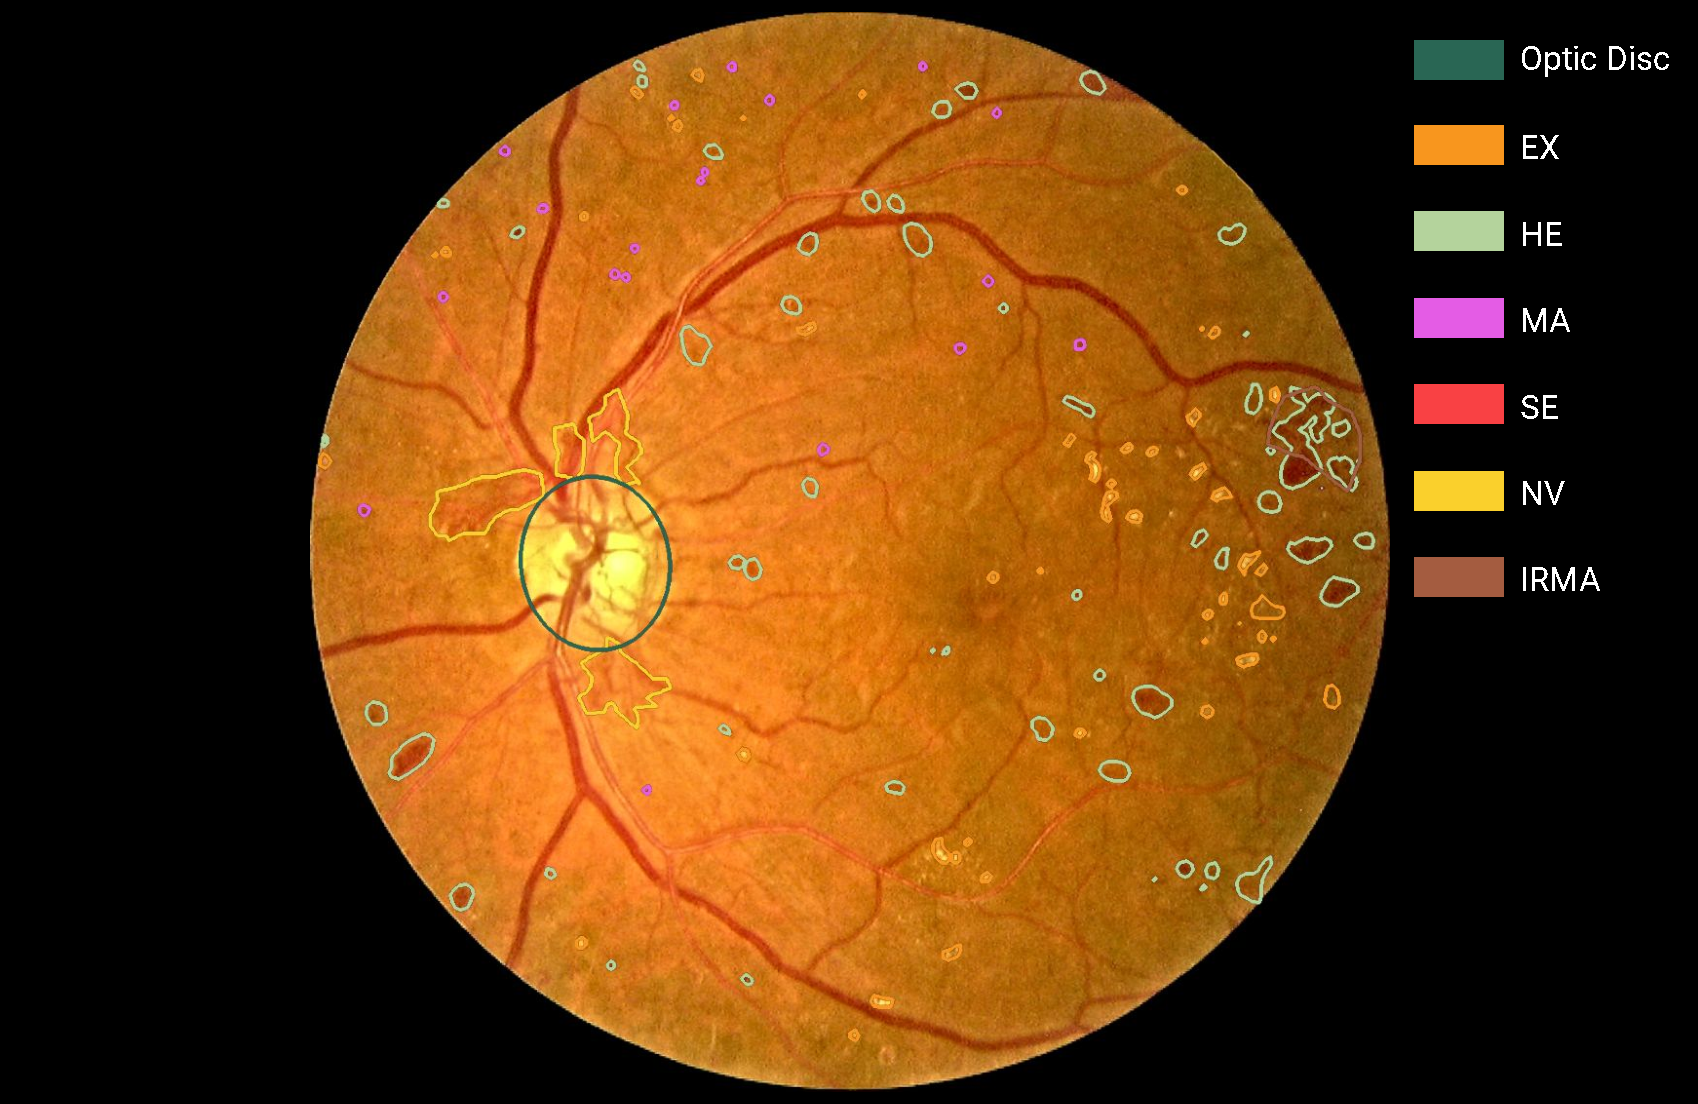
\includegraphics[width=\linewidth]{background/figs/retina.pdf}
    \caption{A retinal fundus image annotated with the optic disc as well as six types of lesions: hard exudates (EX), haemorrhages (HE), microaneurysms (MA), soft exudates (SE), neovascularization (NV), and intraretinal microvascular abnormalities (IRMA).}
    \label{fig:lesions}
\end{figure}
At the intersection of machine learning and DR detection there are a number of distinct, but related, research areas:
\begin{description}
    \item[Image-Level Grading] \hfill \\ To identify a DR severity grade for a fundus photograph. This can be according to the the international disease scale (summarised in \Cref{tab:dr_stages}), or a more coarse scale which combines several stages e.g. healthy, referred, diseased. For example, see \cite{Gulshan2016}. This task is difficult due to inter- and intra-grader variation, which causes datasets to be noisy.
    \item[Pixel-Level Segmentation] \hfill \\ To perform semantic segmentation of the retinal structure (blood vessels, optic disc) and/or lesions. For example, see \cite{Xiao_2019}.
    \item[Computer-Assisted Diagnosis] \hfill \\ To generate attention maps for suspicious areas, to be reviewed by a ophthalmologist. For example, see \cite{Wang2017}.
    \item[Image Synthesis] \hfill \\ To generate synthetic retinal fundus photographs. These could be conditioned on, for example, vascular structure or DR grade. This task is the subject of this project, and related work is discussed in greater detail in later sections.
\end{description}
\begin{table}[h]
    \centering
    \begin{tabular}{ll}
        \toprule
        Severity & Characteristics \\
        \midrule
        No apparent retinopathy & No abnormalities \\
        Mild NPDR & Microaneurysms only \\
        Moderate NPDR & More than just microaneurysms but less than severe NPDR \\
        Severe NPDR & Any of the following and no signs of PDR: \\ 
        & \tabitem > 20 intraretinal haemorrhages in all 4 quadrants \\
        & \tabitem Venous beading in $\geq$ 2 quadrants\\
        & \tabitem Intraretinal microvascular abnormalities in $\geq$ 1 quadrant \\
        PDR & One or both of: \\
        & \tabitem Neovascularisation \\
        & \tabitem Vitreous/preretinal haemorrhage \\
        \bottomrule
    \end{tabular}
    \caption{The International Clinical Diabetic Retinopathy Disease Scale \cite{ophthalmoscopy2002international}. \\ NPDR = non-proliferative diabetic retinopathy; PDR = proliferative diabetic retinopathy.}
    \label{tab:dr_stages}
\end{table}

\section{Generative Adversarial Networks} \label{sec:gans}

A Generative Adversarial Network (GAN) is a machine learning framework introduced by \citeauthor{gan} in \citeyear{gan} \cite{gan} consisting of two neural networks in adversarial competition. The generative model $G$ creates candidate images that look as ``real'' as possible, while the discriminative model $D$ attempts to distinguish between real and synthetic images. Training continues until the discriminator can no longer tell which inputs are fabricated by $G$ and which are real. In this sense, $G$ and $D$ are trained \emph{adversarially}. From this, we can derive the adversarial loss function by taking the cross-entropy of the real and generated samples:
\begin{align} \label{eq:ganloss}
    \mathcal{L}_{GAN} = \mathbb{E}_x[\log D(x)] + \mathbb{E}_z[\log (1-D(G(z))]
\end{align}
This yields the corresponding objective function:
\begin{align}
    \min_G \max_D \mathcal{L}_{GAN}
\end{align}
where $D(x)$ is the discriminator's estimate that $x \sim p_{data}$ is real; $G(z)$ is the generator's output when given random noise $z\sim p_z$; and $D(G(z))$ is the discriminator's estimate that a fake instance is real.
The discriminator will attempt to maximise this loss, whilst the generator attempts to minimise it.
In practice, this happens in alternating phases, keeping the generator fixed when updating the discriminator, and vice versa.
This means that the discriminator and generator can have differing loss functions instead of strictly adhering to the joint definition in \Cref{eq:ganloss}.

The versatility of GANs has enabled them to be applied to a plethora of problems including semantic segmentation and text generation, but their first and primary use is image synthesis.
The vanilla GAN design is far from perfect, however, and as such there has been an explosion of GAN variants since their initial introduction, making incremental improvements over each other.
In the following sections, we examine a selection of extensions and variants that are relevant to this project. 

Note that, while I have attempted to disentangle developments in GAN research over time by introducing these concepts in a coherent order, research does not always progress in a straight line, and new techniques do not always incorporate all the ideas of previous techniques.
Refer to \Cref{fig:conceptmap} for a holistic overview of how the discussed concepts relate to each other.

\begin{figure}
    \centering
    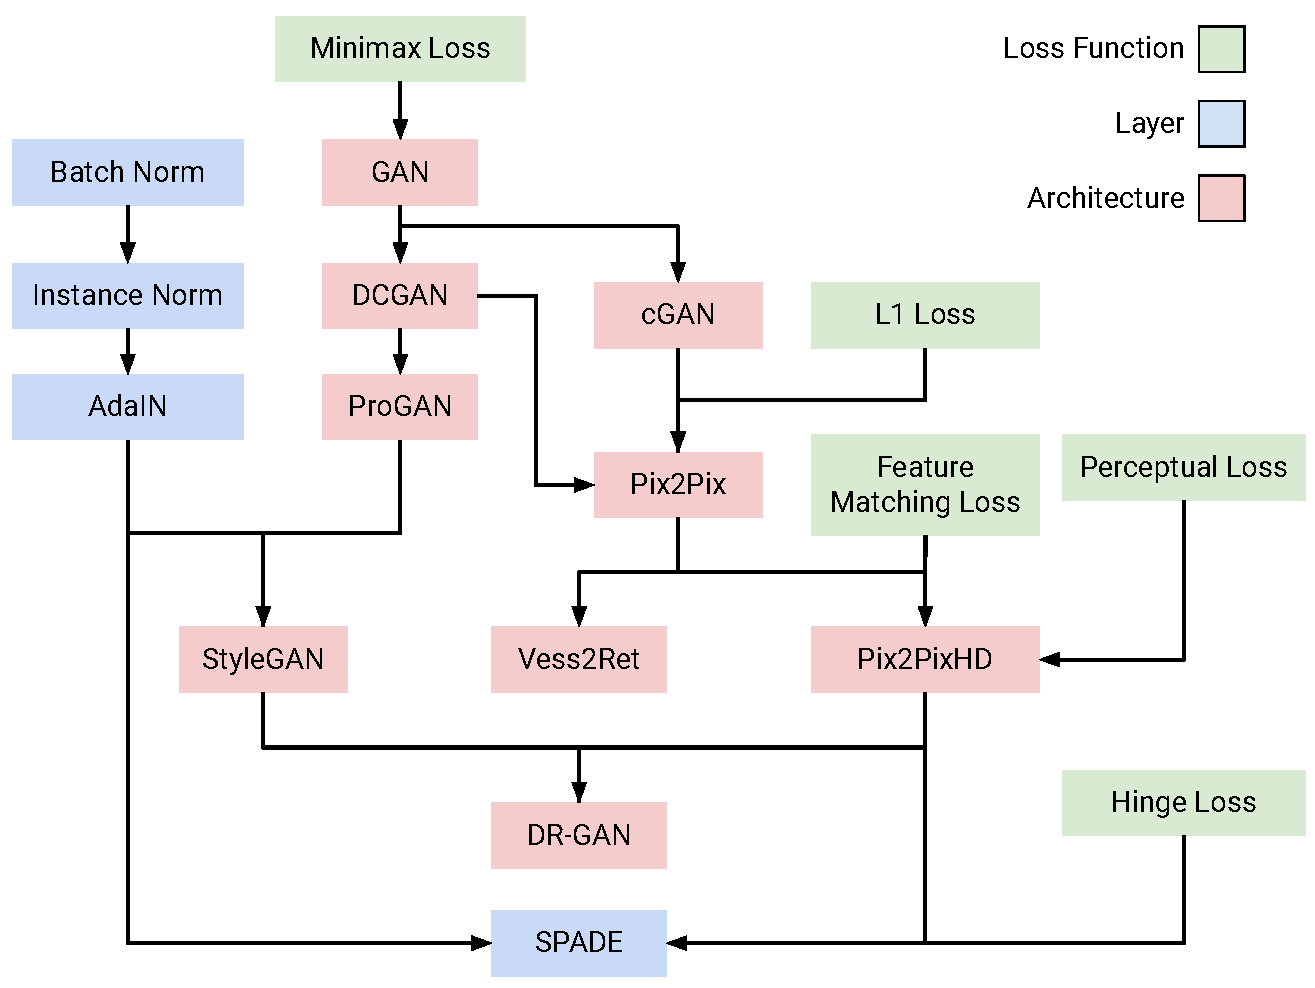
\includegraphics[width=0.6\textwidth]{background/figs/concept-map.pdf}
    \caption{Concept map of discussed techniques and how they relate to one another.}
    \label{fig:conceptmap}
\end{figure}

\section{Improving GAN Training}

Training GANs is known to be unstable, difficult to make converge, and prone to issues like mode collapse.
There have been a number of attempts to address these problems. 

\subsection{Modified Minimax Loss}

In their original paper, \citeauthor{gan} describe an issue with the original loss formulation where $G$ fails to gain any traction in the early stages of training, and therefore never even begins to converge.
This is due to $D$ being able to easily reject to the output of $G$, which causes the gradients to be extremely small.
To mitigate this, the authors propose to maximise $\log D(G(z))$ instead of minimising $\log(1-D(G(z))$ as in \Cref{eq:ganloss} i.e. the generator loss (denoted by superscript $G$) becomes
\begin{align}
    \mathcal{L}_{MM}^G = - D(G(z))
\end{align}
However, even this loss function is prone to vanishing gradients, and as a result other types of adversarial losses such as Wasserstein and Hinge loss have also been proposed.
These alternatives aim to provide consistently strong gradients throughout training.

\subsection{Feature Matching Loss} \label{sec:featurematching}

Even with the above modification, GANs can still fail to converge (i.e. the generator and discriminator fail to reach a Nash equilibrium).
This is because when the one network gets closer to the equilibrium, it can cause the other to move further from the equilibrium.
This oscillation can increase over time, causing divergence.
To address this, in \citeyear{salimans2016} \citeauthor{salimans2016} proposed a modification to the loss function called the feature matching loss \cite{salimans2016}.
In this scheme, instead of asking the generator to directly match the output of the discriminator, we ask it only to match some statistic of the real data.
These statistics are retrieved from an intermediate layer, $i$, of the discriminator, denoted by $D^{(i)}$:
\begin{align} \label{eq:fmloss}
    \mathcal{L}_{FM}^G = \left\lVert \mathbb{E}_x [ D^{(i)}(x)] - \mathbb{E}_z [D^{(i)}(G(z))] \right\rVert
\end{align}
where $\lVert \cdot \rVert$ is some norm, usually $L_1$ or $L_2$.

\subsection{Perceptual Loss}

Perceptual loss\footnote{This has also been called the ``content representation loss'' \cite{Gatys2016} and ``feature reconstruction loss \cite{johnson2016} in the literature.}, closely related to feature matching loss\footnote{The distinction between feature matching and perceptual losses is not entirely clear, with some publications even using terms interchangeably \cite{chen2017}. Here, we will use ``feature matching loss'' to refer to \Cref{eq:fmloss} and ``perceptual loss'' to refer to \Cref{eq:perceptualloss}.}, refers to the idea of defining a loss function in terms of a separate network $F$ in which image features are encoded \cite{Dosovitskiy2016}.
We take the loss as the distance between the two feature representations.
\begin{align} \label{eq:perceptualloss}
    \mathcal{L}_{P}^G = \left\lVert  F^{(i)}(x) - F^{(i)}(G(z)) \right\rVert
\end{align}
It has been shown that, in convolutional neural networks, perceptual losses measure the similarity of images in a more robust manner compared to per-pixel losses \cite{johnson2016}. 
A popular choice for network $F$, called the perceptual network, is VGG.

\subsection{Batch Normalisation} \label{sec:batchnorm}

During training, the distribution of the inputs into any given layer will constantly be changing as the parameters of preceding layers change -- a phenomenon known as ``internal covariate shift''.
This means that the current layer must keep readjusting to ever-changing distributions.
With deeper neural networks, this effect is amplified as changes in scale propagate down the layers.
Therefore, in order to keep training stable it is necessary to use lower learning rates, causing training to be slow overall.
To address this, \citeauthor{batchnorm} proposed a method called batch normalisation\footnote{While batch normalisation has been shown to be empirically effective, it has since been argued that the ``internal covariate shift'' explanation does not hold water \cite{lipton2018troubling, santurkar2019does}.}.
When applied to a particular layer, the input of said layer is re-centred (to zero mean) and re-scaled (to unit standard deviation) across the batch and spatial dimensions for each channel \cite{batchnorm}.
This allows for the use of larger learning rates since we do not run the risk of exploding gradients, which in turn enables faster training overall.

This normalising step means that the layer's activations will be unaffected by changes in scale in previous layers.
However, the authors point out that by normalising a layer we may change what the layer is capable of representing. 
To restore the ``representational power'' of the layer, we now \emph{denormalise} the normalised activations by performing an affine transformation using learned parameters. Note how this transformation is still independent of the distribution of activations in previous layers.

Formally, consider a batch of feature maps $X \in \mathbb{R}^{N\times C\times H\times W}$.
We can compute the mean and standard deviation for each channel $c$ as
\begin{align}
    \mu_c(X) &= \frac{1}{NHW} \sum_{n=1}^N \sum_{h=1}^H \sum_{w=1}^W X_{nchw} \label{eq:bnmean} \\ 
    \sigma_c(X) &= \sqrt{\frac{1}{NHW} \sum_{n=1}^N \sum_{h=1}^H \sum_{w=1}^W \left(X_{nchw}-\mu_c(X)\right)^2} \label{eq:bnstd}
\end{align}
Then the batch transform for each element is given by
\begin{align}
    \text{BN}_{\gamma, \beta}(X_{nchw}) = \gamma_c \left( \frac{X_{nchw}- \mu_c(X)}{\sigma_c(X)}\right) + \beta_c
\end{align}
where $\gamma, \beta \in \mathbb{R}^C$ are the per-channel transformation parameters.

\section{Image Synthesis}

This section establishes variations on GANs that establish the current state-of-the-art in image synthesis.

\subsection{Hierarchical GANs} \label{sec:hierarchgan}

The original paper detailing GANs by \citeauthor{gan} uses the MNIST dataset as a demonstration of the capability of GANs.
These images are very low-resolution, at just $28\times 28$ pixels, due to the fact that the original approach did not scale well to high-resolution images.

In classical computer vision, the concept of a Laplacian pyramid on which filters can operate on multiple different scales is well established \cite{1095851}. Extending this idea to GANs, one of the first attempts at improving high-resolution image synthesis was LAPGAN, introduced by \citeauthor{DBLP:journals/corr/DentonCSF15} in 2015 \cite{DBLP:journals/corr/DentonCSF15}, where a separate generative CNN is trained at each scale. 
Since then, variants on this key insight of ``stacking'' models that operate on different scales has been explored thoroughly, whether it is stacking entire GANs \cite{DBLP:journals/corr/HuangLPHB16}, stacking only discriminators \cite{TCWang2017}, or stacking only generators \cite{DBLP:journals/corr/GhoshKNTD17}. 

In spite of these advances, high-resolution image synthesis has remained difficult due to the fundamental fact that the increased detail makes it easier for the discriminator to distinguish real from generated images, amplifying the vanishing gradient problem that has historically plagued GAN training. 

\subsection{DCGAN}

The difficulty of scaling up a GAN with CNNs to generate high-resolution images led to LAPGAN's alternative approach of leveraging multiple separate CNNs.
Deep Convolutional GANs (DCGAN) are a class of GAN architectures proposed by \citeauthor{dcgan} in \citeyear{dcgan} \cite{dcgan}.
In their paper, the authors outline a set of constraints that should be adhered to in order to create GANs which can produce higher-resolution images, and whose training is more stable.
\begin{itemize}
    \item Use strided convolutions in the discriminator and fractional-strided convolutions in the generator instead of pooling layers.
    \item Use batch normalisation in the generator and discriminator.
    \item Remove fully-connected layers.
    \item Use ReLU activation for all layers in the generator, except the output which should use $\tanh$.
    \item Use leaky ReLU activation for all layers in the discriminator.
\end{itemize}

\subsection{Progressive Growing GAN}

Building on these ideas, progressive growing GANs (ProGAN) were introduced by \citeauthor{DBLP:journals/corr/abs-1710-10196} in \citeyear{DBLP:journals/corr/abs-1710-10196} \cite{DBLP:journals/corr/abs-1710-10196}.
The fundamental idea is that instead of training all layers at once, we incrementally \emph{grow} both the discriminator and generator during training, starting from low-resolution images up to high-resolution images.
With each additional layer that is faded in, finer details at higher resolutions are able to be added.
This allows for the stable training of generator models that are capable of producing high-quality images.

\subsection{Instance Normalisation} 

Instance normalisation is similar in concept to batch normalisation, but we just normalise the inputs across the only the spatial dimensions for each sample \emph{and} channel.
Although batch normalisation was introduced with the intention of improving the rate of training, in \citeyear{instancenorm} \citeauthor{instancenorm} found that just by replacing batch normalisation with instance normalisation, the \emph{visual quality} of certain image synthesis networks could be significantly improved \cite{instancenorm}.

Consider, as in \Cref{sec:batchnorm}, a batch of feature maps $X\in \mathbb{R}^{N \times C \times H \times W}$.
We can compute the mean $\mu_{nc}$ and standard deviation $\sigma_{nc}$ for each sample and channel as
\begin{align}
    \mu_{nc}(X) &= \frac{1}{HW} \sum_{h=1}^{H} \sum_{w=1}^W X_{nchw} \\
    \sigma_{nc} &= \sqrt{\frac{1}{HW} \sum_{h=1}^H \sum_{w=1}^W \left(X_{nchw}-\mu_{nc}(X)\right)^2}
\end{align}
Note the differences between this and the definitions used in batch normalisation (\Cref{eq:bnmean} and \eqref{eq:bnstd}). Then the instance normalisation transform for each element is given by
\begin{align}
    \text{IN}_{\gamma, \beta}(X) = \gamma_c \left( \frac{X_{nchw} - \mu_{nc}(X)}{\sigma_{nc}(X)} \right) + \beta_c
\end{align}
where $\gamma, \beta \in \mathbb{R}^C$ are the per-channel transformation parameters.

\subsection{AdaIN} \label{sec:adain}

Adaptive Instance Normalisation (AdaIN) is a conditional extension to instance normalisation introduced in \citeyear{adain} by \citeauthor{adain} \cite{adain}, meaning that it uses external information to learn the denormalisation parameters $\gamma, \beta$.
In contrast, standard instance normalisation and batch normalisation are unconditional normalisation layers.
AdaIN takes a content input $X$ and an adaptive style input $Y$, and aligns the mean and variance of $X$ with those of $Y$.
Unlike batch normalisation or instance normalisation, its parameters are not learned but instead adaptively computed from $Y$.
\begin{align}
    \text{AdaIN} (X, Y) = \sigma_{nc}(Y) \left( \frac{X_{nchw} - \mu_{nc}(X)}{\sigma_{nc}(X)} \right) + \mu_{nc}(Y)
\end{align}
Intuitively, we can understand this operation as applying the style of $Y$ to $X$. Despite being first developed for style transfer, AdaIN was later adapted for a variety of other computer vision tasks.

\subsection{StyleGAN} \label{sec:stylegan}

\begin{figure}[h]
    \centering
    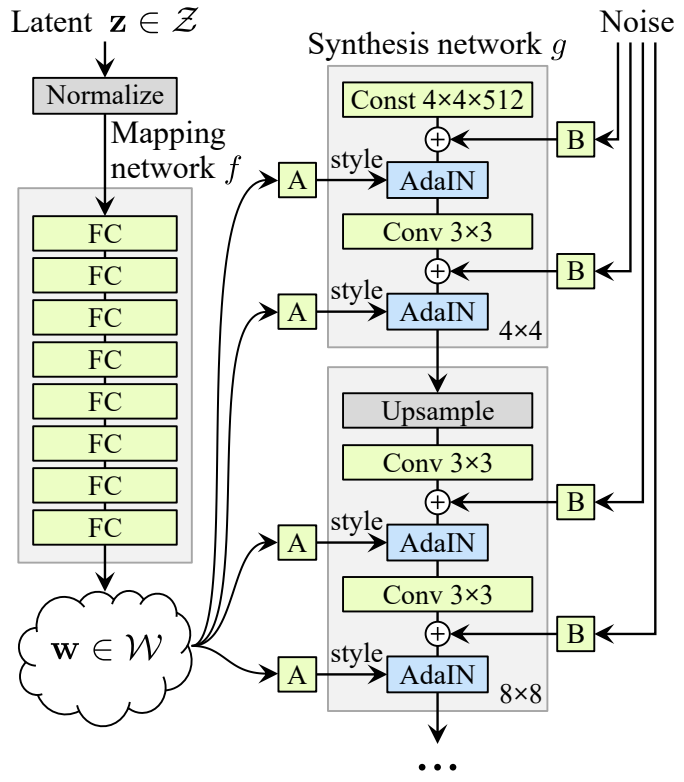
\includegraphics[width=0.5\textwidth]{background/figs/stylegan.png}
    \caption{Diagram of the StyleGAN generator architecture. Taken from \cite{stylegan}.}
    \label{fig:styleganarch}
\end{figure}

Introduced in \citeyear{stylegan} by \citeauthor{stylegan}, StyleGAN combines both AdaIN and progressive growing to produce high-resolution photo-realistic images.
Up until now, we have been providing a linear, feed-forward neural network generator a latent code $z \in \mathcal{Z}$ at the input layer.
Instead, StyleGAN introduces a generator architecture in which a vector in the intermediate latent space $w \in \mathcal{W}$ is supplied to AdaIN layers after each convolutional layer.
\Cref{fig:styleganarch} shows this new architecture and the role of the mapping network.
The intermediate latent space $\mathcal{W}$ is learned by a mapping network, and the point in the network at which provide $w$ is provided is correlated with how coarse or fine the transferred features are.

\section{Conditional Image Generation}

Having discussed the progression of \emph{unconditional} high-resolution image generation, we now turn to work done in the field of \emph{conditional} image generation. 
We start by looking at how GANs can be guided to generate images of a certain class, and then at the specific task of image-to-image synthesis, wherein an input image (such as a semantic label map) is transformed to an output image (such as a retinal fundus image). 

\subsection{Conditional GAN}

One of the earliest extensions to the original design, a conditional GAN (cGAN) extends the vanilla GAN by conditioning on additional information $y$, allowing us to direct the generation process \cite{DBLP:journals/corr/MirzaO14}.
Consequently, the loss function previously defined in \Cref{eq:ganloss} now becomes
\begin{align} \label{eq:cganloss}
    \mathcal{L}_{cGAN} = \mathbb{E}_{x, y}[\log D(x|y)] + \mathbb{E}_{y, z}[\log (1-D(G(z|y))]
\end{align}
Today, there are four well-understood methods of conditioning the generator:
\begin{itemize}
    \item concatenation of a vector representing the label;
    \item adding an auxiliary classifier;
    \item using projection; and
    \item conditional batch normalisation.
\end{itemize}

\subsection{Pix2Pix} \label{sec:pix2pix}

In \citeyear{pix2pix}, \citeauthor{pix2pix} introduced pix2pix, a conditional GAN for general purpose image-to-image translation (as opposed to class-conditional image generation), capable of producing photo-realistic images from a semantic label map \cite{pix2pix}.
First, inspired by \cite{DBLP:journals/corr/PathakKDDE16}, the authors added a global reconstruction loss penalty to the basic adversarial cGAN objective (\Cref{eq:cganloss}), implemented using the $L_1$ norm.
\begin{align}
    \mathcal{L}_{L_1} = \mathbb{E}_{x, y, z} \left\lVert x - G(z|y) \right\rVert_1
\end{align}
This captures the overall structure of the image, and therefore serves to prevent the generator from creating synthetic images that deviate too far from the real image. 
Together, this yields the overall objective function
\begin{align} \label{eq:pix2pixloss}
    \mathcal{L}_{pix2pix} = \mathcal{L}_{cGAN}(G, D) + \lambda \mathcal{L}_{L_1}(G)
\end{align}
where $\lambda$ is a hyperparameter that balances the contribution of the two terms.

Next, they iterate on the DCGAN generator and discriminator architectures. For the generator, skip-connections are added to the standard encoder-decoder architecture, resembling that of a U-Net \cite{unet}, used to directly share information across the network.
Turning to the discriminator, the authors identified that since the $L_1$ loss from above already enforces correctness at the larger scale, the discriminator need only penalise at smaller scales.
For this reason, they opted for a patch-based CNN discriminator which calculates loss for $N\times N$ patches, where $N$ is smaller than the image size.

\subsection{Pix2PixHD}

While promising, pix2pix was only designed to generate images at resolutions up to $512\times 512$.
Attempting to apply pix2pix to higher resolution images resulted in unstable training, and blurry details in the generated images.
To address these issues, in \citeyear{pix2pixhd} \citeauthor{pix2pixhd} released pix2pixHD \cite{pix2pixhd} as an extension to pix2pix. 

Building on the idea of a hierarchical GAN structure, a multi-scale generator is adopted to work on images of different resolutions.
In their paper, the authors choose to use two sub-networks with one acting as a ``global generator'' and the other a ``local enhancer''.

Similarly, multi-scale discriminators operating at three different scales are employed.
This works slightly differently to the multi-scale generators, since instead of having a nested sub-network, three separate networks are used.

The adversarial loss defined in \Cref{eq:pix2pixloss} is improved by adding a feature matching loss.
Together, we get the overall objective:
\begin{align} \label{eq:pix2pixhdloss}
    \min_G \Bigg( \bigg( \max_{D_1, D_2, D_3} \sum_{k=1, 2, 3} \mathcal{L}_{GAN} (G, D_k) \bigg) + \lambda_{FM} \sum_{k=1, 2, 3} \mathcal{L}_{FM} (G, D_k) \Bigg)
\end{align}
The discriminator's objective is maximised over each of the discriminators, and that $D_k$ does not maximimise $\mathcal{L}_{FM}$, serving only as a feature extractor. 
They also found that adding perceptual loss using a pre-trained VGG network slightly improved results, but was not critical.
With the perceptual loss, we have the objective:
\begin{equation} \label{eq:pix2pixhdloss2}
\begin{split}
    \min_G & \Bigg(\bigg( \max_{D_1, D_2, D_3} \sum_{k=1, 2, 3} \mathcal{L}_{GAN} (G, D_k) \bigg) \\
           &\quad + \lambda_{FM} \sum_{k=1, 2, 3} \mathcal{L}_{FM} (G, D_k) \\
           &\quad + \lambda_{P} \min_{D_k} \sum_{k=1, 2, 3} \mathcal{L}_{P} (G, D_k) \Bigg)
\end{split}
\end{equation}
To enhance object edges, instance boundary maps are used.

\section{Metrics}

We introduce some more uncommon metrics that the may be unfamiliar to the reader.

\subsection{Fréchet Inception Distance}

The Fréchet Inception Distance (FID) \cite{fid} is a metric for assessing the ``quality'' and diversity of generated images by comparing the distribution of the images used to train the generator with the distribution of generated images.
Specifically, feature vectors from a pre-trained Inception-v3 network \cite{inceptionv3} are used to build the distribution $\mathcal{N}(\mu, \Sigma)$ on the generated images, and the distribution $\mathcal{N}(\mu_w, \Sigma_w)$ on real images. 
Then, we calculate the FID score as the Wasserstein metric between these two distributions:
\begin{align}
    \text{FID} = \lvert \mu - \mu_w \rvert^2 + \text{tr}(\Sigma + \Sigma_w - 2(\Sigma \Sigma_w))^\frac{1}{2}
\end{align}
In essence, a smaller FID indicates a smaller distance between the two distributions.
FID is not without its issues \cite{improved_precision}, however it remains the most popular GAN evaluation metric as of today.

In this work, we use Maximilian Seitzer's PyTorch implementation of the FID score\footnote{\url{https://github.com/mseitzer/pytorch-fid}}, with feature vectors extracted from the final average pooling layer of the Inception network.

\subsection{Cohen's Quadratic Weighted Kappa}

Cohen's kappa, $\kappa$, is a metric which measures the degree of agreement between two raters who each classify $N$ items into $C$ mutually exclusive categories.
$\kappa = 1$ indicates complete agreement, $\kappa = 0$ indicates random agreement, and $\kappa < 0$ indicates worse than random agreement.
It is calculated by
\begin{align}
    \kappa = \frac{p_o - p_e}{1 - p_e}
\end{align}
where $p_o$ is the observed probability of agreement, and $p_e$ is the probability of random agreement.
We can also generalise this statistic to the weighted kappa, which is useful when some disagreements are more important than others.
In our case, we use quadratic weighting, calculated as
\begin{align}
    \kappa = 1 - \frac{\sum_{i=1}^k \sum_{j=1}^k w_{ij}x_{ij}}{\sum_{i=1}^k \sum_{j=1}^k w_{ij} m_{ij}}
\end{align}
Cohen's quadratic weighted kappa is used as the primary metric by both Kaggle DR grading competitions.

\chapter{Related Work} \label{cha:relatedwork}

We now set the research context in which to understand this project's contributions.

\section{Retinal Image Synthesis} \label{sec:retinalimagesynthesis}

% Automatic Generation of Synthetic Retinal Fundus Images (Fiorini 2014)
% Towards Adversarial Retinal Image Synthesis (Costa 2017)
% Adversarial Synthesis of Retinal Images from Vessel Trees
% End-to-End Adversarial Retinal Image Synthesis (Costa 2017)
% Unsupervised histopathology image synthesis (2017)
% Synthesizing retinal and neuronal images with generative adversarial nets (Tub-GAN) (2018)
% Retinal image synthesis from multiple-landmarks input with generative adversarial networks (2019)
% DR GAN (2020)

Early work surrounding the generation of synthetic retinal fundus images involved patch-based techniques and complex mathematical models representing the anatomy of the eye \cite{BONALDI201654, N20103:2014}.
Different algorithms had to be proposed for different components of the eye, relying heavily on domain knowledge.

\subsection{Vess2Ret}

More recently, purely data-driven approaches have been shown to be highly effective.
In \citeyear{Costa2017}, \citeauthor{Costa2017} published their foundational work utilising GANs for retinal image synthesis, dubbed vess2ret \cite{Costa2017}.
The proposed generator network operated by performing image-to-image translation from a vessel network to a retinal fundus image.
Like pix2pix, they add a global $L_1$ loss term, using \Cref{eq:pix2pixloss} as their loss function.
In the absence of a large dataset containing manual annotations, vessel masks were inferred from the output of a segmentation model.
The network architectures also resemble those of pix2pix, using a U-Net architecture for the generator and patch-based CNN for the discriminator.

However, this approach still suffers some major drawbacks. 
The fact that the generator relies on a vessel segmentation mask as input is unideal since the user will have to either (a) manually obtain their own vessel segmentation; (b) use a pre-existing vessel segmentation, of which there is a limited pool; or (c) infer a vessel segmentation (as the authors did) which may be unreliable.
Moreover, since a vessel segmentation maps to exactly one synthetic retina, data diversity is naturally limited.
The authors note that a poorly inferred vessel network, as may be produced by a segmentation model, fails to produce a usable fundus image. 
The output images have a resolution of $512 \times 512$ which, while large relative to the images often used in computer vision publications at the time, is small compared to those produced by modern fundus photography.
% \begin{figure}
%     \centering
%     \begin{subfigure}{0.3\textwidth}
%         \centering
%         \includegraphics[width=\textwidth]{example-image-a}
%         \caption{Generator architecture used in vess2ret \cite{Costa2017}.}
%         \label{fig:costa2017gen}
%     \end{subfigure}
%     \hspace{0.1\textwidth}
%     \begin{subfigure}{0.3\textwidth}
%         \centering
%         \includegraphics[width=\textwidth]{example-image-b}
%         \caption{Discriminator architecture used in vess2ret \cite{Costa2017}.}
%         \label{fig:costa2017dis}
%     \end{subfigure}
% \end{figure}

The same authors extend this existing architecture in a later work by removing the dependency on a pre-existing vessel segmentation as input \cite{Costa2018}.
Instead, an adversarial autoencoder is employed to generate vessel segmentation masks, which can be fed into the previously described image-to-image model.
This requires the user to simply supply a sample from a multivariate normal distribution, which means that a theoretically unbounded number of different vessel segmentations can be generated (although this does not speak for diversity).
While this overcomes the first of the issues with the previous work by obviating the need for the user to obtain a segmentation mask, the generated vasculatures are prone to displaying abnormalities, and the issue of resolution remains.

\subsection{Tub-GAN}

\citeauthor{tubgan} \cite{tubgan} incrementally built upon this work in \citeyear{tubgan} by introducing Tub-GAN. 
It resembles its predecessor in that the same loss function is used, and the generator architecture is also based on U-Net, except using $\tanh$ in the output layer instead of the sigmoid function.
They depart from vess2ret, however, in their discriminator design. Instead of using a patch-based CNN, a DCGAN is used, consisting of Convolution-BatchNorm-LeakyReLU blocks.
The notable improvements are the fact that manual annotations are used for training, and that the generator takes a noise code which allows for stochastic variation in the outputs from a single vessel segmentation.
However, in the absence of a vessel generator, it reinstates a dependency on a pre-existing vessel network annotation.
% \begin{figure}
%     \centering
%     \begin{subfigure}{0.3\textwidth}
%         \centering
%         \includegraphics[width=\textwidth]{example-image-a}
%         \caption{Generator architecture used in TubGAN \cite{tubgan}.}
%         \label{fig:zhao2018gen}
%     \end{subfigure}
%     \hspace{0.1\textwidth}
%     \begin{subfigure}{0.3\textwidth}
%         \centering
%         \includegraphics[width=\textwidth]{example-image-b}
%         \caption{Discriminator architecture used in TubGAN \cite{tubgan}.}
%         \label{fig:zhao2018dis}
%     \end{subfigure}
% \end{figure}

While representing an important step towards the generation of synthetic fundus images, both Tub-GAN and vess2ret lack the ability to control the generation of pathological instances.
However, in the same publication, the authors also present a variant of Tub-GAN incorporating style transfer called Tub-sGAN which presents a possible solution to this limitation.
In the Tub-sGAN framework, a target style is provided alongside the input segmentation.
The output image is expected to posses the style of the target image, while retaining the structure dictated by the segmentation.
This is much more useful since we now have the ability to transfer the texture of pathological examples onto the existing vasculature, which should include its lesions.

Nonetheless, a few shortcomings are noted.
First, the generated images still exhibit failure cases when they are not anatomically correct, particularly with respect to the optic disc and macula.
Furthermore, while the style-transfer appears to work well for global texture, it performs poorly in synthesising fine local details.
This is problematic since many retinal lesions are extremely small.
Although the authors report increased segmentation performance of vasculatures, we are interested in the more challenging task of lesion segmentation, whose ground-truths are not supplied by this network.

\subsection{Retinal Pathological Descriptor}

In 2019, \citeauthor{Niu_2019} \cite{Niu_2019} proposed an interesting ``symptom transfer'' network which allowed for lesion manipulation by exploiting the neuronal activations of an existing image-level DR grading network. 
This allows them to arbitrarily augment the position and quantity of lesions in generated images.

While interesting in concept, there is no ability to directly condition the generation on DR severity or lesion segmentations.
Therefore, we consider this work orthogonal to our objectives.

\subsection{DR-GAN}

More recently, in \citeyear{Zhou_2020}\footnote{The 2020 work is an extension of preliminary work published in 2019.
We consider the extended work only, since it supersedes the preliminary work.} \citeauthor{Zhou_2020} introduced DR-GAN \cite{Zhou_2020}: a network that ensembles many of the discussed techniques and applies them to retina generation.
DR-GAN draws heavily from recent developments in image-to-image translation by incorporating feature matching loss; multi-scale generators and discriminators; instance boundary maps; spatial and channel attention; and adaptive instance normalisation.
By leveraging these methods, DR-GAN overcomes many of the limitation of prior work, taking into account image-level grade information, pixel-wise lesion labels, and optic disc instance masks.

The authors acknowledge that, due to the extremely small size of lesions, synthesis of fundus images must be done at a high resolution to be useful.
To deal with this, they employ multi-scale generators and discriminators similar to those used in pix2pixHD. 
In order to preserve very fine features, they use a spatial and channel attention module (SCA) in the synthesis blocks inspired by \cite{sca1}, which in turn is inspired by \cite{sca2}.
Recalling the techniques used in StyleGAN, each of the synthesis blocks also contains an AdaIN layer which gives the ability to manipulate the grade of the generated images using what the authors call ``adaptive grading vectors''.
The latent grading space is first learnt using the ResNet-50 network.
From this, a set of normal distributions representing the grading space are computed.
During synthesis, the appropriate distribution is sampled from and injected into the AdaIN component of synthesis blocks.
In this way, the ``style'' of the sampled vector is transferred to the generated image. 
They extend the pix2pixHD loss function by adding a classification loss $\mathcal{L}_C$, specifically focal loss \cite{focal}, to combat class imbalance. They use VGG-19 as their perceptual network.
\begin{equation}
\begin{split}
    \min_G & \Bigg(\bigg( \max_{D_1, D_2, D_3} \sum_{k=1, 2, 3} \mathcal{L}_{GAN} (G, D_k) \bigg) \\
           &\quad + \lambda_{FM} \sum_{k=1, 2, 3} \mathcal{L}_{FM} (G, D_k) \\
           &\quad + \lambda_{P} \min_{D_k} \sum_{k=1, 2, 3} \mathcal{L}_{P} (G, D_k) \\
           &\quad + \lambda_{C} \min_{D_k} \sum_{k=1, 2, 3} \mathcal{L}_{C} (G, D_k) \Bigg)
\end{split}
\end{equation}
DR-GAN represents the state-of-the-art at the time of writing, incorporating some of the most recent techniques in computer vision.
The authors are able to demonstrate quantitatively the improvements in image quality over previous methods, and briefly show how synthetic data can improve classification performance. However, the effect of synthetic data on segmentation performance is not discussed. The model is still held back by limitations in the training data, and hence still exhibits a number of failure cases. DR-GAN still relies upon inferred structural and lesion segmentation masks to bootstrap its training due to the lack of manually annotated data. 

One concern that is unclear from the paper is how these adaptive grading vectors interact with the lesions of the input mask.
For instance, if a lesion mask exhibiting proliferative DR is given to the network, and during synthesis adaptive grading vectors corresponding to a healthy retina are provided, what will the resulting output resemble? 
And will the lesion mask still be useful if the lesions have been manipulated?
Without the source code, these questions remain unanswered.

\section{Semantic Label Generation}

Meanwhile, literature on the task of semantic label generation is relatively sparse.
\citeauthor{wang2016} \cite{wang2016} first introduced this factorisation into ``structure'' and ``texture'' in \citeyear{wang2016} when attempting to first generate normal maps which encode the geometry of the scene, and from this generating a realistic 2D image.
Their ``Structure-GAN'' generates small $72\times72\times3$ images, and the generator is deeper than the discriminator.
They also apply joint fine-tuning of both networks together, after training each one independently.

Later, in \citeyear{ghelfi2019}, \citeauthor{ghelfi2019} \cite{ghelfi2019} introduced a variant of the GAN where the last layer is simply replaced by a softmax layer.
The authors describe this as a ``more principled'' approach to generating semantic images, as opposed to treating them like standard RGB images, as in \citeauthor{wang2016}'s earlier work.
However, beyond that the papers insights into the challenges unique to this domain are limited.

More recently, in \citeyear{volokitin2020}, \citeauthor{volokitin2020} \cite{volokitin2020} went on to apply a similar technique to demonstrate how the generation of natural images could be separated into the distinct steps of layout prediction and texturing.
As opposed to improving segmentation performance, they were instead motivated by how this decomposition could improve the plausibility of multi-object scenes.
To generate semantic labels they used a DCGAN architecture, and a pix2pix model for image texturing.

Concurrently, \citeauthor{azadi2019} \cite{azadi2019} introduced a method in which the two components are trained independently at first, then fine-tuned by training in an end-to-end fashion, resembling the aforementioned Structure-GAN by \citeauthor{wang2016}.
This approach was dubbed the ``Semantic Bottleneck GAN'', or SB-GAN.
The authors note how the task of learning the interactions between structural elements to generate discrete labels is ``extremely challenging''.
However, the focus of their work was generating high-fidelity images, and did not study the effect on downstream tasks.
Moreover, the end-to-end fine-tuning was done by introducing an additional, unconditional discriminator, trained to distinguish real RGB images and those generated from synthetic layouts.
This is likely to weaken the conditioning between the semantic labels and the output image, potentially making this approach inappropriate for our use case since we would like to use the semantic labels as segmentation maps.

Moreover, none of these approaches attempt class-conditioning of semantic labels, nor do they evaluate the effect of synthetic data on downstream tasks.
A further complication is that the semantic labels of interest to us are far sparser than those used in the datasets of previous work.

\section{Training on Synthetic Data}

There already exists a history of synthetic data already being used to train machine learning models; however this work has largely been to do with using 3D scenes to train 2D computer vision algorithms (\cite{gaidon2018} provides a good overview).
Regardless, this has built a case that synthetic data could result in a real-world improvement. 
As early as \citeyear{gaidon2016}, \citeauthor{gaidon2016} \cite{gaidon2016} showed that pre-training on synthetic data and subsequent fine-tuning on real data could improve the performance of computer vision algorithms. 

Even closer to our mixed-data approach, \citeauthor{shrivastava2016} \cite{shrivastava2016} showed that training on a mixture of real and synthetic data improved performance of pose estimation models, compared to training on only real data.


\chapter{Data} \label{cha:data}

In this chapter, we survey the available datasets and examine how their characteristics may influence our models.
For our work to be of any practical use, it is imperative that we collect data that is as diverse as possible, representing a wide range of imaging conditions and patient backgrounds.
While large datasets for image-level graded images are available, the lesion segmentation task suffers from a severe lack of pixel-wise segmented data, and even fewer provide both grading and semantic label information.

In the field of data science, fully understanding the properties of your data domain is just as imperative as model development.
Exploratory data analysis provides the necessary context and insights to choose the appropriate modelling techniques and put forth an informed interpretation of one's results.

\section{FGADR}

\begin{figure}[h]
    \centering
    \begin{subfigure}{0.45\textwidth}
        \centering
        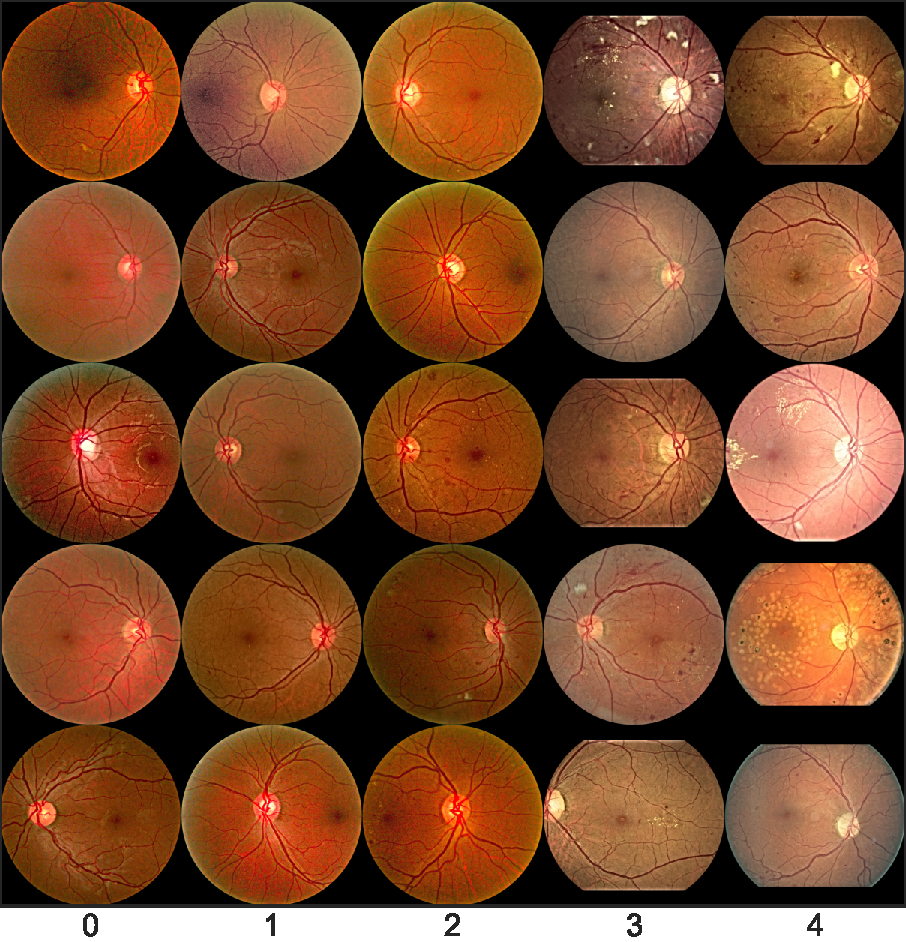
\includegraphics[width=\linewidth]{datasets/figs/fgadr_real_sample.pdf}
        \caption{Retinal fundus images.}
        \label{fig:fgadr_sample_real}
    \end{subfigure} %
    \begin{subfigure}{0.45\textwidth}
        \centering
        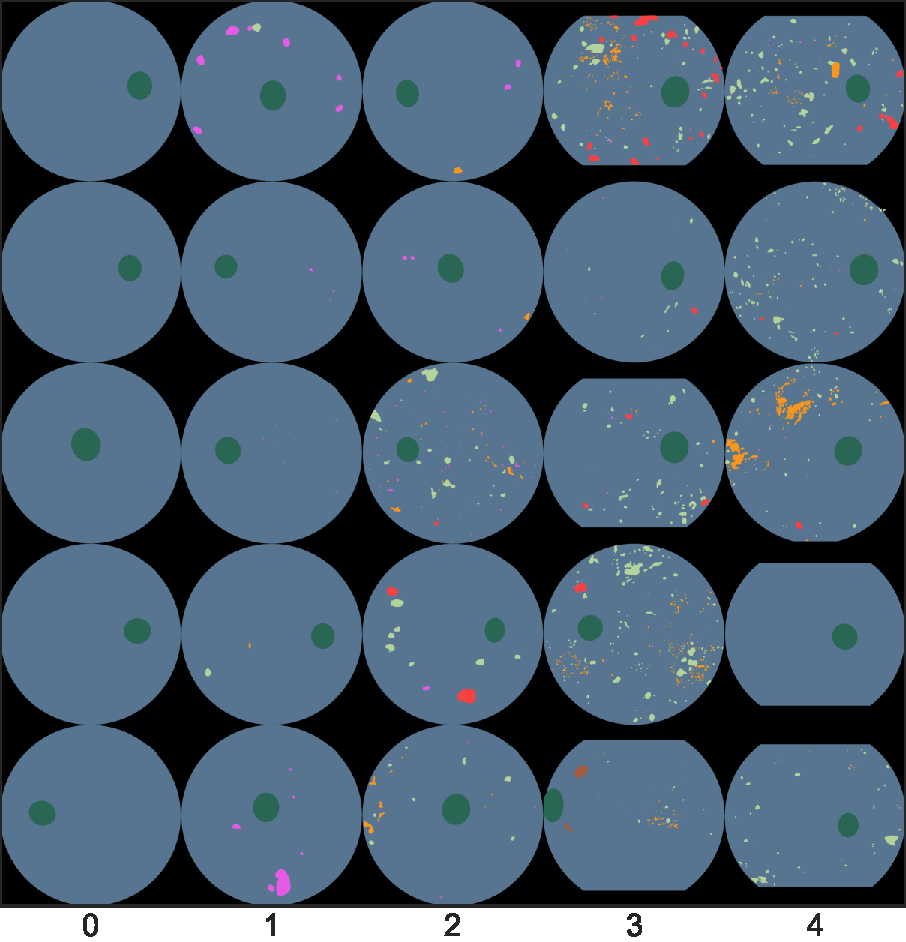
\includegraphics[width=\linewidth]{datasets/figs/fgadr_label_sample.pdf}
        \caption{Corresponding semantic labels.}
        \label{fig:fgadr_sample_label}
    \end{subfigure}
        \caption{A sample of images from the FGADR dataset and accompanying manual semantic annotations. Columns from left to right correspond to DR grades 0 through 4.}
    \label{fig:fgadr_sample}
\end{figure}

The Fine-Grained Annotated Diabetic Retinopathy (FGADR) dataset \cite{Zhou2020b} was released in 2020 alongside DR-GAN, and consists of two subsets.
The first, called the \emph{Seg-set}, contains 1842 images with both image-level annotations for DR severity, and pixel-level annotations for microaneurysms, haemorrhages, hard exudates, soft exudates, intraretinal microvascular abnormalities, and neovascularization.
Optic disc masks are not provided, so manual annotations were collected for this project (provided in \Cref{sec:od}).
The second, called the \emph{Grade-set}, contains 1000 images with only image-level DR grades.
It is useful for its high annotation confidence, however the \emph{Grade-set} is still pending approval by the researcher's legal department at the time of writing, and therefore is regrettably not available for use in this project.
All images in both sets have a resolution of $1280 \times 1280$.
This is the only pixel-wise annotated dataset that includes labels for neovascularization and intraretinal microvascular abnormalities, which is of particular significant since according to \Cref{tab:dr_stages}, NV and IRMA are key to differentiating stage 3 from stage 4.

\Cref{fig:fgadr_sample} shows a sample of images and associated annotations from the FGADR dataset.
Visually, the relationship between the prevalence of lesions and DR grade is clear.
Note that overlap of semantic labels is possible with the images.
We resolve these arbitrarily, based on the index of the label (according to \Cref{tab:mappings}).
The photographs themselves are noisier than those from the other datasets, which can likely be attributed to the illumination conditions at the time of imaging.

% \begin{figure}[h]
%     \centering
%         \centering
%         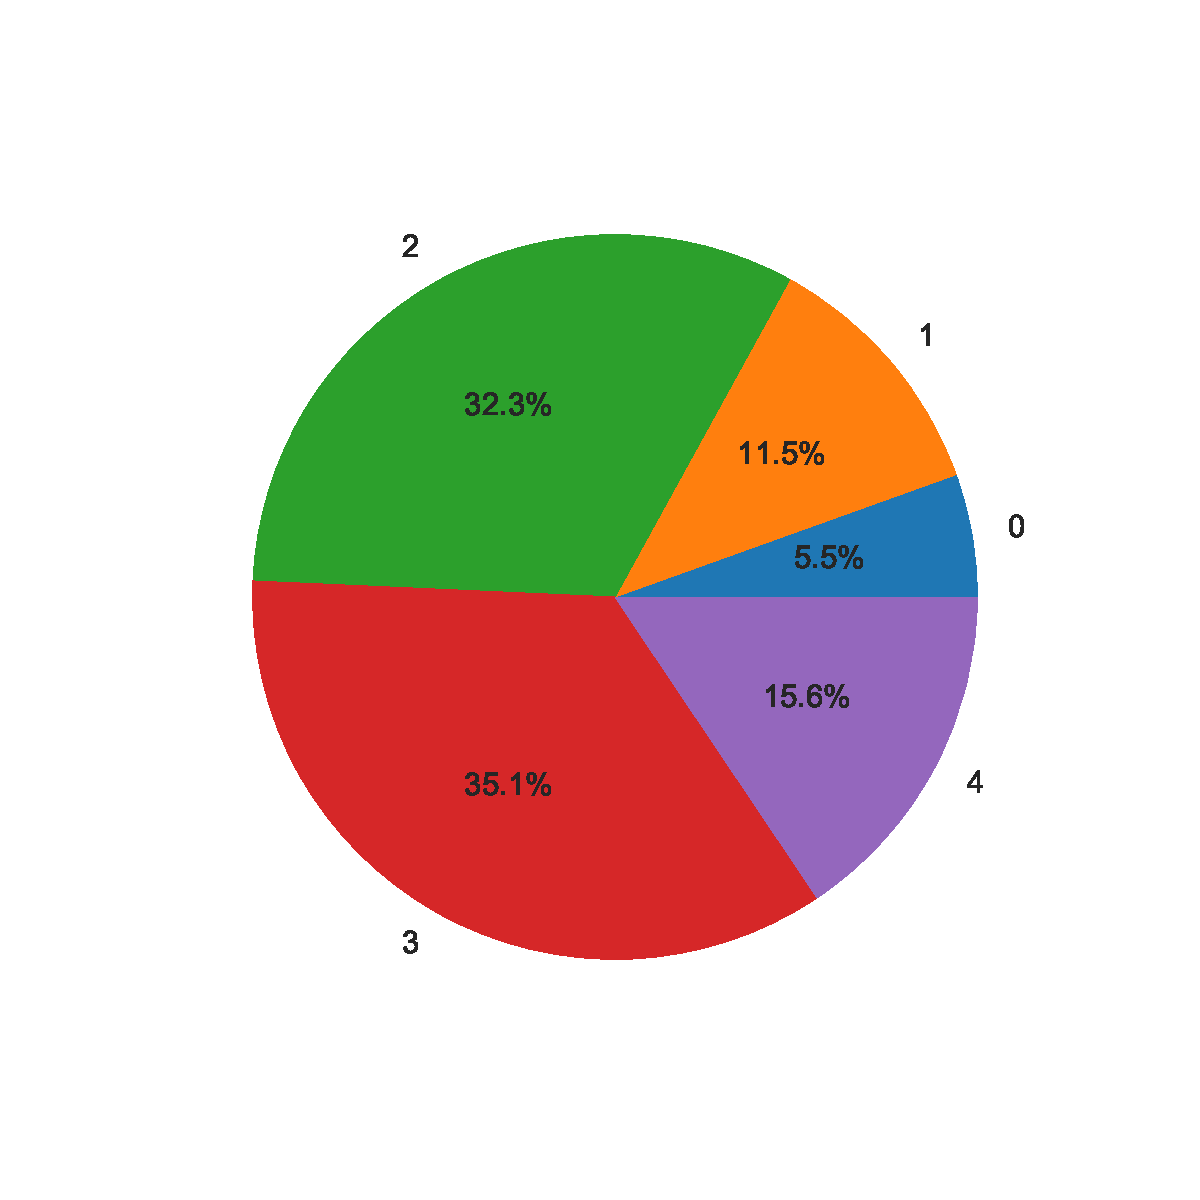
\includegraphics[width=0.5\textwidth]{datasets/figs/fgadr_grade_dist.pdf}
%         \label{fig:fgadr_seg_grade_dist}
%     \caption{Distribution of DR grades in the FGADR \emph{Seg-set}.}
%     \label{fig:fgadr_grade_dist}
% \end{figure}
% 
% \Cref{fig:fgadr_grade_dist} shows the distribution of DR grades in the dataset.
% Grades 0 and 1 are underrepresented in the \emph{Seg-set} as a side-effect of the dataset creation process.

\begin{figure}[h]
    \centering
    \begin{subfigure}{0.45\textwidth}
        \centering
        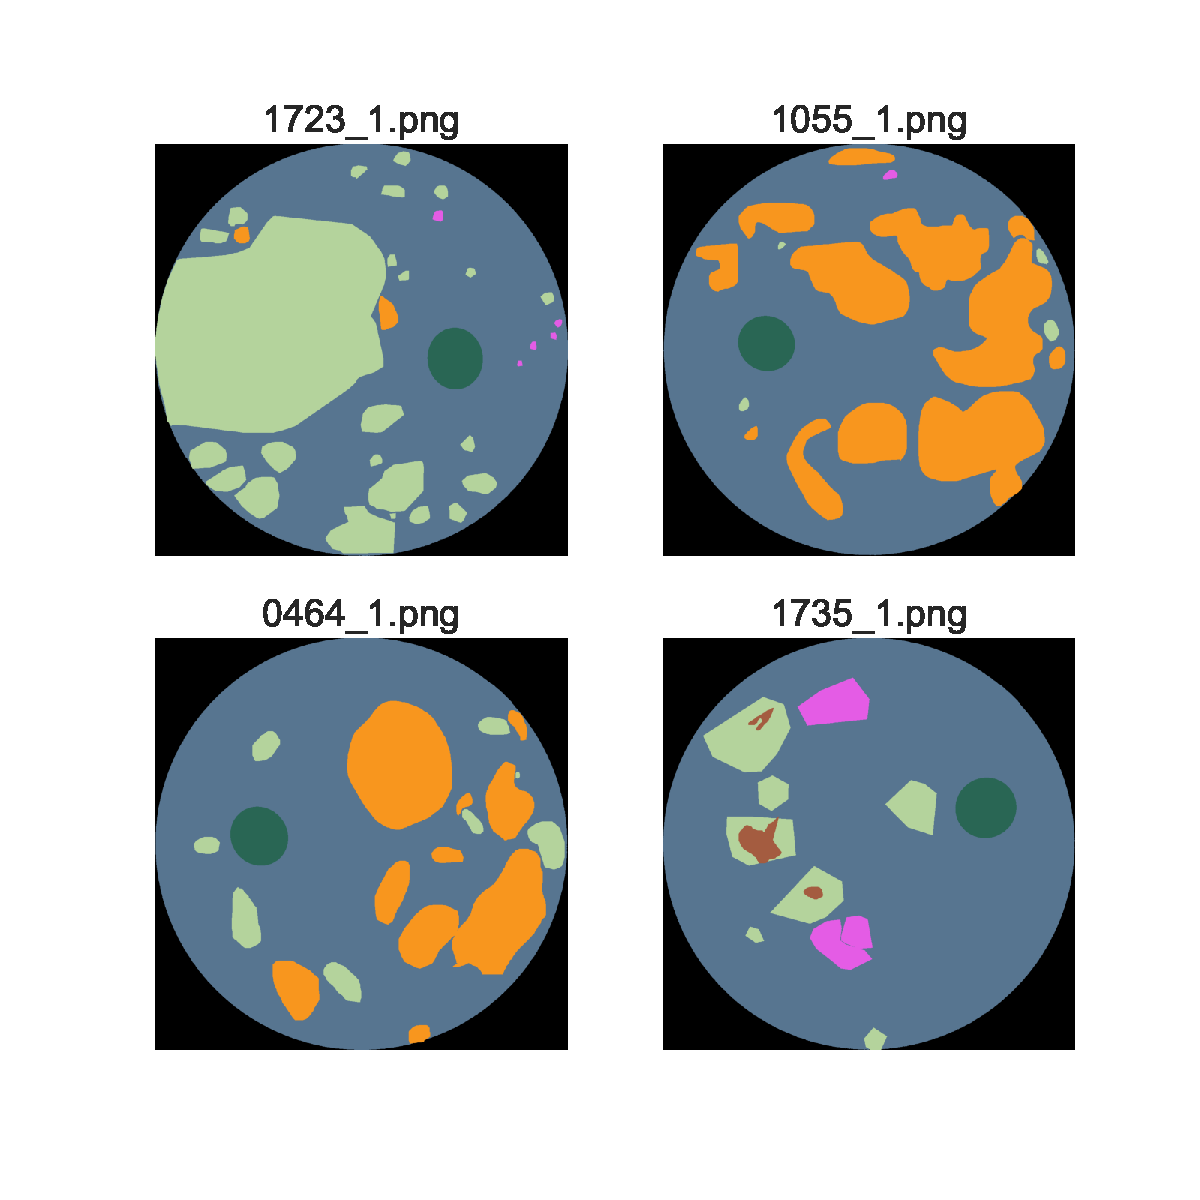
\includegraphics[width=\linewidth]{datasets/figs/fgadr_bad_sample.pdf}
        \caption{Sample of images from batch 1.}
        \label{fig:fgadr_bad_sample}
    \end{subfigure} %
    \begin{subfigure}{0.45\textwidth}
        \centering
        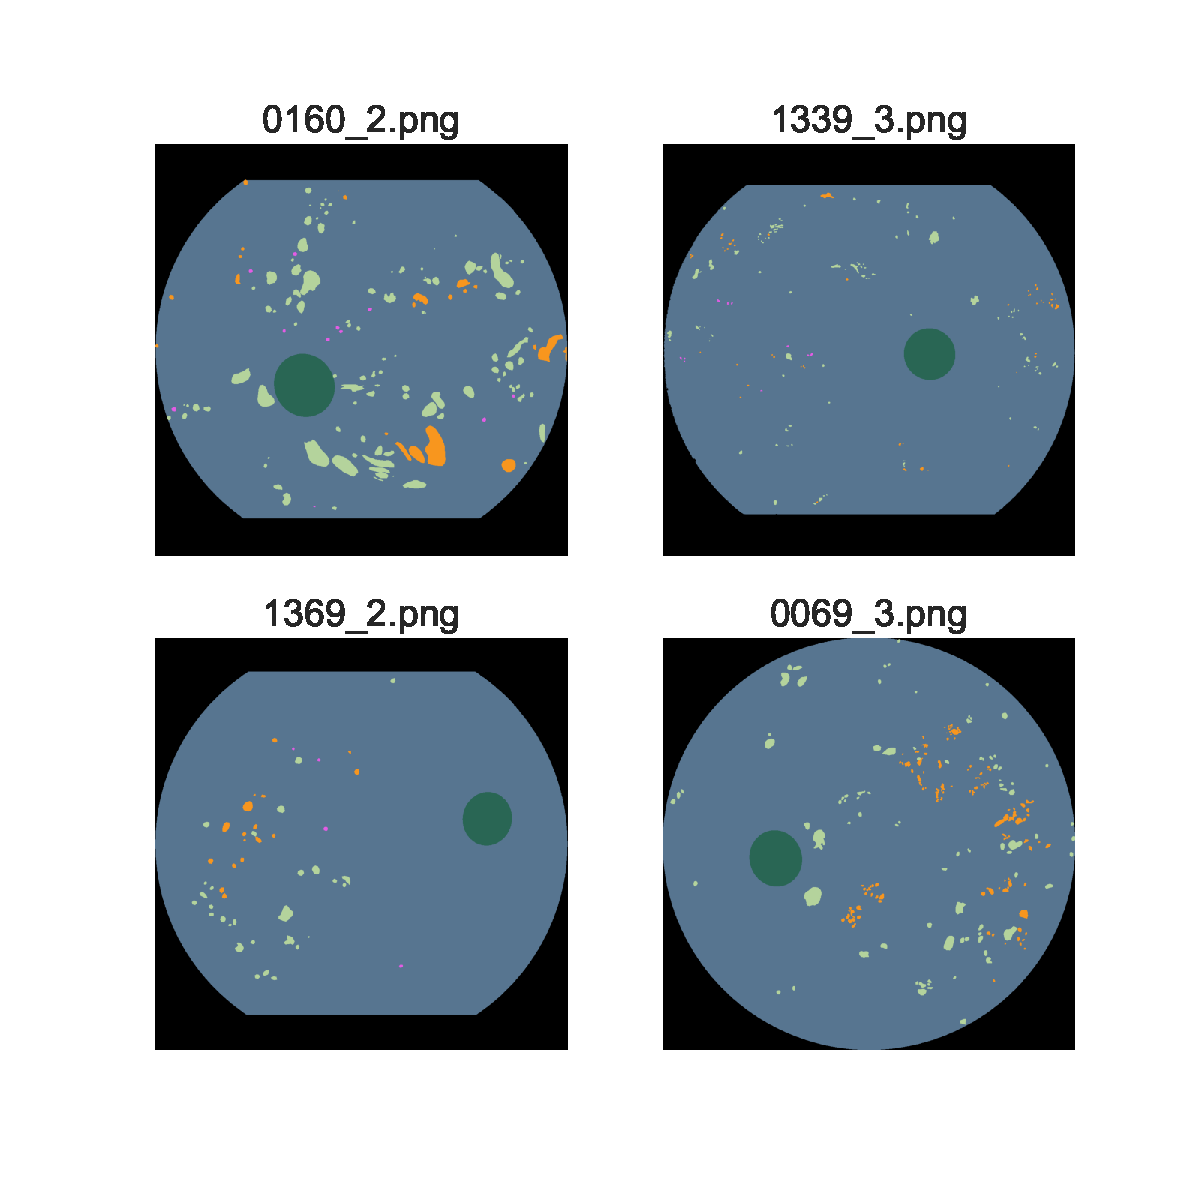
\includegraphics[width=\linewidth]{datasets/figs/fgadr_good_sample.pdf}
        \caption{Sample of images from batches 2 and 3.}
        \label{fig:fgadr_good_sample}
    \end{subfigure}
    \caption{Comparison of annotator bias between batches.}
    \label{fig:fgadr_good_bad}
\end{figure}

Interestingly, a visual examination of the annotations reveals a number of samples which are incongruously annotated compared to the other samples, likely due to annotator bias.
These coarsely annotated files all share a file suffix, following the pattern \lstinline{XXXX_1.png}, a selection of these are shown in \Cref{fig:fgadr_good_bad}.
While not entirely clear from the dataset's descriptor paper, this may indicate the grader, hospital, or something else.
This suffix value can be one of \lstinline{1}, \lstinline{2}, or \lstinline{3}, and we'll refer to this number as the ``batch''.
Apart from the style of annotation, another difference is that this group of files do not have the top and bottom section of the retina cropped, while the other groups have a mix.
One way of removing this bias would be to exclude all 1000 images which contain this suffix. 
However, this is not viable for three reasons: first, this batch makes up over half of the dataset so we would be drastically limiting the amount of available data; secondly, not all of these images suffer from coarse annotations; and finally, this batch represents the entirety of images with grades 0, 1, and 2, removing them would heavily imbalance our data.
Instead, we manually review each of the images in this batch and list those that are determined to be ``too coarse'' (by a non-expert and subjective measure).
We call this the ``FGADR exclusion list'', and can be found in \Cref{sec:fgadr_excl}.

\begin{figure}[h]
    \centering
    \begin{subfigure}{0.45\textwidth}
        \centering
        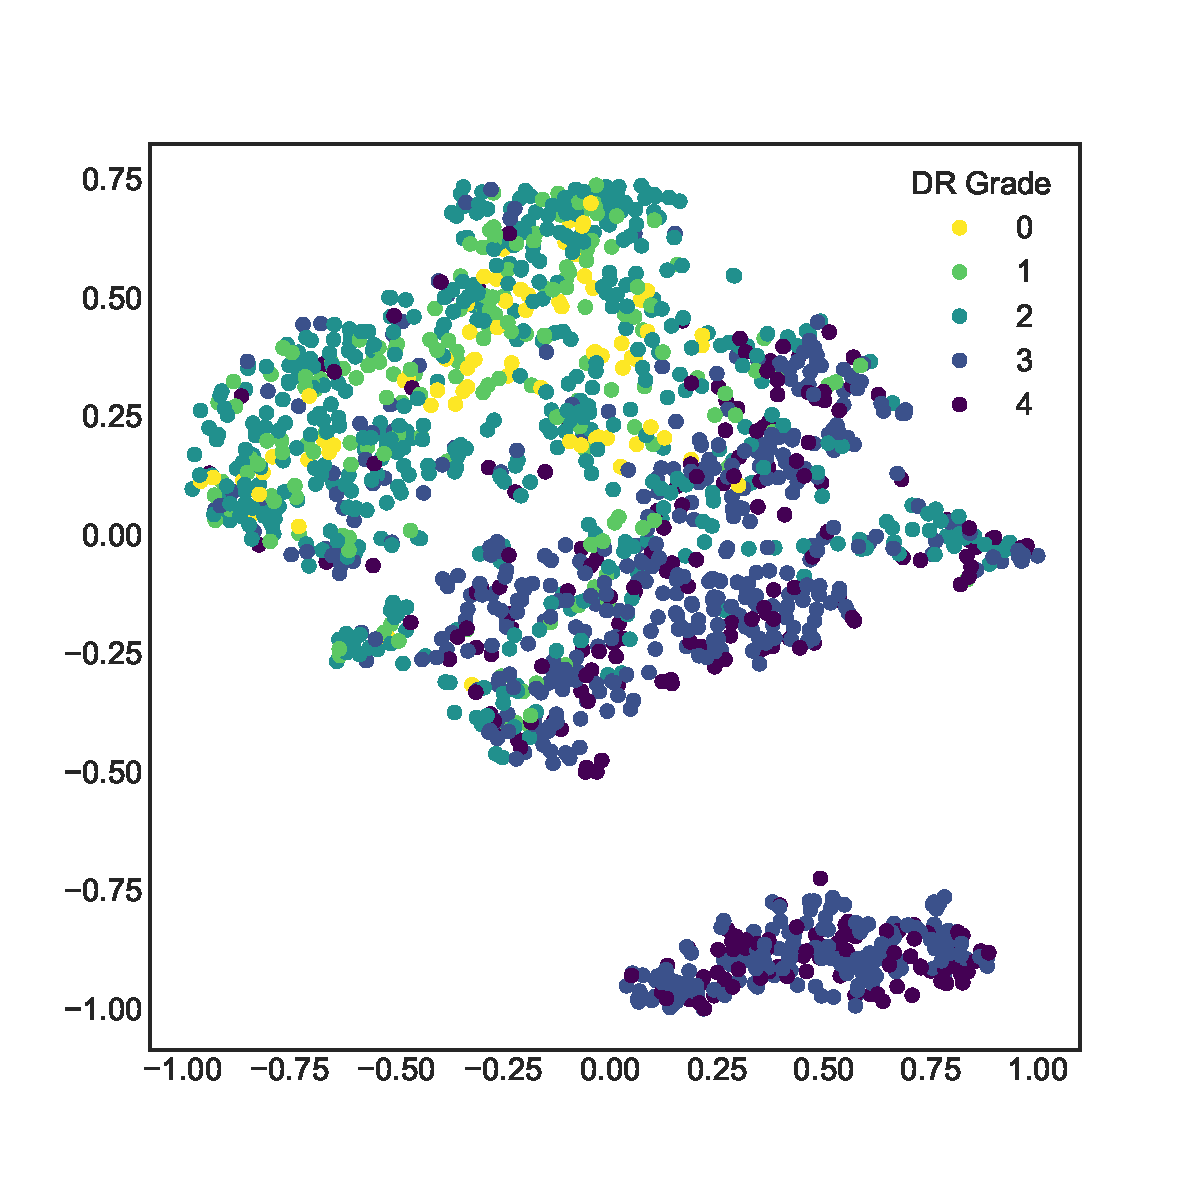
\includegraphics[width=\linewidth]{datasets/figs/fgadr_label_tsne.pdf}
        \caption{Coloured by DR severity grade.}
        \label{fig:fgadr_tsne_grade}
    \end{subfigure} %
    \begin{subfigure}{0.45\textwidth}
        \centering
        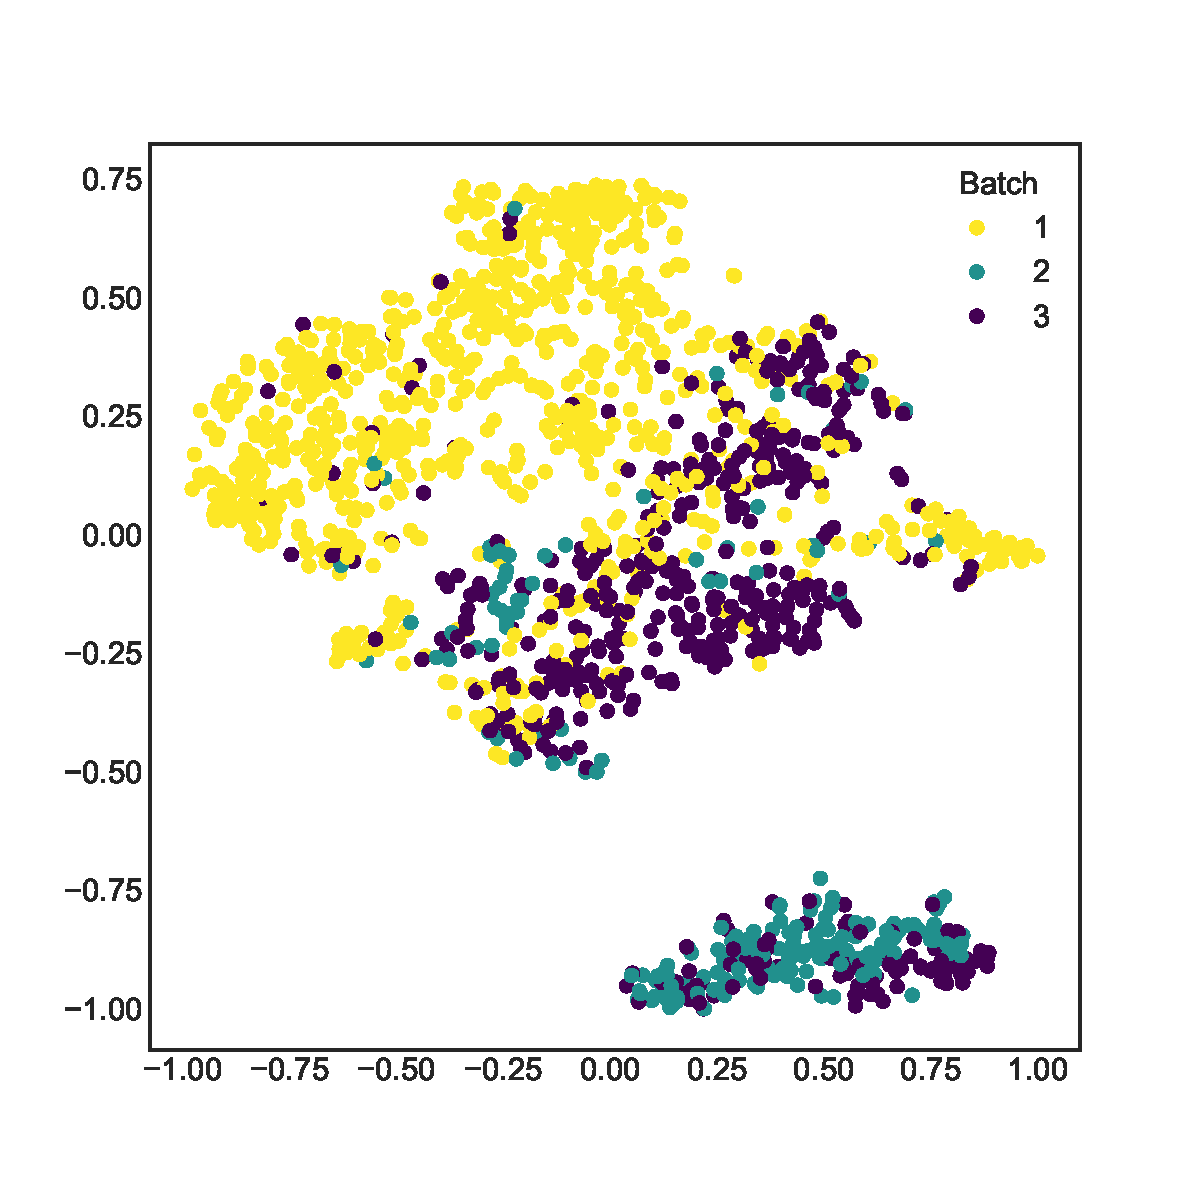
\includegraphics[width=\linewidth]{datasets/figs/fgadr_batch_tsne.pdf}
        \caption{Coloured by batch number.}
        \label{fig:fgadr_tnse_grader}
    \end{subfigure}
    \caption{t-SNE applied to feature vectors extracted from ResNet-50 trained on FGADR labels.}
    \label{fig:fgadr_tsne}
\end{figure}

To deepen our understanding the relationships present in the data, we can apply a dimensionality reduction technique such as t-SNE to create a visual representation which may reveal underlying patterns.
We use the ResNet-50 network as a feature extractor by training it to predict the DR grade of semantic labels from the FGADR dataset.
Note that, while pre-trained networks (on datasets like ImageNet) are commonly used for feature extraction, we decided to train from scratch since our data domain bears little resemblance to those used to train general-purpose networks.
Once trained, we can then extract the learned feature vectors from the layer immediately prior to the final fully-connected layer.
During training, the network was able achieve to 0.86 accuracy on the training set, and 0.53 accuracy on the validation set, which is an indication that there is at least some predictive power in the images.
This relationship is confirmed visually by examining the result of running t-SNE on these feature vectors, shown in \Cref{fig:fgadr_tsne_grade}.
There is a distinct separation between images which have a high DR severity and low DR severity, even if the clusters are not particularly well-defined.

However, given the discrepancy between image batches we identified earlier, it's possible that the features being calculated are more to do with the batch.
To explore this possibility, we plot the same t-SNE components, but this time colour the points by the batch number, depicted in \Cref{fig:fgadr_tnse_grader}.
There are two factors at play here: difference in features between batches, and grade distribution.
For instance, as mentioned earlier, all images with grade 0, 1, and 2 belong to batch 1, and this is reflected in the dimensionality reduction.
The isolated cluster in the lower-right corner is an example of the latter factor, and consists of images which have the top and bottom sections cropped.
While interesting, we expect that there is sufficient diversity within the dataset, and the final training dataset will further combine multiple other datasets, and hence does not pose an obstacle.

\section{IDRiD}

\begin{figure}[h]
    \centering
    \begin{subfigure}{0.45\textwidth}
        \centering
        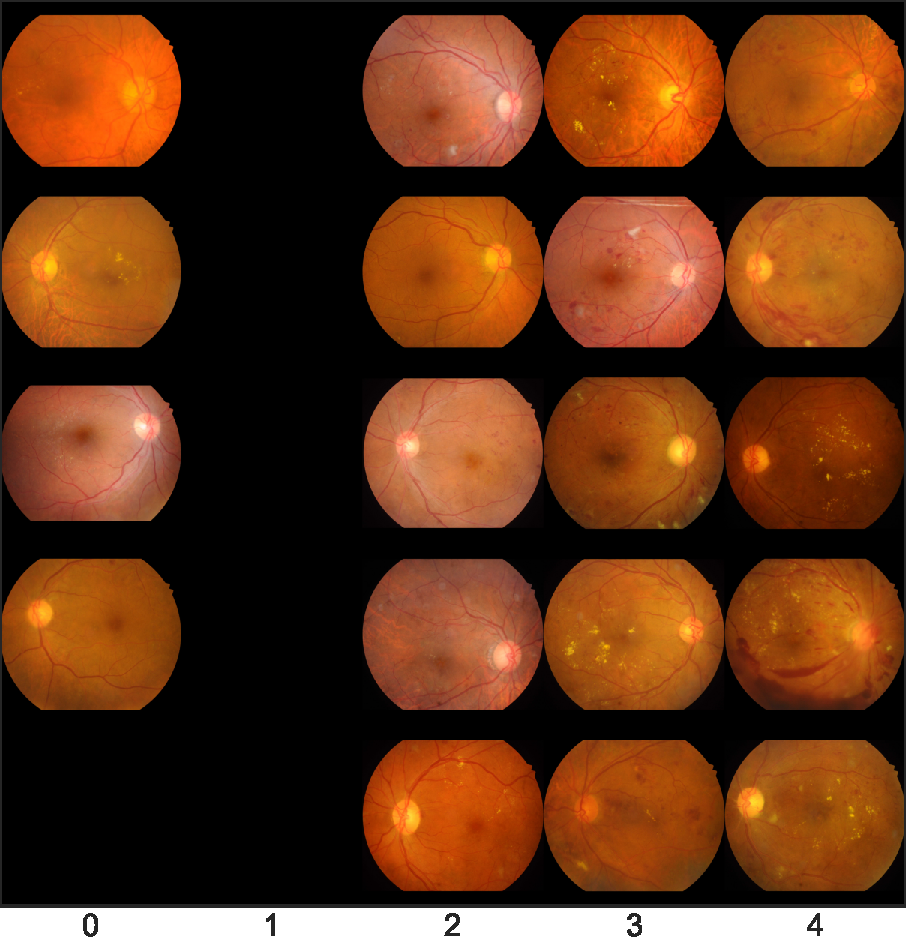
\includegraphics[width=\textwidth]{datasets/figs/idrid_real_sample.pdf}
        \caption{Retina fundus images.}
        \label{fig:idrid_sample_real}
    \end{subfigure} %
    \begin{subfigure}{0.45\textwidth}
        \centering
        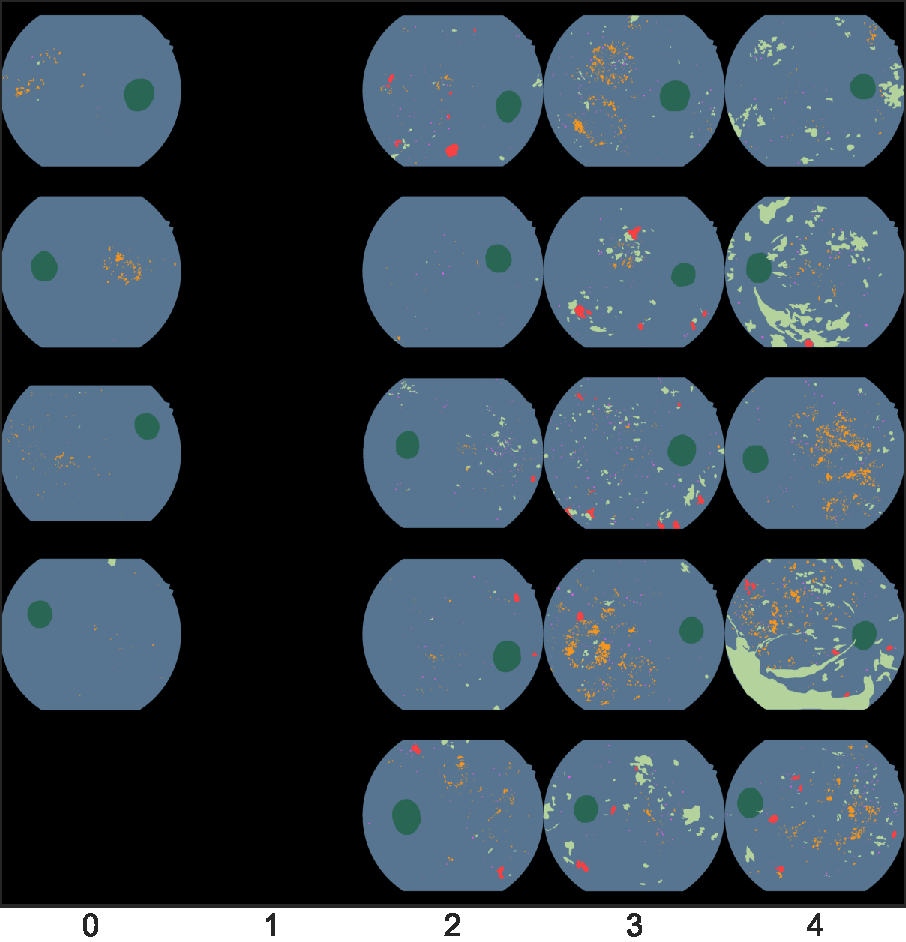
\includegraphics[width=\textwidth]{datasets/figs/idrid_label_sample.pdf}
        \caption{Corresponding semantic labels.}
        \label{fig:idrid_sample_label}
    \end{subfigure}
        \caption{A sample of images from the IDRiD dataset and accompanying manual semantic annotations. Columns from left to right correspond to \emph{inferred} DR grades 0 through 4.}
    \label{fig:idrid_sample}
\end{figure}

The Indian Diabetic Retinopathy Image Dataset (IDRiD) \cite{Porwal2018} was initially released in 2018 as part of the ``Diabetic Retinopathy: Segmentation and Grading Challenge'' held at ISBI-2018.
Similarly to the FGADR dataset, the IDRiD dataset also consists of multiple subsets.
The first subset, aimed at training segmentation models, contains 81 retinal fundus images with varying levels of DR, each of which are accompanied by pixel-level annotations for the optic disc, microaneurysms, soft exudates, hard exudates, and haemorrhages.
Unlike FGADR, annotations for neovascularization, intraretinal microvascular abnormalities, or image-level DR grades for these images are not provided.
The second subset, aimed at training classification models, consists of 516 images annotated with DR severity grades only.
The images in the second subset are exclusive with those in the first subset, and thus none of the images in this dataset contain both image-level and pixel-level annotations, as in the FGADR dataset.
Each image has a resolution of $4288\times 2848$.

To obtain inferred DR grades on this dataset for weakly-supervised learning, we train a model to predict the DR grade from the retinal fundus images.
This method is given in greater detail in \Cref{sec:grade_inference}.
The distribution of the resulting grades has relatively few grade 0s since all images exhibit some form of DR.
There are no grade 1 images, which can likely be attributed tsto bias in the grade inference network.

\section{E-Ophtha}

\begin{figure}[h]
    \centering
    \begin{subfigure}{0.45\textwidth}
        \centering
        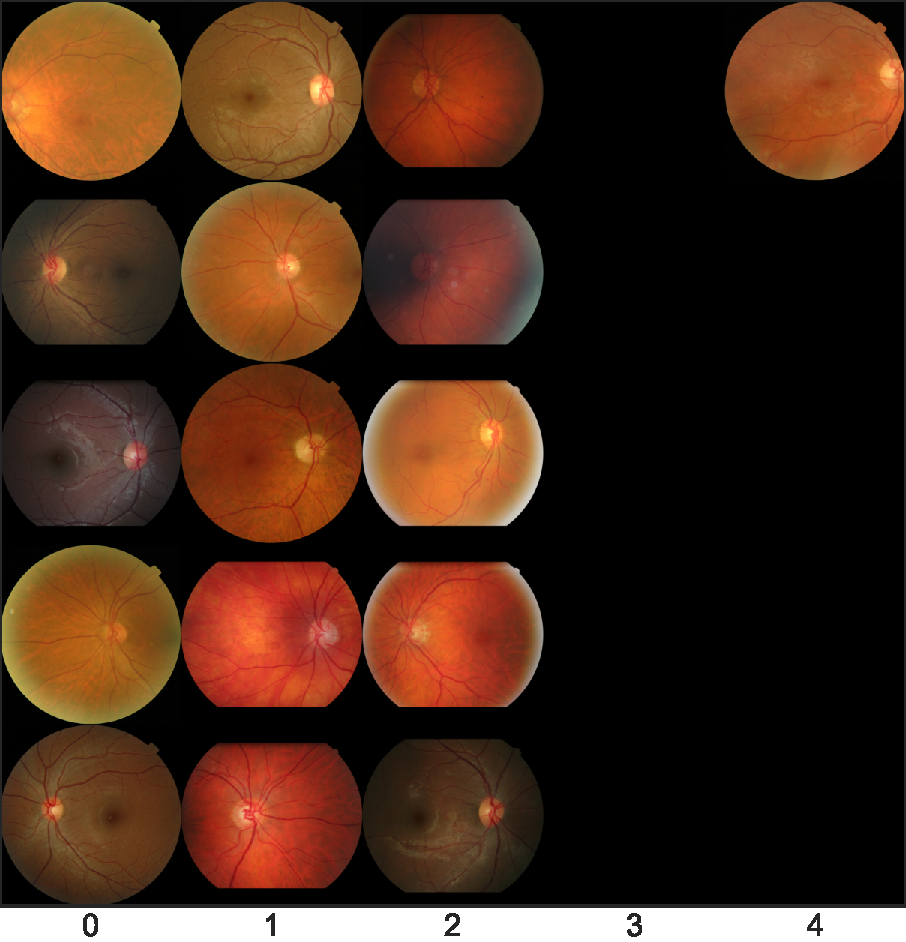
\includegraphics[width=\textwidth]{datasets/figs/eophtha_real_sample.pdf}
        \caption{Retina fundus images.}
        \label{fig:eophtha_sample_real}
    \end{subfigure} %
    \begin{subfigure}{0.45\textwidth}
        \centering
        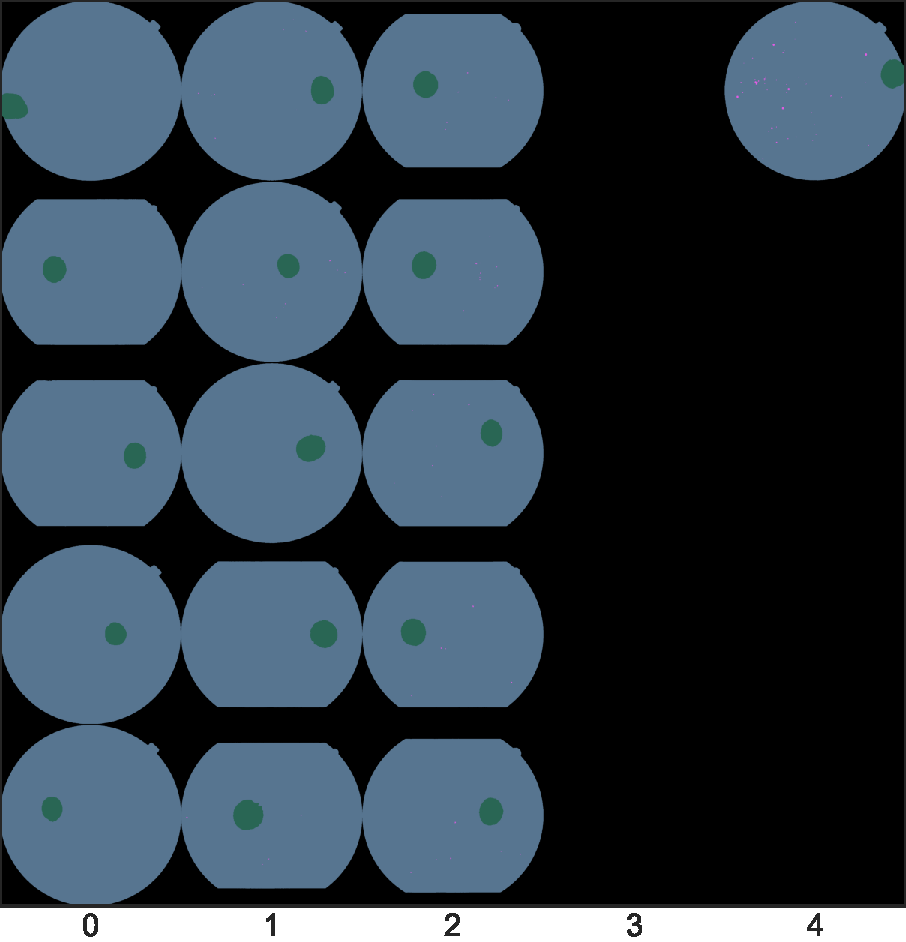
\includegraphics[width=\textwidth]{datasets/figs/eophtha_label_sample.pdf}
        \caption{Corresponding semantic labels.}
        \label{fig:eophtha_sample_label}
    \end{subfigure}
        \caption{A sample of images from the e-ophtha dataset and accompanying manual semantic annotations. Columns from left to right correspond to \emph{inferred} DR grades 0 through 4.}
    \label{fig:eophtha_sample}
\end{figure}

The e-ophtha\footnote{Sometimes (mis-)spelled ``e-optha'' in the dataset files.} \cite{eoptha} dataset was released in 2013 and contains pixel-level annotations for exudates (it is not specified whether these are hard or soft exudates) and microaneurysms.
The images are provided as two subsets: e-ophtha-EX and e-ophtha-MA, each of which also contains a number of ``healthy'' images which do not exhibit the respective lesion (but may have other lesions).
In total, 26 images are annotated with exudates only, 128 are annotated with microaneurysms only, 21 are annotated with both, and 269 images are not annotated with any kind of lesion.
Image resolution varies from $1440 \times 960$ to $2544 \times 1696$.
A sample of images is shown in \Cref{fig:eophtha_sample}; notice how the density of annotations here is much less than those in the FGADR and IDRiD datasets.
This can be largely attributed to the fact that fewer lesion types are annotated, as well as the annotations simply being more fine-grained.
For this dataset, instead of manually annotating optics discs, we infer them using a model as described in \Cref{sec:optic_disc_inference}.

\section{EyePACS}

The EyePACS dataset was first released in 2015 for the Kaggle Diabetic Retinopathy Detection challenge \cite{eyepacs}. 
It is the largest dataset of retinal fundus images for the purpose of grading the severity of diabetic retinopathy, consisting of 88,702 images graded from 0 to 4.
Pixel-level annotations are not provided.
Despite the large volume of data, the quality of images is highly variable, particularly compared to the other datasets we are using, which appear to be more closely curated.
Moreover, the labels are highly imbalanced, with 73.5\% of images being grade 0, and just 2.0\% being grade 4.
For the purpose of the original competition, public/private training and testing sets are provided, but we disregard these and instead create our own subsets.

\section{Data Split}

\begin{figure}[h]
    \centering
    \begin{subfigure}{0.3\textwidth}
        \centering
        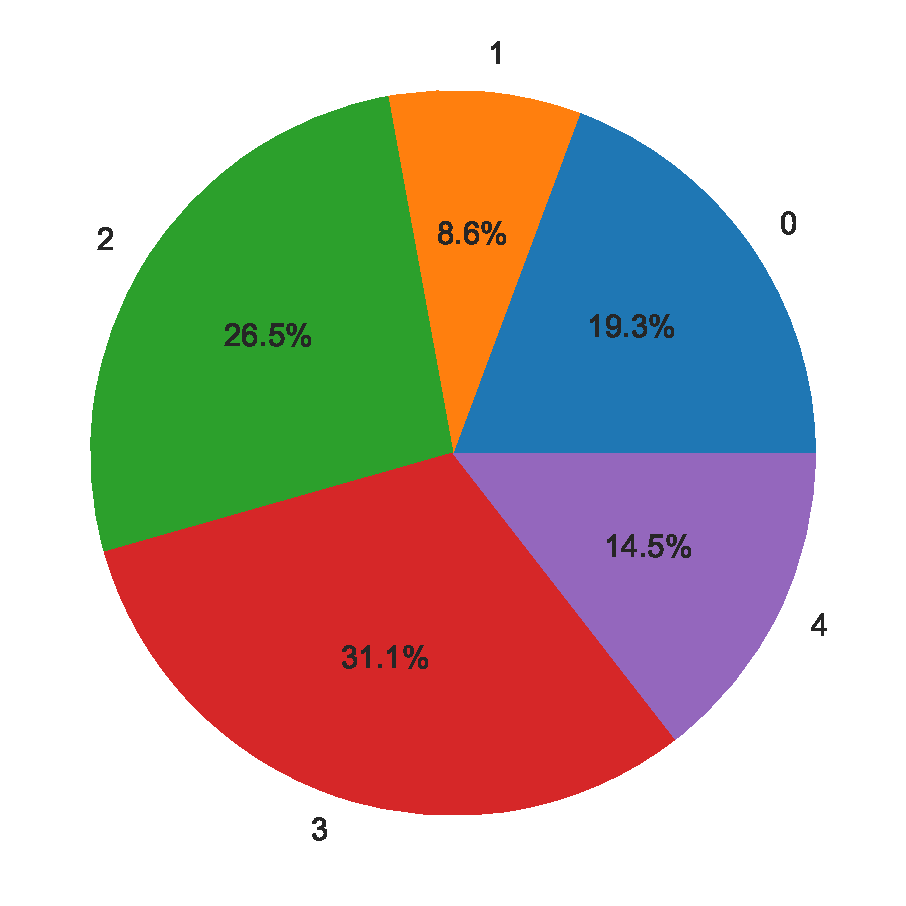
\includegraphics[width=\textwidth]{datasets/figs/combined_grade_dist.pdf}
        \caption{Segmentation dataset.}
        \label{fig:segmentation_grade_dist}
    \end{subfigure}
    \begin{subfigure}{0.3\textwidth}
        \centering
        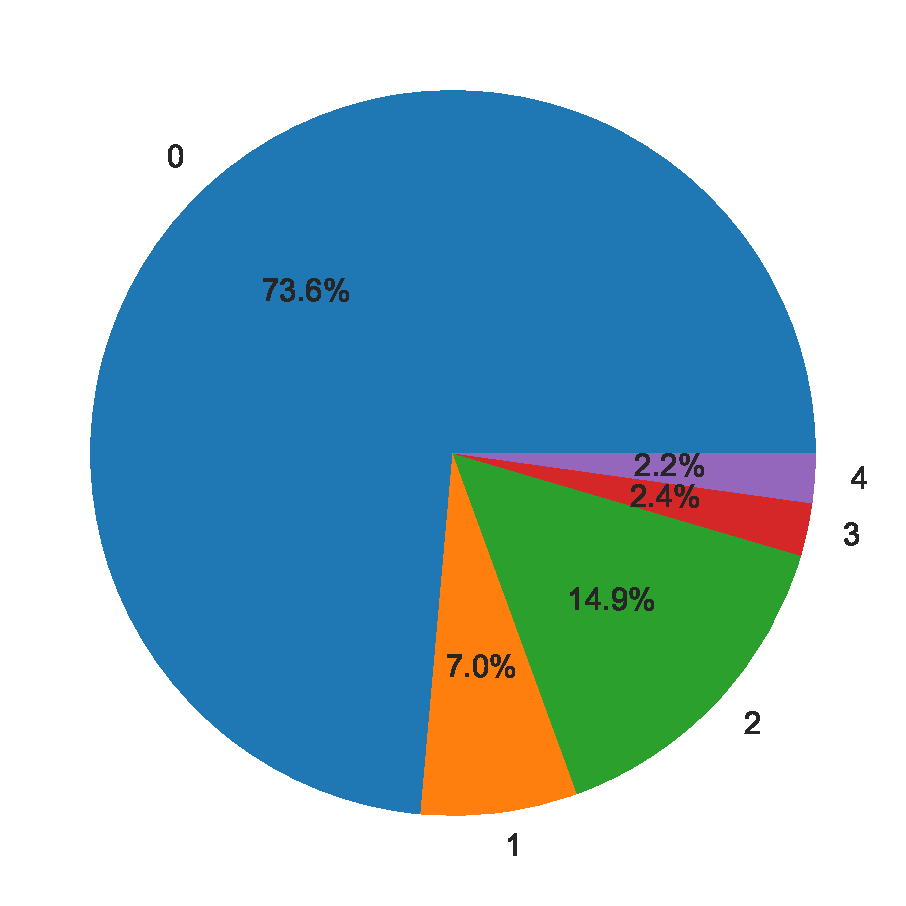
\includegraphics[width=\textwidth]{datasets/figs/eyepacs_grade_dist.pdf}
        \caption{EyePACS dataset.}
        \label{fig:eyepacs_grade_dist}
    \end{subfigure}
    \begin{subfigure}{0.3\textwidth}
        \centering
        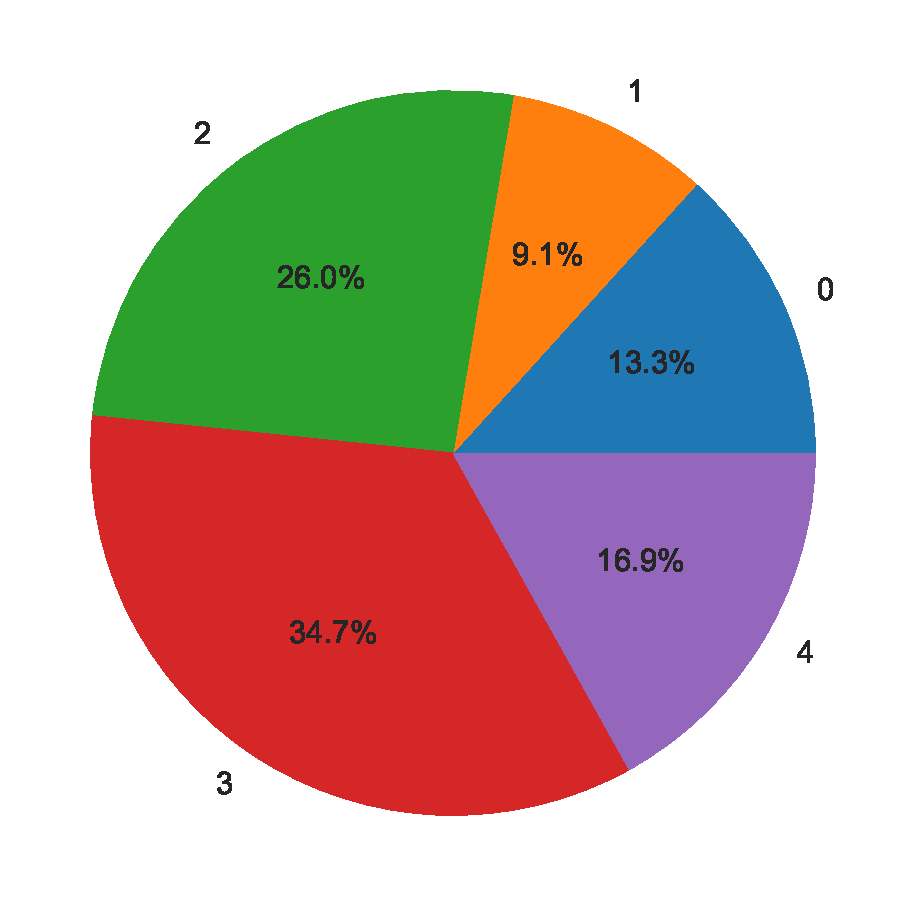
\includegraphics[width=\textwidth]{datasets/figs/grading_grade_dist.pdf}
        \caption{Grading dataset.}
        \label{fig:grading_grade_dist}
    \end{subfigure}
    \caption{Distribution of DR grades in various datasets.}
    \label{fig:combined_grade_dist}
\end{figure}

We combine the FGADR, IDRiD, and e-ophtha datasets to train our semantic label generation models.
In order to prevent data leakage, we randomly separate out (and fix) training, validation, and test sets, according to \Cref{tab:label_split}.
We train all generative models on the training set, compare models using the validation set, and use the test set for the final evaluation.

\begin{table}[h]
    \centering
    \begin{tabular}{lrrrrr}
        \toprule
        \multirow{2}{*}{Subset} & \multirow{2}{*}{Proportion} & \multicolumn{4}{c}{\# Images} \\
        \cmidrule{3-6}
         & & FGADR & IDRiD & e-ophtha & Total \\
        \midrule
        Training & 0.80 & 1194 & 61 & 352 & 1607 \\
        Validation & 0.10 & 151 & 13 & 37 & 201 \\
        Test & 0.10 & 149 & 7 & 45 & 201 \\
        \midrule
        Total & 1.00 & 1494 & 81 & 434 & 2009 \\
        \bottomrule
    \end{tabular}
    \caption{Data split for segmentation data.}
    \label{tab:label_split}
\end{table}

For the EyePACS training set we simply take a training and test split, according to \Cref{tab:eyepacs_split}.

\begin{table}[h]
    \centering
    \begin{tabular}{lrr}
        \toprule
        Subset & Proportion & \# Images \\
        \midrule
        Training & 0.80 & 70,961 \\
        Test & 0.20 & 17,741 \\
        \midrule
        Total & 1.00 & 88,702 \\
        \bottomrule
    \end{tabular}
    \caption{Data split for the EyePACS dataset.}
    \label{tab:eyepacs_split}
\end{table}

We also create a small grading set by combining samples from FGADR \emph{Seg-set} and the IDRiD grading set, shown in \Cref{tab:grading_split}.
We use the same FGADR training set from the segmentation split to avoid data leakage.
This is not a concern for the IDRiD dataset since the IDRiD segmentation and grading datasets are mutually exclusive.

\begin{table}[h]
    \centering
    \begin{tabular}{lrrrr}
        \toprule
        \multirow{2}{*}{Subset} & \multirow{2}{*}{Proportion} & \multicolumn{3}{c}{\# Images} \\
        \cmidrule{3-5}
         & & FGADR & IDRiD & Total \\
        \midrule
        Training & 0.80 & 1194 & 412 & 1606 \\
        Validation & 0.10 & 151 & 52 & 203 \\
        Test & 0.10 & 149 & 52 & 201  \\
        \midrule
        Total & 1.00 & 1494 & 516 & 2010  \\
        \bottomrule
    \end{tabular}
    \caption{Data split for grading data.}
    \label{tab:grading_split}
\end{table}

\section{Other Datasets}

Other datasets for diabetic retinopathy related tasks are available, but were inappropriate for our use case.
Specific reasons are given below:
\begin{description}
    \item[DiaRetDB0] \hfill \\ Released in 2006 as part of the ImageRet\footnote{\url{https://www.it.lut.fi/project/imageret}} project.
    DiaRetDB0 does not have pixel-level annotations, only image-level annotations labelling the presence of lesions.
    DiaRetDB1 and DiaRetDB1 v2 were also released by the ImageRet project.
    \item[DiaRetDB1] \hfill \\ Contains 89 images at a resolution of $1500\times 1152$, 84 of which show signs of DR and five which are healthy.
    Images are accompanied by pixel-wise labels for hard exudates, soft exudates, microaneurysms, and ``red small dots'' -- which we interpret as haemorrhages. 
    Labels are not provided for neovascularization or intraretinal microvascular abnormalities, nor are image-level DR grades.
    Interestingly, each image was annotated independently by four different experts, and a confidence level was provided for each marking.
    Unfortunately, after running some experiments, we determined that the annotations are too coarse to be used as segmentation maps.
    However, we still collected manual optic disc annotations for these images, also provided in \Cref{sec:od}.
    \item[DiaRetDB1 v2] \hfill \\ Contains the same data as DiaRetDB1 but in a more flexible data format.
    \item[DRIVE] \hfill \\ Contains 40 images with pixel-level segmentations for vessels only.
    \item[CHASE\_DB1] \hfill \\ Contains 28 images with pixel-level segmentations for vessels only.
    \item[STARE] \hfill \\ Contains 400 images with pixel-level segmentations for vessels only.
    \item[DRISHTI-GS] \hfill \\ Contains 101 images with pixel-level segmentations for the optic disc only.
    \item[Messidor] \hfill \\ Contains 1200 images graded by their risk of diabetic macular oedema, instead of diabetic retinopathy.
\end{description}

\section{Data Pre-Processing}

\begin{figure}[h]
    \centering
    \begin{subfigure}{0.45\textwidth}
        \centering
        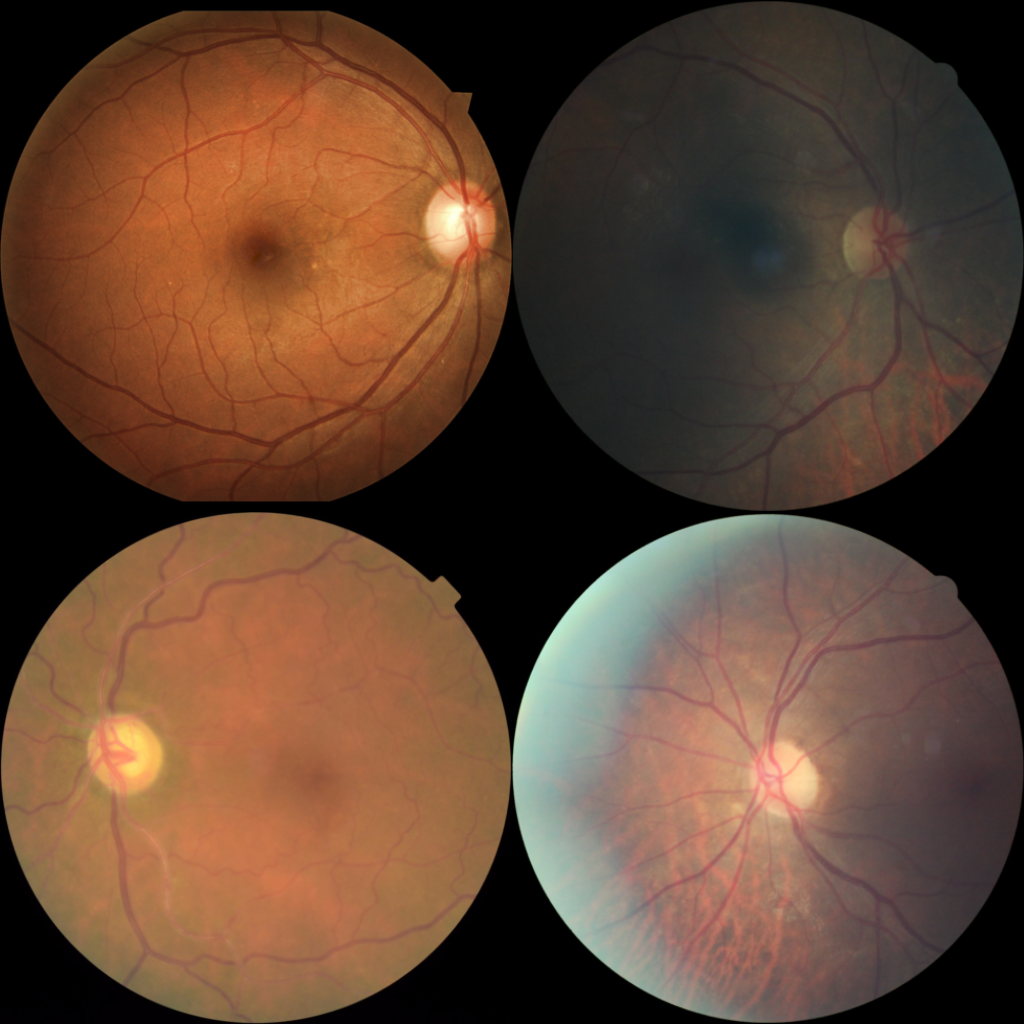
\includegraphics[width=\linewidth]{datasets/figs/eyepacs_before.png}
    \end{subfigure} %
    \begin{subfigure}{0.45\textwidth}
        \centering
        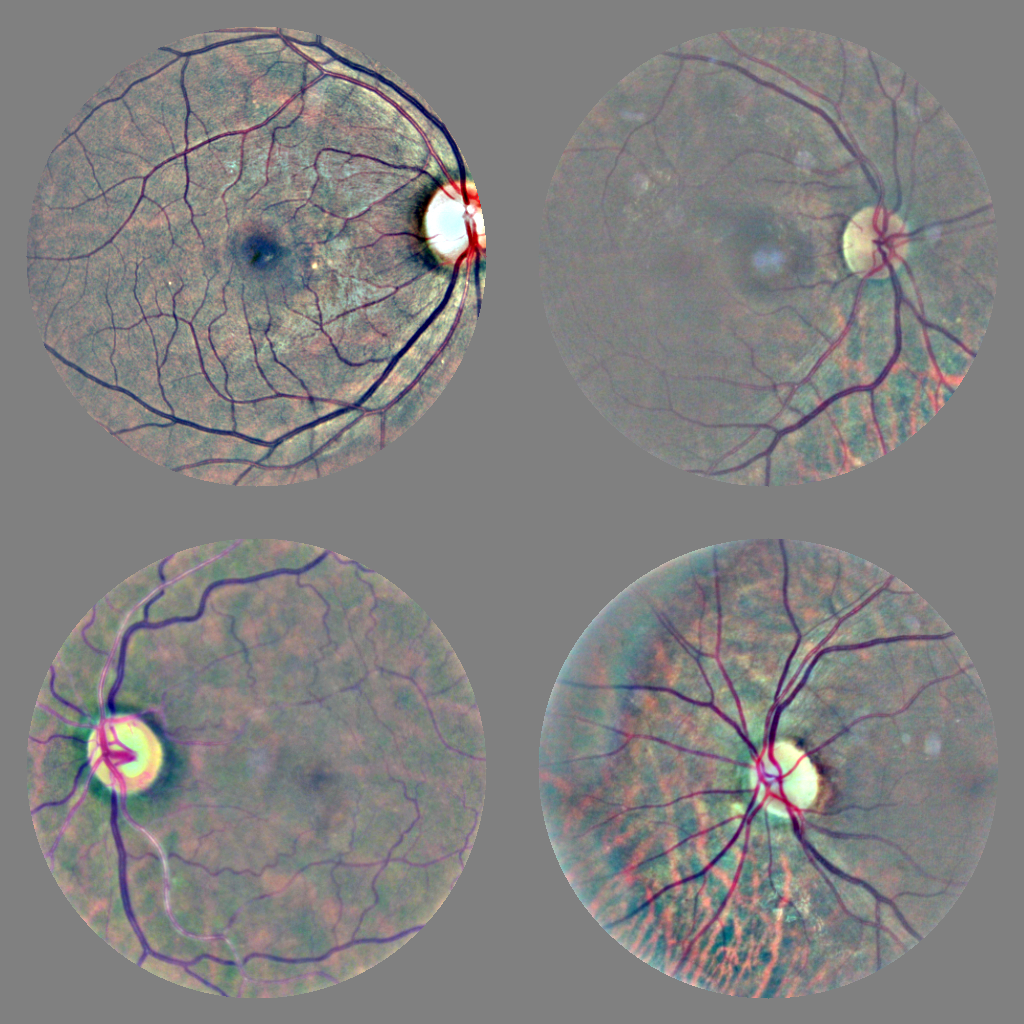
\includegraphics[width=\linewidth]{datasets/figs/eyepacs_after.png}
    \end{subfigure}
    \caption{Before (left) and after (right) illumination correction.}
    \label{fig:preprocess_before_after}
\end{figure}
To ensure image size and retina positioning is uniform across all images, we perform the following steps:
\begin{enumerate}
    \item Extract a mask for the retinal fundus boundary by performing a binary threshold.
    \item Draw a bounding box around this boundary.
    \item Crop around the bounding box so that the retina is now centred and fills the image.
    \item Pad to square.
    \item Resize to $1280 \times 1280$.
\end{enumerate}
To further correct for illumination differences between retina photographs, we borrow image processing techniques from Benjamin Graham \cite{benjamingraham}, winner of the 2015 Kaggle Diabetic Retinopathy Challenge\footnote{\url{ https://www.kaggle.com/c/diabetic-retinopathy-detection}}:
\begin{enumerate}
    \setcounter{enumi}{5}
    \item Subtract the local average.
    \item Clip the radius to remove boundary effects.
\end{enumerate}
Each pixel-annotated dataset provides binary masks for each lesion class.
The segmentation masks for each class are combined into a single-channel image, where the discrete value of each pixel encodes its label.
That is, each retina semantic label with height $H$ and width $W$ is represented as an image $M \in \mathbb{L}^{H\times W}$ where $\mathbb{L} = \{ 0, 1, 2, 3, 4, 5, 6, 7, 8 \}$, ensuring that every pixel belongs to exactly one class.
For clarity, the semantic labels have been mapped to RGB colours according to \Cref{tab:mappings}.

\newcommand{\thiscolor}[1]{\hfill \texttt{\convertcolorspec{named}{#1}{RGB}\RGBcolor (\RGBcolor)} \fcolorbox{black}{#1}{\hspace{2mm}}}

\definecolor{retina}{RGB}{87, 117, 144}
\definecolor{od}{RGB}{41, 102, 84}
\definecolor{ma}{RGB}{228, 92, 229}
\definecolor{he}{RGB}{180, 211, 156}
\definecolor{ex}{RGB}{248, 150, 30}
\definecolor{se}{RGB}{249, 65, 68}
\definecolor{nv}{RGB}{250, 208, 44}
\definecolor{irma}{RGB}{164, 92, 64}
\definecolor{bg}{RGB}{0, 0, 0}

\begin{table}[h]
    \centering
    \begin{tabular}{lcr}
    \toprule
        Label & Value & RGB Colour \\
    \midrule
        Retina & 0 & \thiscolor{retina}\\ 
        Optic Disc & 1 & \thiscolor{od}\\ 
        Microaneurysms & 2 & \thiscolor{ma} \\ 
        Haemorrhages & 3 & \thiscolor{he} \\ 
        Hard Exudates & 4 & \thiscolor{ex} \\ 
        Soft Exudates & 5 & \thiscolor{se} \\ 
        Neovascularization & 6 & \thiscolor{nv} \\ 
        Intraretinal Microvascular Abnormalities & 7 & \thiscolor{irma} \\ 
        Background & 8 & \thiscolor{bg} \\ 
    \bottomrule
    \end{tabular}
    \caption{Semantic label values and colour mappings.}
    \label{tab:mappings}
\end{table}

\section{Grade Inference} \label{sec:grade_inference}

To infer grades, a ResNet-101 network was trained for 20 epochs on the EyePACS dataset, with images pre-processed as detailed in the previous section.
We use this over the smaller grading dataset since the EyePACS dataset contains a much greater volume of data with more diversity.
Images were resized to $512 \times 512$ before being passed through the network. 
Training was done on on one Nvidia GeForce GTX 1080 GPU over 48 hours.
The data was split according to \Cref{tab:eyepacs_split}, and the model was trained with the Adam optimiser, $\alpha=0.001$ and batch size 8.

To accelerate training on such a large dataset, the images were first pre-processed and saved to disk in the HDF5 format, allowing for more efficient data retrieval.
Doing this allowed data to be loaded up to 12.54 times faster (at the cost of storage space).
However, training was largely bottlenecked by GPU processing speed instead of disk I/O, so this did not translate to real-world training improvement.

For data augmentation, we randomly rotate between 0 and 360 degrees, randomly translate by between (-10\%, +10\%) vertically and horizontally, and randomly shear parallel to the x axis in the range (-0.2, +0.2).

\begin{table}[h]
    \centering
    \begin{tabular}{lrrrrr}
        \toprule
        Configuration & Accuracy & Precision & Recall & $F_1$ & $\kappa$ \\
        \midrule
        ResNet-101 & 0.8208 & 0.6574 & 0.3836 & 0.4845 & 0.6309 \\
        \bottomrule
    \end{tabular}
    \caption{Performance of the grade inference model on the EyePACS test set.}
    \label{tab:resnet_results}
\end{table}

We also experimented with test-time augmentation, but did not find that this improved the model's performance, and incurred a significant performance penalty.
The evaluation metrics on the test set are reported in \Cref{tab:resnet_results}.

The trained model can be found in \Cref{sec:models}.

\section{Optic Disc Inference} \label{sec:optic_disc_inference}

To infer optic discs, we train a basic U-Net architecture on the pre-processed retinal fundus images to predict the optic discs provided by the IDRiD dataset and manual annotations collected on the training subset of the FGADR and DiaRetDB1 datasets.
For the FGADR dataset, we include the coarsely annotated images since they have no bearing on the optic disc annotations.
As data augmentation, we apply custom transformations during training to vertically and horizontally flip the images and masks jointly.
Images were resized to $512 \times 512$.

We train using the Adam optimiser with a $\alpha=0.001$ and batch size 8 for 50 epochs on one Nvidia Titan X Pascal GPU for 1 hour and 21 minutes.
The evaluation metrics on the test set are reported in \Cref{tab:od_results}.

\begin{table}[h]
    \centering
    \begin{tabular}{lrrr}
        \toprule
        Configuration & Precision & Recall & $F_1$ \\
        \midrule
        U-Net & 0.9484 & 0.9657 & 0.9561 \\
        \bottomrule
    \end{tabular}
    \caption{Performance of the optic disc inference model on the semantic label test set.}
    \label{tab:od_results}
\end{table}

After inference, there were 11 spurious annotations which had to be corrected manually using the GIMP\footnote{\url{https://www.gimp.org}} image editor.

The trained model can be found in \Cref{sec:od}.
\chapter{Semantic Label Generation} \label{cha:labels}

The main objective of this work is concerned with predicting plausible layouts of retina structures and lesions.
We first approach this by using a GAN to generate semantic labels, trained on manual annotations.
By using a sophisticated generative model, we hope to be able to capture subtle relationships and interactions between the various different retinal structures, which would not be possible with classical data augmentation techniques.
Then we study how a heuristic-based method that samples from existing data in a ``naive'' way compares with the generative models.

In this section, we discuss the unique challenges of this task, and go on to compare three different approaches.

\section{Initial Experiments}

During the initial exploration phase for this task, we began by applying implementations of the most modern GAN designs, such as ContraGAN and StyleGAN.
To do this, we had to modify the generator and discriminator architectures to suit our problem domain, instead of creating RGB images.
Recall our semantic \emph{images} are represented as $M \in \mathbb{L}^{H \times W}$, where $\mathbb{L} = \{0, ..., 9\}$.
To extract the one-hot encoded (w.r.t each pixel) semantic \emph{label} representation, we extract the appropriate labels from this image, to get the desired input $S \in \{ 0, 1 \}^{C \times H \times W}$.
The final layer of the generator becomes a softmax layer, which allows us to interpret each pixel of the output feature map $P \in \mathbb{R}^{C \times H\times W}$ as the probability of that pixel belonging to each class; that is:
\begin{align}
    \forall h \in H, \ \forall w \in W \quad \sum_{c}^C P_{chw} = 1 \text{ and } P_{chw} \geq 0
\end{align}
To recover the semantic image representation, we simply take the arg max of this probability map over the channels.
\begin{align}
    M = \argmax_c P    
\end{align}
This relationship between these representations is depicted graphically in \Cref{fig:semantic_label}.

\begin{figure}[h]
    \centering
    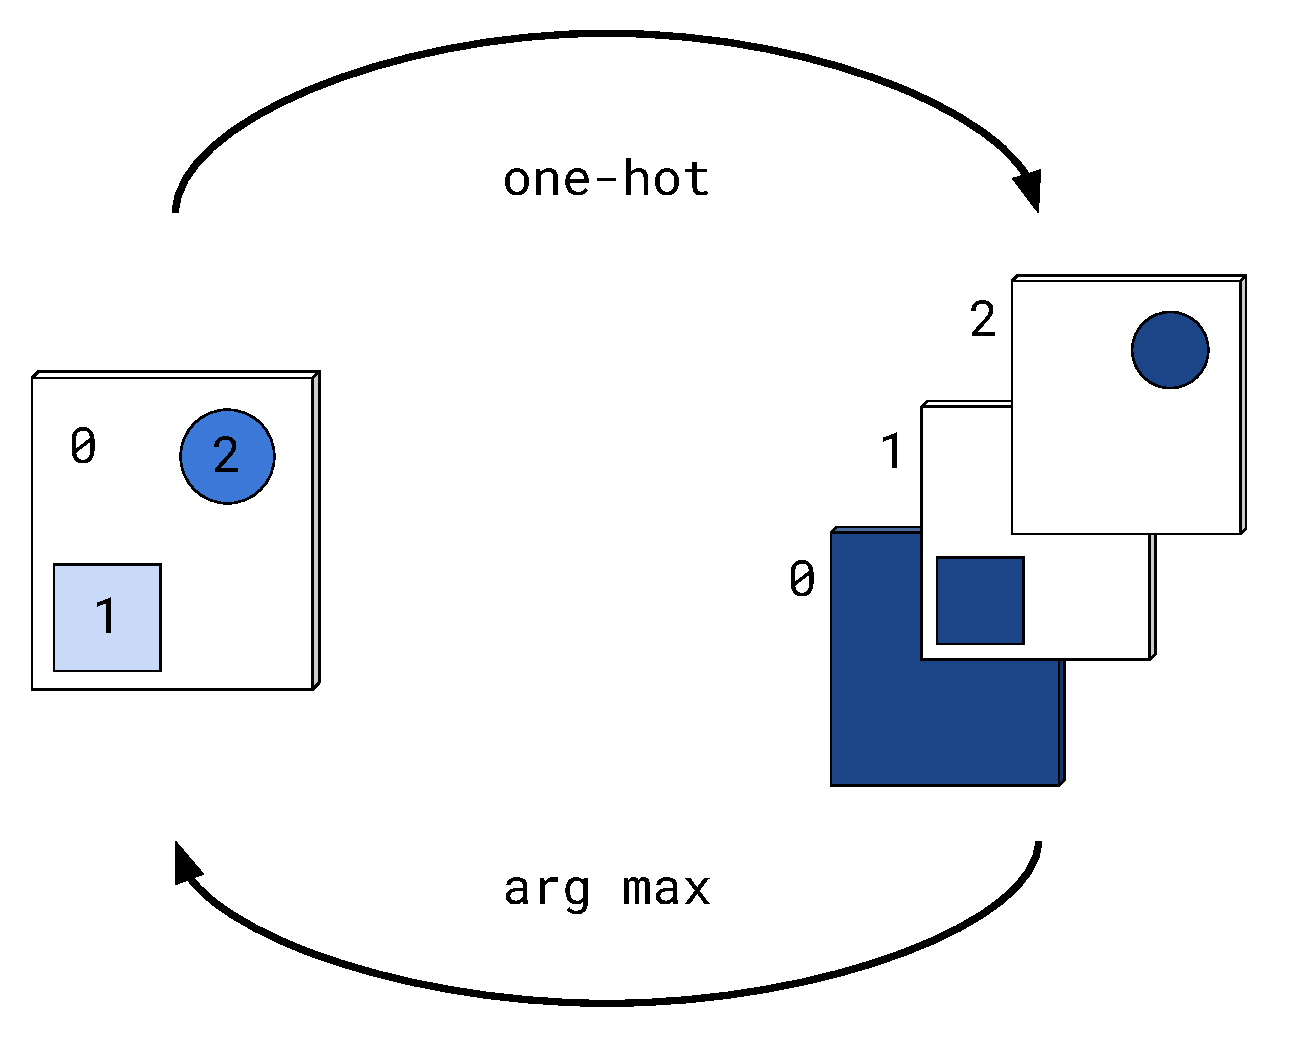
\includegraphics[width=0.5\textwidth]{labels/figs/label-semantics.pdf}
    \caption{Converting between the integer-encoded semantic image and one-hot encoded semantic label representation.}
    \label{fig:semantic_label}
\end{figure}

However, we quickly discovered that these architectures -- primarily concerned with creating high-fidelity, dense, natural, 3-channel images -- collapsed almost immediately, before generating any useful outputs.
In particular, we found that GAN architectures which utilised a ResNet-based discriminator were particularly problematic, even when the capacity of the generator, in terms of the number of parameters, was much greater.
Interestingly, this was not reported by any of the (admittedly limited) existing literature, which largely use architectures based on conventional CNNs.

We theorise that this is because the sparse nature of the semantic labels, coupled with the large number of channels, made it a challenge for the generator to create plausible outputs, while the discriminator learnt very quickly to distinguish real and fake images.
Hence, it was established that we would need to create a bespoke architecture starting from first principles, based on an understanding of what made the task challenging, and how these issues could be mitigated.

\section{ACGAN}

\begin{figure}
    \centering
    \begin{subfigure}{\textwidth}
        \centering
        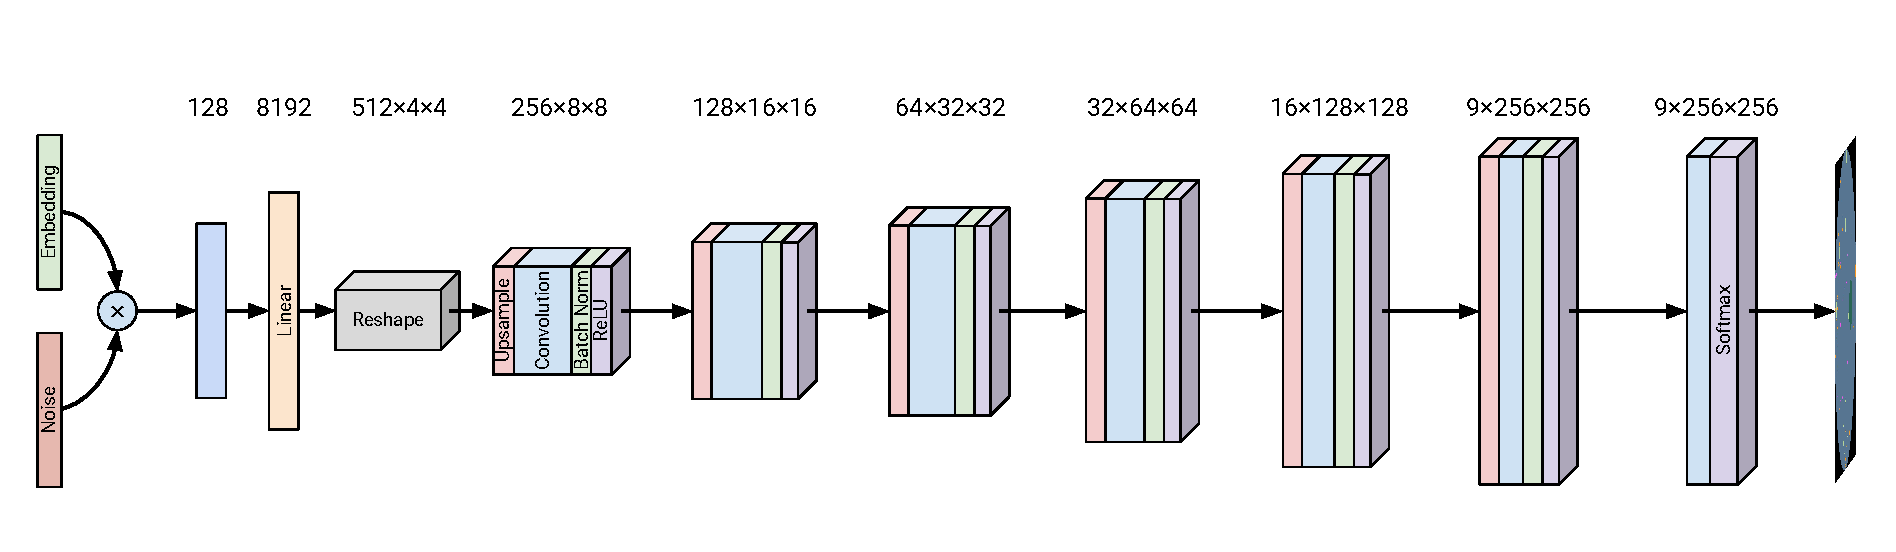
\includegraphics[width=\linewidth]{labels/figs/acgan-generator.pdf}
        \caption{ACGAN generator architecture.}
        \label{fig:acgan_gen}
    \end{subfigure}
    \begin{subfigure}{\textwidth}
        \centering
        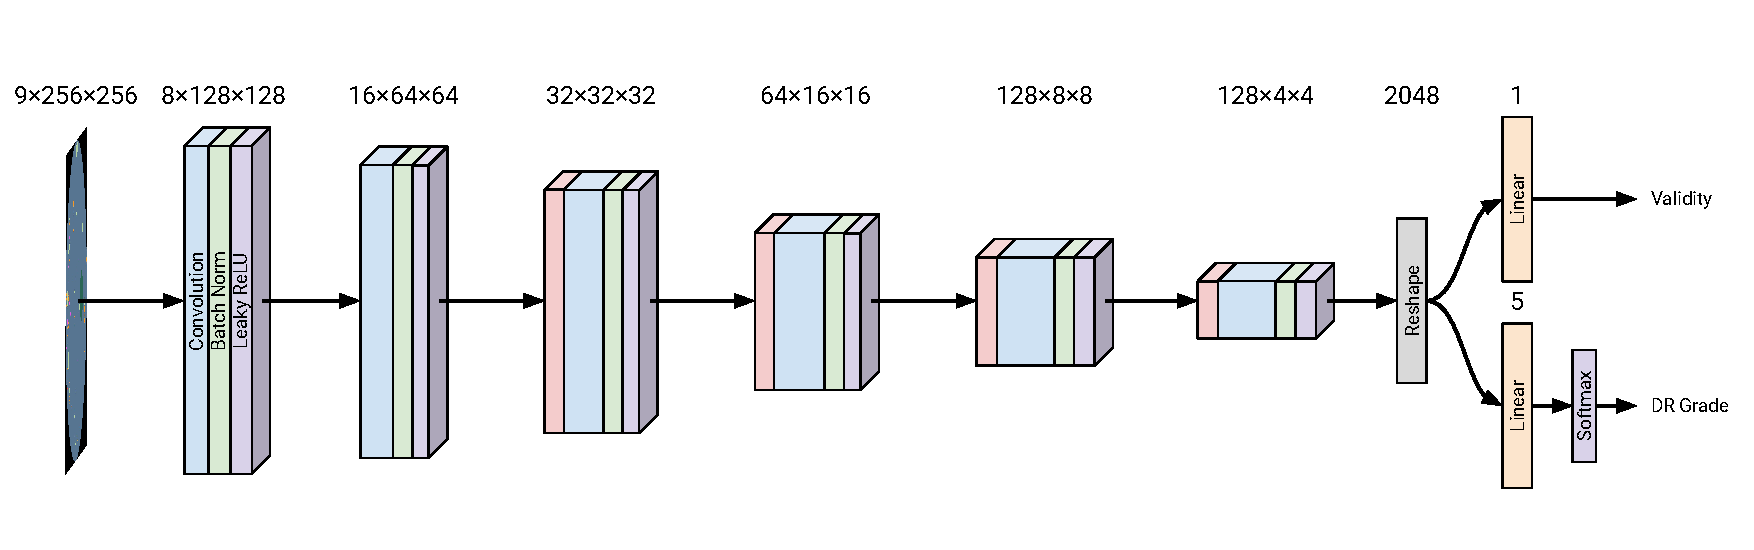
\includegraphics[width=\linewidth]{labels/figs/acgan-discriminator.pdf}
        \caption{ACGAN discriminator architecture.}
        \label{fig:acgan_dis}
    \end{subfigure}
    \caption{ACGAN network architectures.}
    \label{fig:acgan_arch}
\end{figure}

Motivated by this, we designed a DCGAN-based generator and discriminator architecture to generate class-conditioned semantic labels, using auxiliary discriminator losses (ACGAN).
In this conditioning strategy, we add a classification layer to the end of the discriminator which learns to predict the class of the input image \cite{odena2017conditional}.
As the generator attempts to minimise this auxiliary loss, the quality of conditioning will increase.

The generator creates images at a resolution of $256 \times 256$;  we found that attempting to use this architecture to generate images at higher resolutions than this greatly increased instability, since discriminability increases with resolution.
To condition the generator, we take the Hadamard product between the latent noise vector $z$ and the embedded representation of the image class.
Generated images are upsampled to $512 \times 512$ using bilinear interpolation (and then thresholded to valid values) as a post-processing step.

Where this design departs from conventional ACGANs, as presented in their original form, is the asymmetry between the generator capacity (2,672,630 parameters) and discriminator capacity (259,070 parameters).
Limiting the discriminator in terms of both the number of parameters and other training techniques, detailed in the following sections, were key in allowing for stable training.

\subsection{Optimiser}

We use the Adam optimiser with $\alpha_G = 0.0005$ and $\alpha_D = 0.0001$ with $\beta_1=0.5$, $\beta_2=0.999$.
Two generator training iterations are performed for each discriminator training iteration.
This imbalanced learning allowed the generator to keep up with the discriminator, and was critical to prevent training from collapsing.

\subsection{One-Sided Label Smoothing}

Label smoothing is a technique where the target values of 1 and 0 are replaced by ``smoothed'' labels such as $\alpha=0.9$ for the positive value and $\beta=0.1$ for the negative value.
This yields the new optimal discriminator 
\begin{align}
    D(x) = \frac{\alpha p_{data}(x) + \beta p_{model}(x)}{p_{data}(x) + p_{model}(x)}
\end{align}
However, when $\beta \neq 0$, $p_{data} \approx 0$, and $p_{model}$ is large, erroneous samples from $p_{model}$ have no incentive to move nearer to the data.
Hence, we smooth only the positive labels to $\alpha = 0.9$, and leave the negative examples as 0 \cite{salimans2016}.
This has the effect of penalising the discriminator for being overconfident.

\subsection{Loss Functions} \label{sec:hingeloss}

For the discriminator, we use the Hinge loss \cite{lim2017geometric}.
Inspired by its use in SVMs, it aims to find a separating hyperplane between real and fake samples. 
The generator attempts to decrease the margin, whereas the discriminator attempts to increase it.
This allows for strong gradients, even with a confident discriminator.
\begin{align}
    \mathcal{L}^D_{adv} &= -\mathbb{E}_x [\min(0, -1+D(x)] - \mathbb{E}_z [\min(0, -1-D(G(z)))]
\end{align}
To implement the ACGAN, we also use auxiliary losses.
\begin{align}
    \mathcal{L}^D_{aux} = \mathbb{E}[\log P(y | x)] + \mathbb{E}[\log P(y | G(z|y)]
\end{align}
For the generator, we use the comparatively simple Wasserstein loss.
\begin{align}
    \mathcal{L}^G &= -\mathbb{E}_z[D(G(z))]
\end{align}

\subsection{Adaptive Discriminator Augmentation}

Adaptive Discriminator Augmentation (ADA) \cite{karras2020training} is a technique developed to prevent the discriminator from overfitting when training a GAN on limited data.
Various transformations are applied to all images seen by the discriminator (real and fake) with probability $p$, where $p$ is determined by the degree of overfitting exhibited by the discriminator.
A simple heuristic is used to determine how much the discriminator is overfitting:
\begin{align}
    r_t = \mathbb{E}[\text{sign}(D_{train})]
\end{align}
On each training iteration, $p$ is incremented or decremented by a fixed value depending on the value of $r_t$.

We found that ADA was crucial to prevent discriminator overfitting. 
Typically, GANs are trained with many thousands of images, which provides enough diversity to prevent overconfidence in the discriminator.
However, since our training set is small, it is easy for the discriminator to overfit relatively early on in training.
The transforms we use are probabilistic rotations, affine transforms, and Gaussian noise.

For the rotation, we apply a 90 degree rotation up to 4 times, as detailed in the original paper.
When rotating, the background is filled by setting the background channel to 1 and all other channels to 0.

\begin{lstlisting}[language=Python, caption=Python-like pseudocode for probabilistic rotation.]
def probabilistic_rotate(x: Tensor, p: float) -> Tensor:
    """
    Rotates a tensor x of shape (C, H, W) with probability p.
    """
    if random() > p:
        return x
        
    # Randomly choose a number of rotations.
    num_rotations = random_choice([0, 1, 2, 3, 4])
    
    fill = get_fill_colour(x)
    
    # Rotate by multiples of 90 degrees.
    x = rotate(x, 90 * num_rotations, fill=fill)
    return x
    
def get_fill_colour(x: Tensor) -> List:
    # Only fill the background to 1s.
    n_channels, _, _ = x.shape
    fill = [1] + [0 for _ in range(n_channels - 1)]
    return fill 
\end{lstlisting}
For the affine transformation, we perform a random scale, translation, and (fine-grained) rotation.
By ``random'', we mean that the parameters of the transformation itself are also sampled randomly from the specified ranges, in addition to the probability $p$ of the ADA transformation being applied in the first place.
\begin{lstlisting}[language=Python, caption=Python-like pseudocode for probabilistic affine rotation.]
def probabilistic_affine(x: Tensor, p: float) -> Tensor:
    """
    Performs a random affine transformation on tensor x of shape (C, H, W) with probability p.
    """
    if random() > p:
        return x
        
    fill = get_fill_colour(x)

    x = random_translate(x, (0.5, 0.5), fill=fill)
    x = random_scale(x, (0.8, 1.2), fill=fill)
    x = random_rotate(x, 360, fill=fill)
    return x
\end{lstlisting}
For the Gaussian noise, we also scale the standard deviation of the noise with the degree of overfitting, up to a specified maximum.
\begin{lstlisting}[language=Python, caption=Python-like pseudocode for probabilistic Gaussian noise.]
MEAN = 0
MAX_STD = 1.0

def probabilistic_noise(x: Tensor, p: float, mean: float, max_std: float) -> Tensor:
    """
    Adds noise to a tensor x of shape (C, H, W) with probability p.
    """
    if random() > p:
        return x

    # Scale the standard deviation of the noise based on the probability
    # i.e. degree of overfitting.
    std = p * MAX_STD
    noise = MEAN + normal_distribution(x.shape) * std
    return x + noise
\end{lstlisting}

We set 0.6 as the target value for $r_t$, and $p$ is capped at a maximum of 0.85, as the authors suggest that past this point the transforms will start to ``leak'' -- meaning that they will begin to occur in the generated images.
The value of $p$ is adjusted by by 0.01 on each batch iteration.

%\begin{lstlisting}[language=Python]
%TARGET_ADA_R = 0.6
%MAX_P = 0.85
%
%def ada_transform(images: Tensor, p: float) -> Tensor:
%    transforms = [
%        probabilistic_rotate,
%        probabilistic_affine,
%        probabilistic_noise,
%    ]
%    for i in range(batch_size):
%        img = images[i]
%        for t in transforms:
%            img = t(img, p)
%            
%    return images
%
%def train(generator: Generator, discriminator: Discriminator):
%    ada_r = 0.0
%    for real_images, fake_images in data:
%        transformed_real_images = ada_transform(real_imgs)
%        real_pred = discriminator(transformed_real_images)
%        
%        ada_r = mean(sign(real_pred))
%        ...    
%        fake_images = generator(noise)
%        transformed_fake_images = ada_transform(fake_images)
%        fake_pred = discriminator(transformed_fake_images)
%        
%        discriminator_loss = compute_loss(real_pred, fake_pred)
%        ...
%        if ada_r > TARGET_ADA_R:
%            p += 0.01
%        if ada_r < TARGET_ADA_R:
%            p -= 0.01
%        
%        p = max(0, p)
%        p = min(p, MAX_P)
%\end{lstlisting}

\subsection{Weight Initialisation}

Weights are initialised using a normal distribution $\mathcal{N}(0, 0.02)$.
We also experimented with orthogonal initialisation, but found it was more prone to collapse.

\section{ProGAN}

% DataParallel(
%   (module): Discriminator(
%     (layers): ModuleList(
%       (0): DisGeneralConvBlock(
%         (conv_1): EqualizedConv2d(64, 64, kernel_size=(3, 3), stride=(1, 1), padding=(1, 1))
%         (conv_2): EqualizedConv2d(64, 128, kernel_size=(3, 3), stride=(1, 1), padding=(1, 1))
%         (downSampler): AvgPool2d(kernel_size=2, stride=2, padding=0)
%         (lrelu): LeakyReLU(negative_slope=0.2)
%       )
%       (1): DisGeneralConvBlock(
%         (conv_1): EqualizedConv2d(128, 128, kernel_size=(3, 3), stride=(1, 1), padding=(1, 1))
%         (conv_2): EqualizedConv2d(128, 256, kernel_size=(3, 3), stride=(1, 1), padding=(1, 1))
%         (downSampler): AvgPool2d(kernel_size=2, stride=2, padding=0)
%         (lrelu): LeakyReLU(negative_slope=0.2)
%       )
%       (2): DisGeneralConvBlock(
%         (conv_1): EqualizedConv2d(256, 256, kernel_size=(3, 3), stride=(1, 1), padding=(1, 1))
%         (conv_2): EqualizedConv2d(256, 512, kernel_size=(3, 3), stride=(1, 1), padding=(1, 1))
%         (downSampler): AvgPool2d(kernel_size=2, stride=2, padding=0)
%         (lrelu): LeakyReLU(negative_slope=0.2)
%       )
%       (3): DisGeneralConvBlock(
%         (conv_1): EqualizedConv2d(512, 512, kernel_size=(3, 3), stride=(1, 1), padding=(1, 1))
%         (conv_2): EqualizedConv2d(512, 512, kernel_size=(3, 3), stride=(1, 1), padding=(1, 1))
%         (downSampler): AvgPool2d(kernel_size=2, stride=2, padding=0)
%         (lrelu): LeakyReLU(negative_slope=0.2)
%       )
%       (4): DisGeneralConvBlock(
%         (conv_1): EqualizedConv2d(512, 512, kernel_size=(3, 3), stride=(1, 1), padding=(1, 1))
%         (conv_2): EqualizedConv2d(512, 512, kernel_size=(3, 3), stride=(1, 1), padding=(1, 1))
%         (downSampler): AvgPool2d(kernel_size=2, stride=2, padding=0)
%         (lrelu): LeakyReLU(negative_slope=0.2)
%       )
%       (5): DisGeneralConvBlock(
%         (conv_1): EqualizedConv2d(512, 512, kernel_size=(3, 3), stride=(1, 1), padding=(1, 1))
%         (conv_2): EqualizedConv2d(512, 512, kernel_size=(3, 3), stride=(1, 1), padding=(1, 1))
%         (downSampler): AvgPool2d(kernel_size=2, stride=2, padding=0)
%         (lrelu): LeakyReLU(negative_slope=0.2)
%       )
%       (6): DisGeneralConvBlock(
%         (conv_1): EqualizedConv2d(512, 512, kernel_size=(3, 3), stride=(1, 1), padding=(1, 1))
%         (conv_2): EqualizedConv2d(512, 512, kernel_size=(3, 3), stride=(1, 1), padding=(1, 1))
%         (downSampler): AvgPool2d(kernel_size=2, stride=2, padding=0)
%         (lrelu): LeakyReLU(negative_slope=0.2)
%       )
%       (7): ConDisFinalBlock(
%         (conv_1): EqualizedConv2d(513, 512, kernel_size=(3, 3), stride=(1, 1), padding=(1, 1))
%         (conv_2): EqualizedConv2d(512, 128, kernel_size=(4, 4), stride=(1, 1))
%         (conv_3): EqualizedConv2d(128, 1, kernel_size=(1, 1), stride=(1, 1))
%         (label_embedder): Embedding(5, 128)
%         (batch_discriminator): MinibatchStdDev(group_size=4)
%         (lrelu): LeakyReLU(negative_slope=0.2)
%       )
%     )
%     (from_rgb): ModuleList(
%       (0): Sequential(
%         (0): EqualizedConv2d(9, 64, kernel_size=(1, 1), stride=(1, 1))
%         (1): LeakyReLU(negative_slope=0.2)
%       )
%       (1): Sequential(
%         (0): EqualizedConv2d(9, 128, kernel_size=(1, 1), stride=(1, 1))
%         (1): LeakyReLU(negative_slope=0.2)
%       )
%       (2): Sequential(
%         (0): EqualizedConv2d(9, 256, kernel_size=(1, 1), stride=(1, 1))
%         (1): LeakyReLU(negative_slope=0.2)
%       )
%       (3): Sequential(
%         (0): EqualizedConv2d(9, 512, kernel_size=(1, 1), stride=(1, 1))
%         (1): LeakyReLU(negative_slope=0.2)
%       )
%       (4): Sequential(
%         (0): EqualizedConv2d(9, 512, kernel_size=(1, 1), stride=(1, 1))
%         (1): LeakyReLU(negative_slope=0.2)
%       )
%       (5): Sequential(
%         (0): EqualizedConv2d(9, 512, kernel_size=(1, 1), stride=(1, 1))
%         (1): LeakyReLU(negative_slope=0.2)
%       )
%       (6): Sequential(
%         (0): EqualizedConv2d(9, 512, kernel_size=(1, 1), stride=(1, 1))
%         (1): LeakyReLU(negative_slope=0.2)
%       )
%       (7): Sequential(
%         (0): EqualizedConv2d(9, 512, kernel_size=(1, 1), stride=(1, 1))
%         (1): LeakyReLU(negative_slope=0.2)
%       )
%     )
%   )
% )


\begin{figure}[h]
    \centering
    \begin{subfigure}{\textwidth}
        \centering
        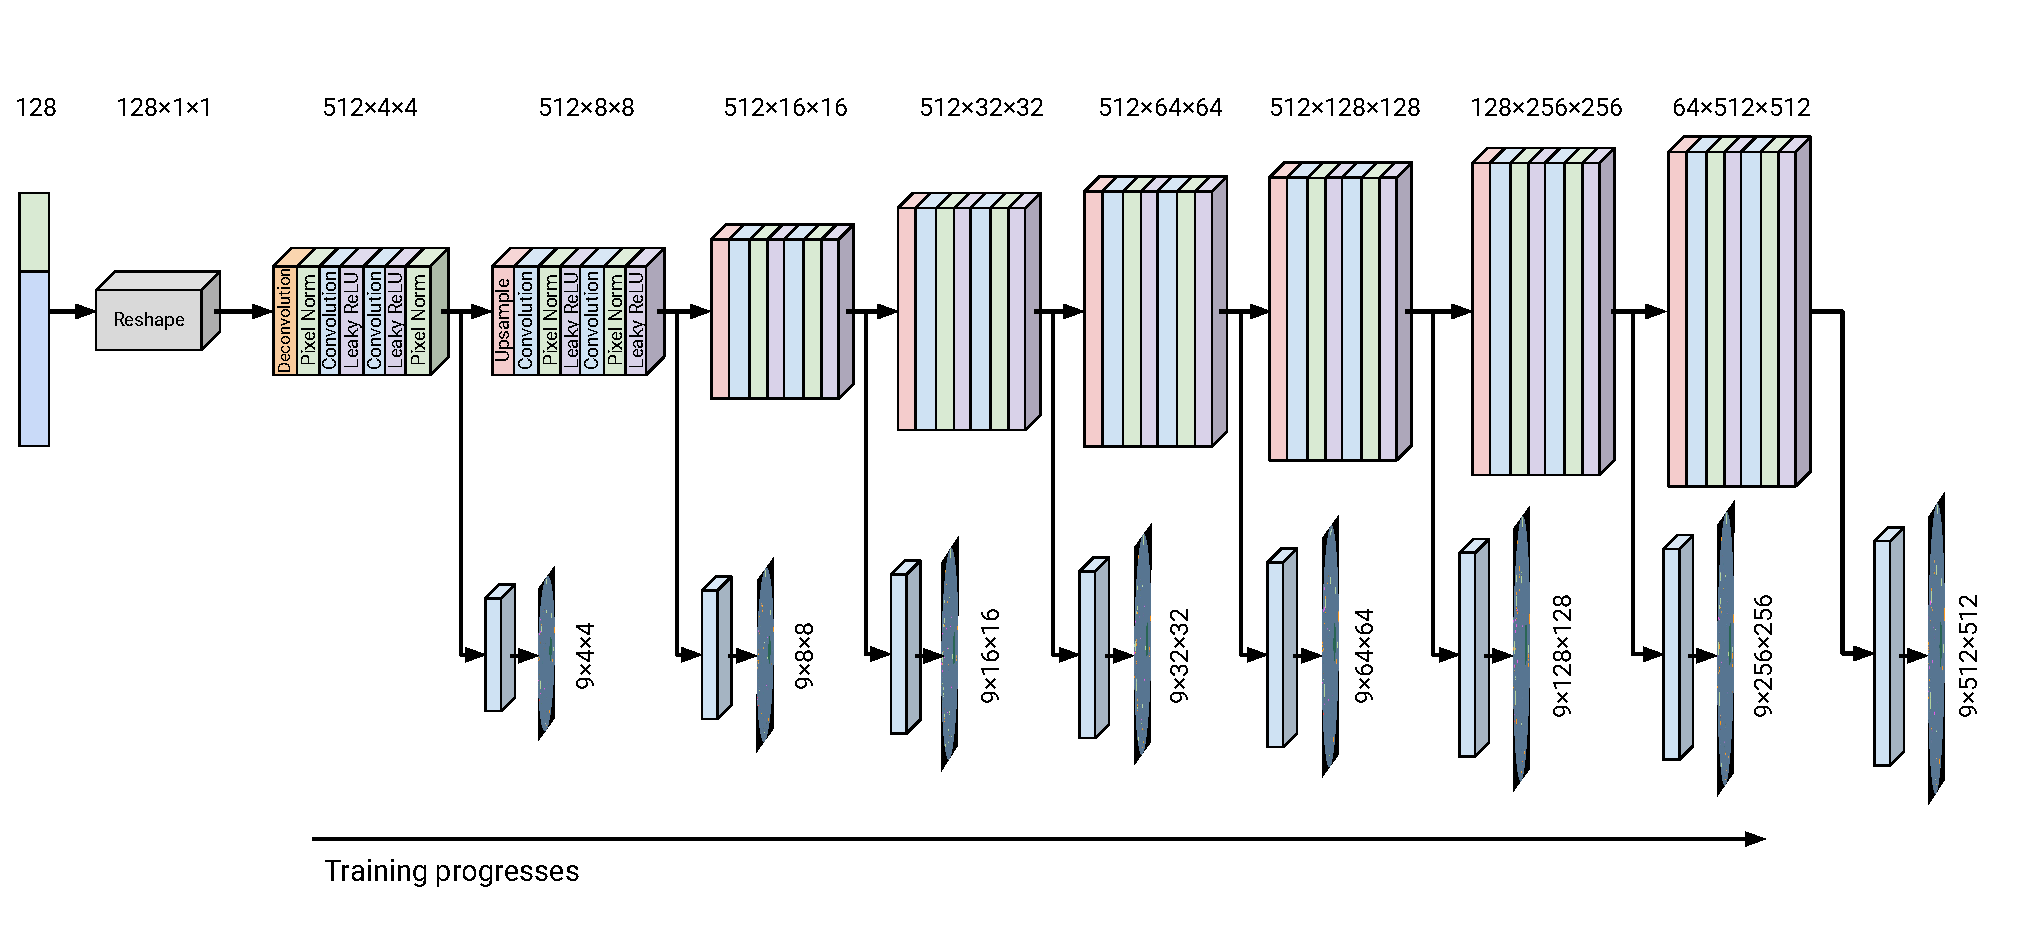
\includegraphics[width=\linewidth]{labels/figs/progan-generator.pdf}
        \caption{ProGAN generator architecture.}
        \label{fig:progan_gen}
    \end{subfigure}
    \begin{subfigure}{\textwidth}
        \centering
        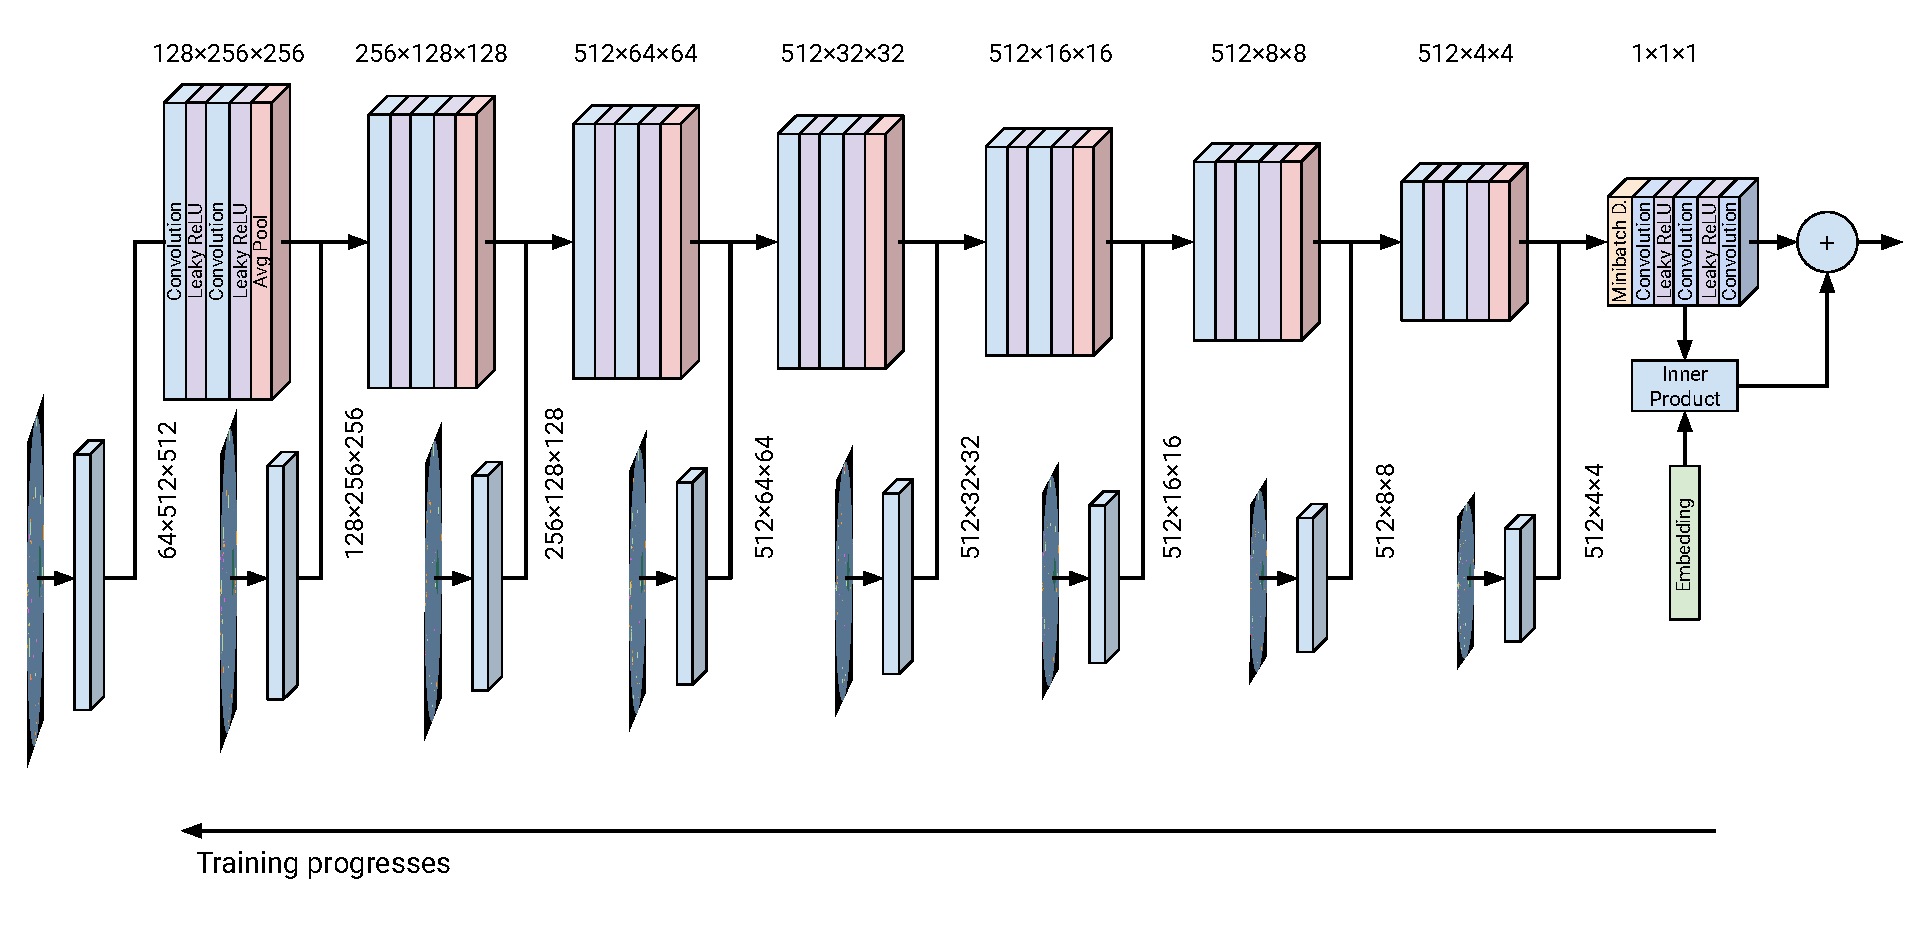
\includegraphics[width=\linewidth]{labels/figs/progan-discriminator.pdf}
        \caption{ProGAN discriminator architecture.}
        \label{fig:progan_dis}
    \end{subfigure}
    \caption{ProGAN network architectures.}
    \label{fig:progan_arch}
\end{figure}

As discussed, much of the instability we experienced when attempting to train semantic label generation GANs was owing to the discriminator's confidence, and the generator being unable to ``catch up''.
We also know that higher resolution images are more discriminable than lower resolution images.
Hence, it's intuitive that by starting at lower resolutions and progressively growing the generator and discriminator -- and therefore the resolution at which they operate -- the networks will be appropriately balanced throughout training.
Indeed, we found this to be the case, and that by allowing the generator to start with very small resolutions, the use of a ResNet-based discriminator was possible.
The generator and discriminator capacities are also very balanced, particularly in comparison to the ACGAN, with the generator having 24,639,137 parameters and the discriminator 24,646,209.


We use a ProGAN architecture to generate images starting from a resolution of $4\times 4$ up to $512\times 512$.
The generator and discriminator architectures are depicted in \Cref{fig:progan_arch}, with each additional block being capable of generating or discriminating images at a greater resolution.
In order to support variable sized images during training, we use \lstinline{toRGB} blocks in the generator, which are simply $1\times 1$ convolutions that reduce the number of feature maps down to the nine required in the output.
This allows us to create images at different resolutions while retaining the parameters learned in the prior hidden layers.
Conversely, \lstinline{fromRGB} blocks are used in the discriminator to increase the number of feature maps. 

We retain many of the same techniques detailed above, including label smoothing, the same loss function, and ADA.
However, we found that techniques that we relied upon with the fixed-resolution ACGAN, such as ADA, had a significantly weaker effect here.
We also incorporate some of the improvements detailed in the original ProGAN paper such as equalised learning rates and pixelwise feature vector normalisation in the generator \cite{DBLP:journals/corr/abs-1710-10196}.

To condition the generator, we simply concatenate the one-hot encoding of the class with the latent noise vector $z$.
We also experimented with using categorical batch normalisation as the conditioning strategy, but found that this caused mode collapse within each class.

\subsection{Optimiser}

We use the Adam optimiser with $\alpha_G = 0.0005$, $\alpha_D= 0.0001$, $\beta_1 = 0.0$, $\beta_2 = 0.99$ (same $\beta$ values as in the original ProGAN paper).
Unlike the ACGAN configuration, we perform just one generator training iteration for each discriminator training iteration.

\subsection{Equalised Learning Rate}

We use an equalised learning rate, where weights are initialised in the first instance using $\mathcal{N}(0, 1)$, and scaled dynamically during training.
Specifically, we set
\begin{align}
    \hat{w_i} = \frac{w_i}{c}
\end{align}
where $c$ is the per-layer normalisation constant from He initialisation \cite{he2015delving},
\begin{align}
    c = \sqrt{\frac{2}{n_l}}
\end{align}
and $n_l$ is the number of neurons in a layer.

\subsection{Pixelwise Feature Vector Normalisation}

We scale the feature vector of each pixel to unit length after each convolutional layer to prevent excessive signal magnitudes.
For the feature vector at pixel $(x, y)$, $a_{x, y}$, we obtain the normalised feature vector $b_{x, y}$ by
\begin{align}
        b_{x, y} = \frac{a_{x, y}}{\sqrt{\frac{1}{N} \sum_{j=0}^{N-1} a^i_{x, y} + \epsilon}}
\end{align}
where $N$ is the number of feature maps and $\epsilon = 10^{-8}$.

\subsection{Minibatch Standard Deviation}

In this technique, we first compute the standard deviation over each feature and spatial location in a minibatch.
We take the average of these standard deviations to yield a single value, which is then repeated and appended as an additional feature map.

\subsection{Projection Discriminator}

Introduced by \citeauthor{miyato2018cgans} \cite{miyato2018cgans}, in a projection discriminator, a projection between the feature maps and condition is added to the discriminator output.
This is computed as
\begin{align}
    f(x, y) = y^\intercal V \phi(x) + \psi (\phi(x))
\end{align}
where $x$ is the feature vector, $y$ is the class, and $V$ is the class embedding matrix -- making $y^\intercal V$ the corresponding embedding vector.
The transformations $\phi$ and $\psi$ are implemented as convolutional layers. 

\subsection{Training}

For each fade-in phase, we calculate the alpha value to merge images from the new and old resolution.
We spend 50\% of each phase fading in the previous resolution using a residual block to ``merge'' the new and old resolutions.
The length of each phase in the training regime is shown in \Cref{tab:progan_training}.

\begin{table}[h]
    \centering
    \begin{tabular}{lccccccccc}
        \toprule
        Resolution & $4^2$ & $8^2$ & $16^2$ & $32^2$ & $64^2$& $128^2$& $256^2$& $512^2$ \\
        \midrule
        Epochs & 20 & 40 & 60 & 80 & 100 & 120 & 140 & 160 \\
        Batch size & 512 & 256 & 128 & 64 & 32 & 16 & 8 & 4 \\
        \bottomrule
    \end{tabular}
    \caption{ProGAN training phases.}
    \label{tab:progan_training}
\end{table}

% \begin{figure}[h]
%     \centering
%     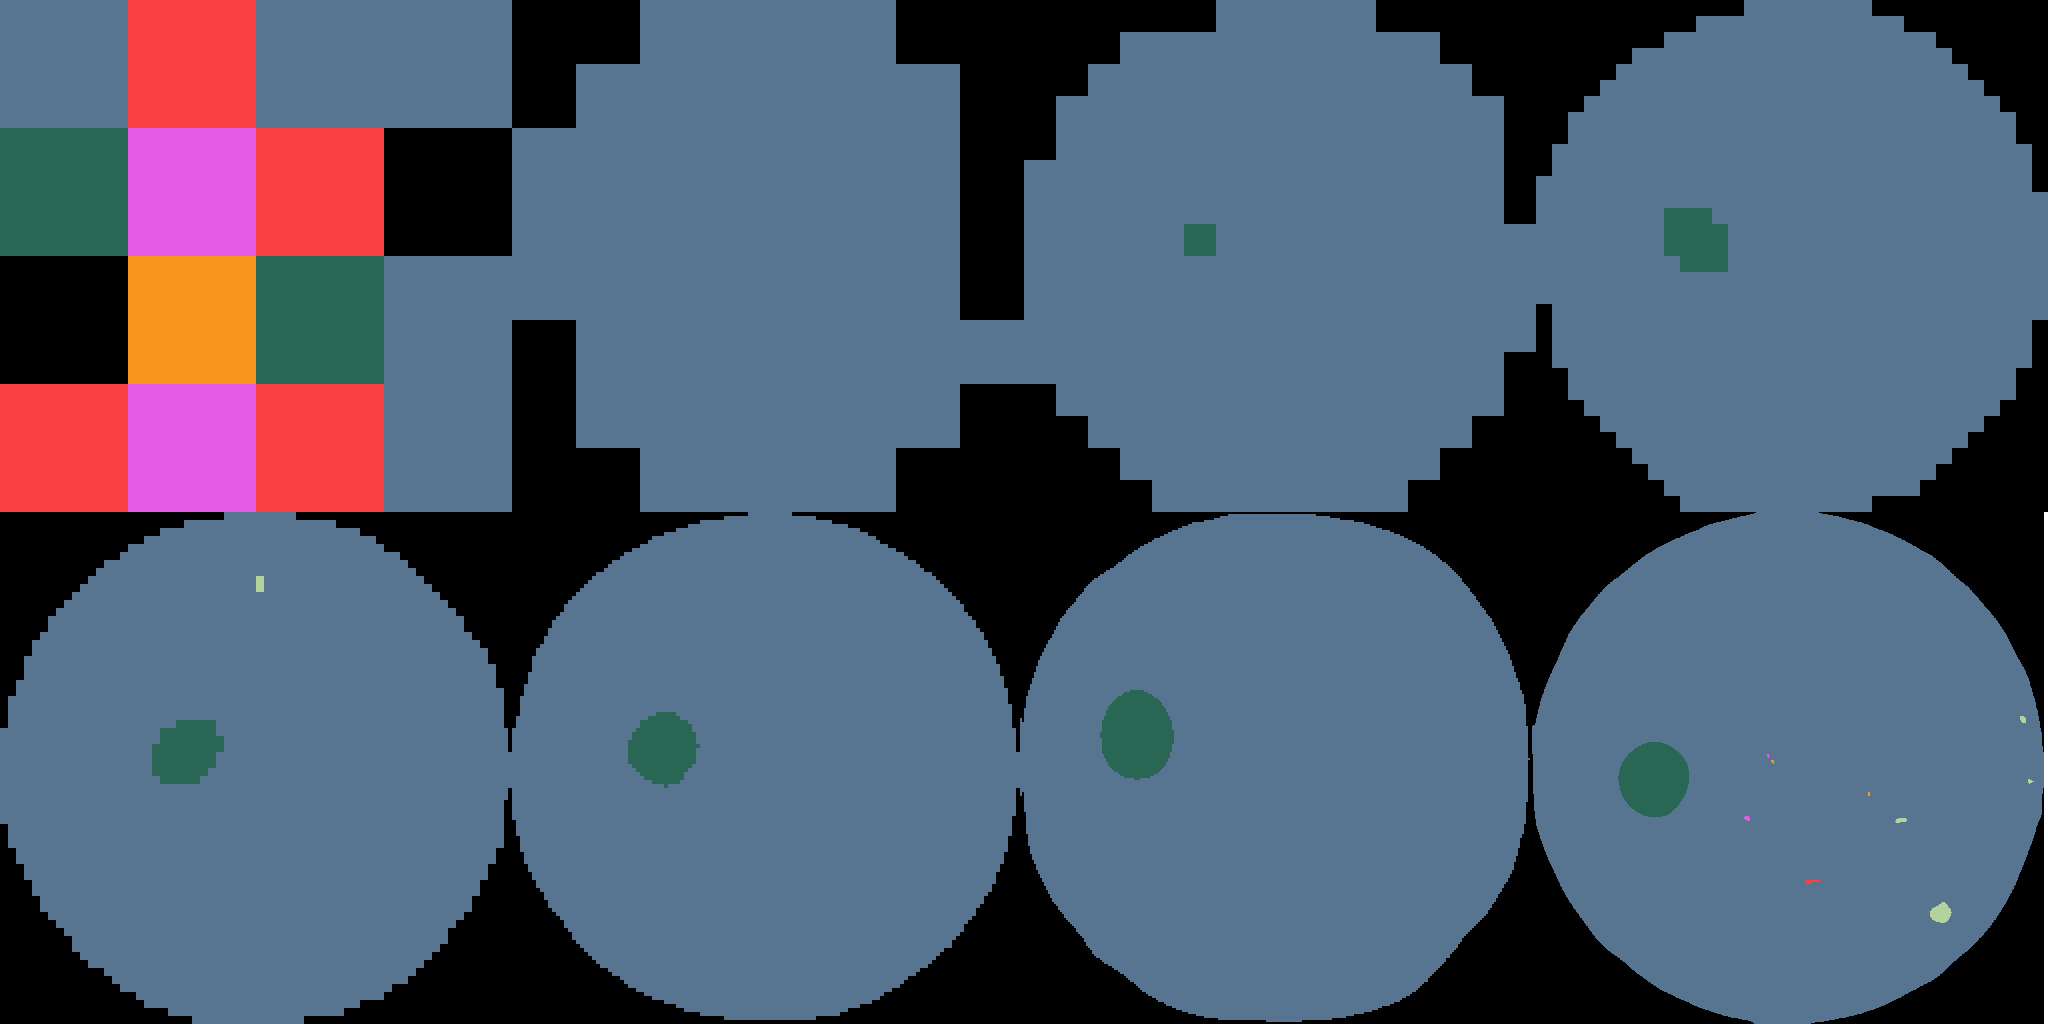
\includegraphics[width=0.5\textwidth]{labels/figs/progressive-growing.png}
%     \caption{Samples taken during training at resolutions from $4\times 4$ to $512 \times 512$.}
%     \label{fig:progressive_grow}
% \end{figure}
% 
%  as shown in \Cref{fig:progressive_grow}.

\section{Copy-Paste}

\begin{figure}[h]
    \centering
    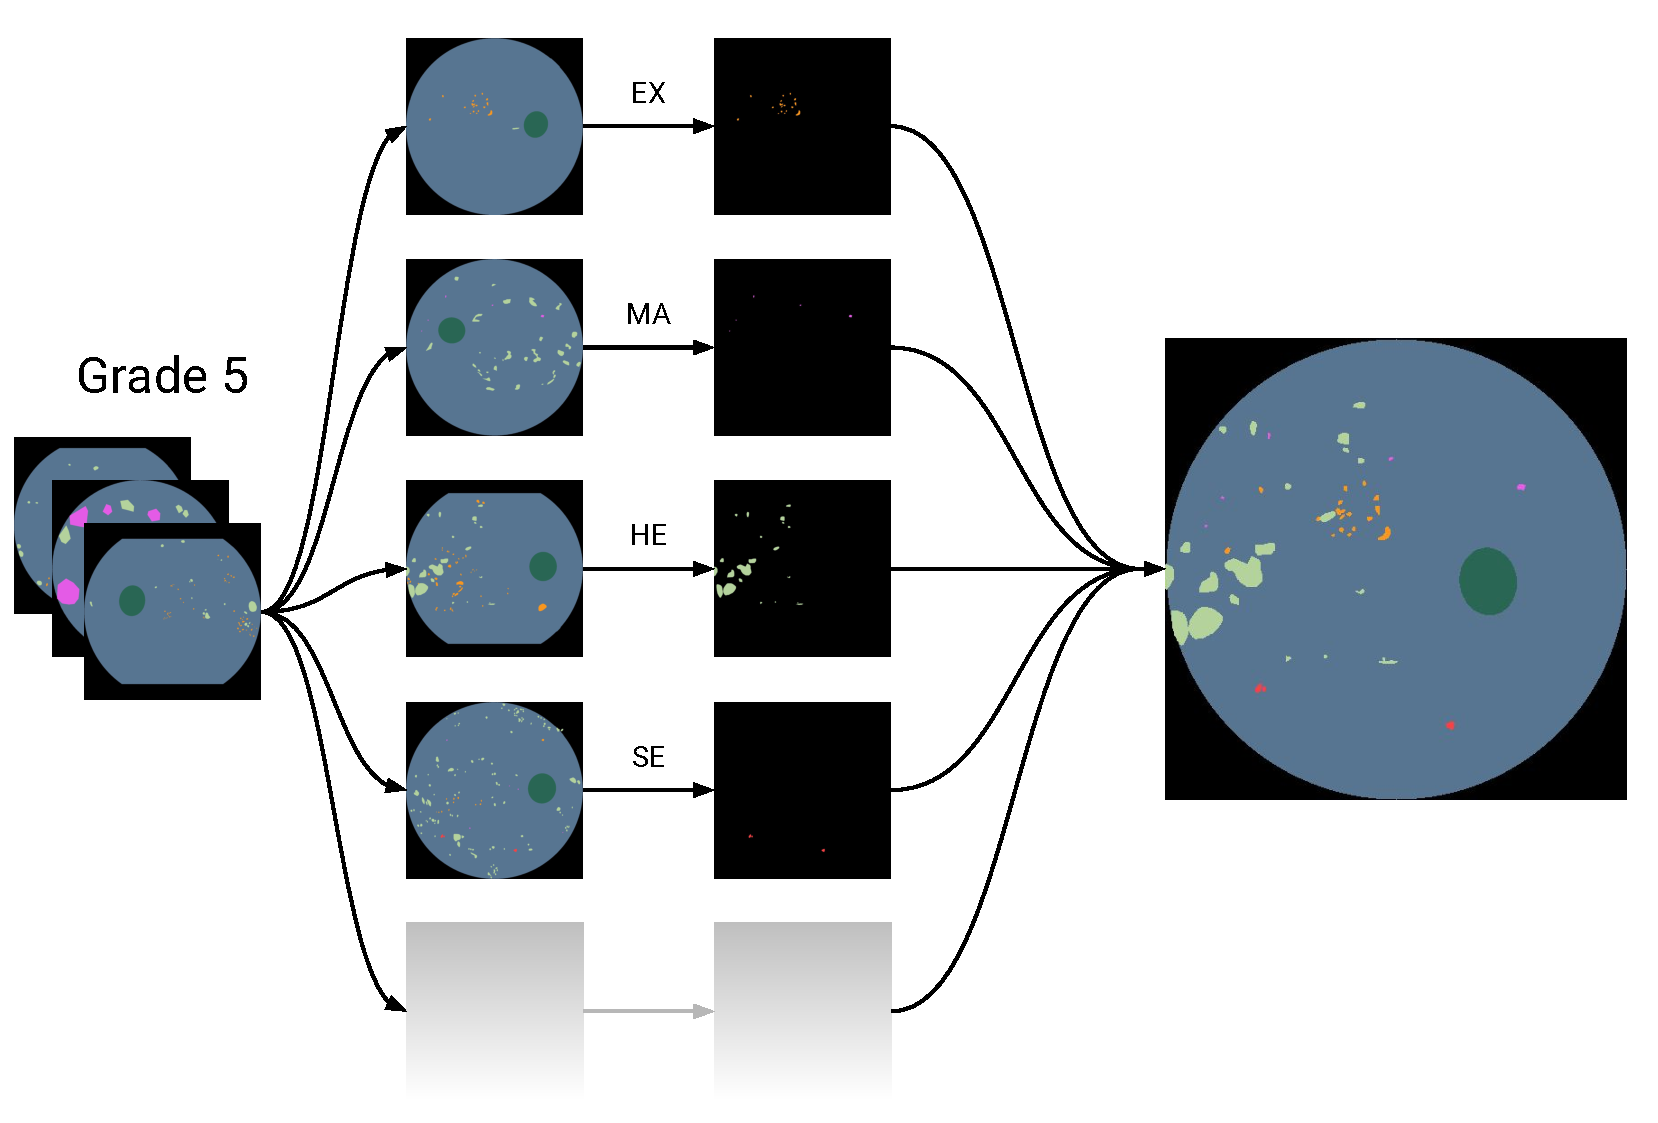
\includegraphics[width=0.6\textwidth]{labels/figs/copy-paste}
    \caption{Illustration of copy-paste generation.}
    \label{fig:copypaste}
\end{figure}

\citeauthor{ghiasi2020simple} \cite{ghiasi2020simple} showed that simply copy-and-pasting objects onto a scene can improve the performance of instance segmentation algorithms on natural images.
Inspired by this, we introduce a simple and efficient data augmentation technique that uses multi-label sampling to generate new data for semantic segmentation.
We refer to this technique as ``copy-paste''.
To generate copy-pasted data, semantics labels for each class are randomly sampled from existing data and concatenated in order to create a new semantic label of the same grade.
This process is depicted in \Cref{fig:copypaste}.

The advantages of this method are clear in that it requires very few compute resources and no prior training, while still being able to create a diverse range of samples.
It is only possible because the layout of each image is uniform, and we are not limited by rigid structures such as vessels (which are filled in by the image-to-image translation network).
In this sense, retinal fundus images are a very flexible target modality -- the same method would be difficult to apply on, for example, the Cityscapes dataset.

Of course, this approach does not take into account any knowledge \emph{a posteriori} about the retinal structure or relationship between lesions.
Hence, images generated using this method can exhibit overlapping, or implausible semantic labels.
Nevertheless, these same issues can arise with GANs; it may even be the case that certain lesions are simply too difficult or too small for the GANs (in their current form) to generate, whereas copy-paste has no such limitations.

As before, we take care to prevent data leakage by sampling new data points from only the fixed training set.
We could also apply scale and position jittering to further increase diversity, but we leave this as a future investigation.

\section{Experiments}

For all ACGAN experiments, we set the batch size to 64 and trained for 2000 epochs.
Early experiments included ``slow'' (e.g. 100 generator, 100 discriminator iterations per batch) and ``fast'' (e.g. 1 generator, 1 discriminator iteration per batch) training schemes, and exploring different variants on ADA, such as annealing the maximum $p$ value over time, or tweaking the types of transformation.
Rather predictably, any change that increased the probability of discriminator overfitting was likely to cause training to collapse.
We also test a variant of the ACGAN where we condition the generator by concatenating the embedded class vector with the latent dimension, instead of taking the Hadamard product.

\begin{figure}[h]
    \centering
    \begin{subfigure}{0.45\textwidth}
        \centering
        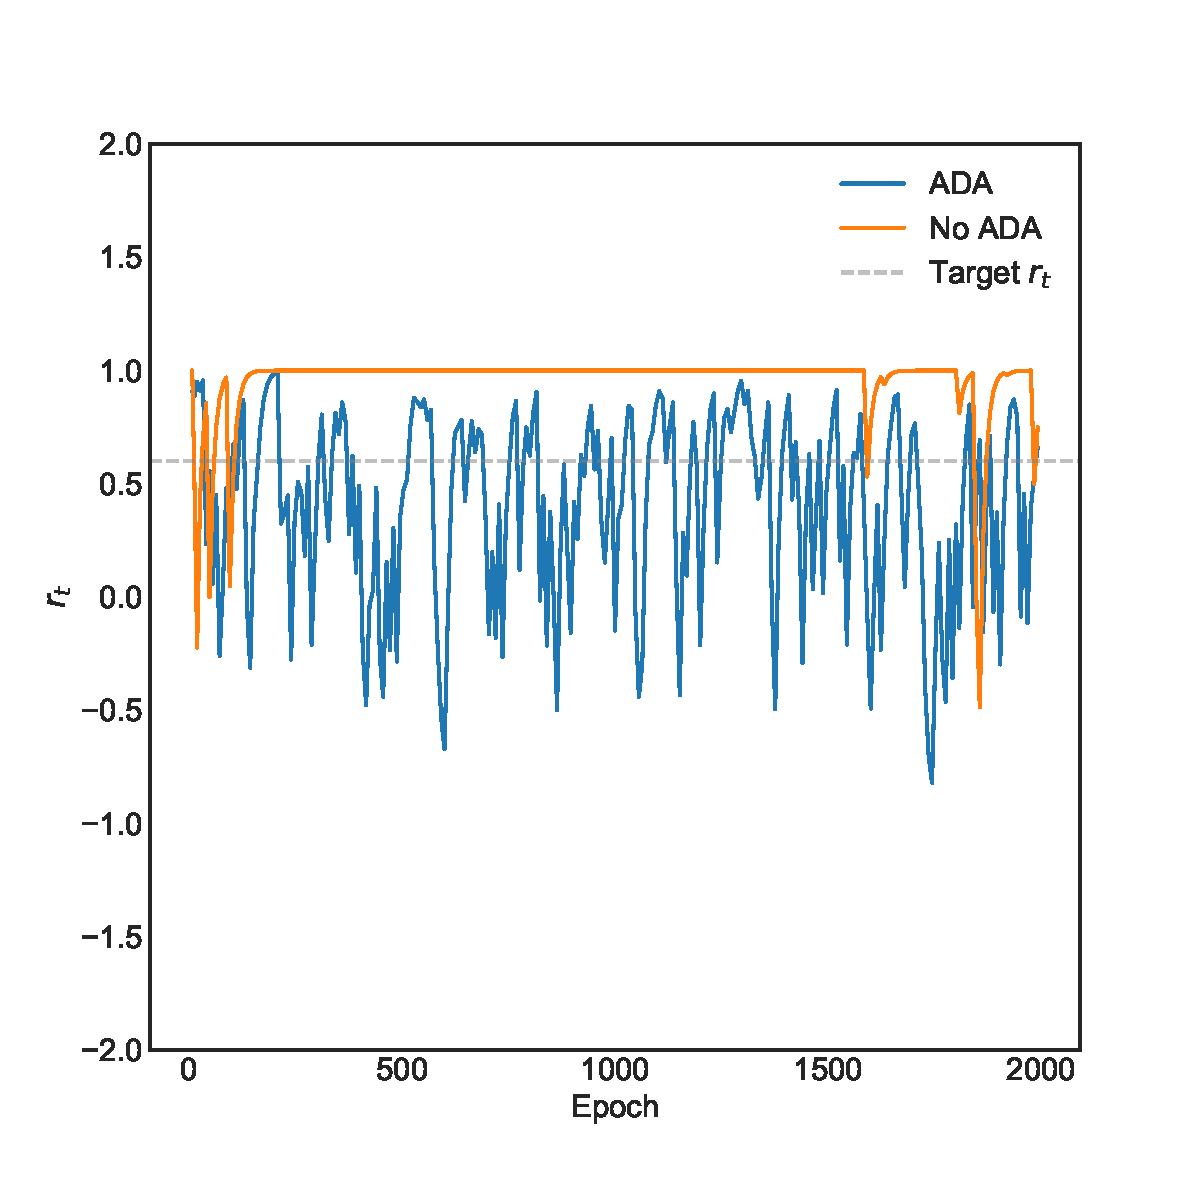
\includegraphics[width=\linewidth]{labels/figs/ada_r_t.pdf}
        \caption{Value of $r_t$ during training.}
        \label{fig:acgan_ada_r_t}
    \end{subfigure} %
    \begin{subfigure}{0.45\textwidth}
        \centering
        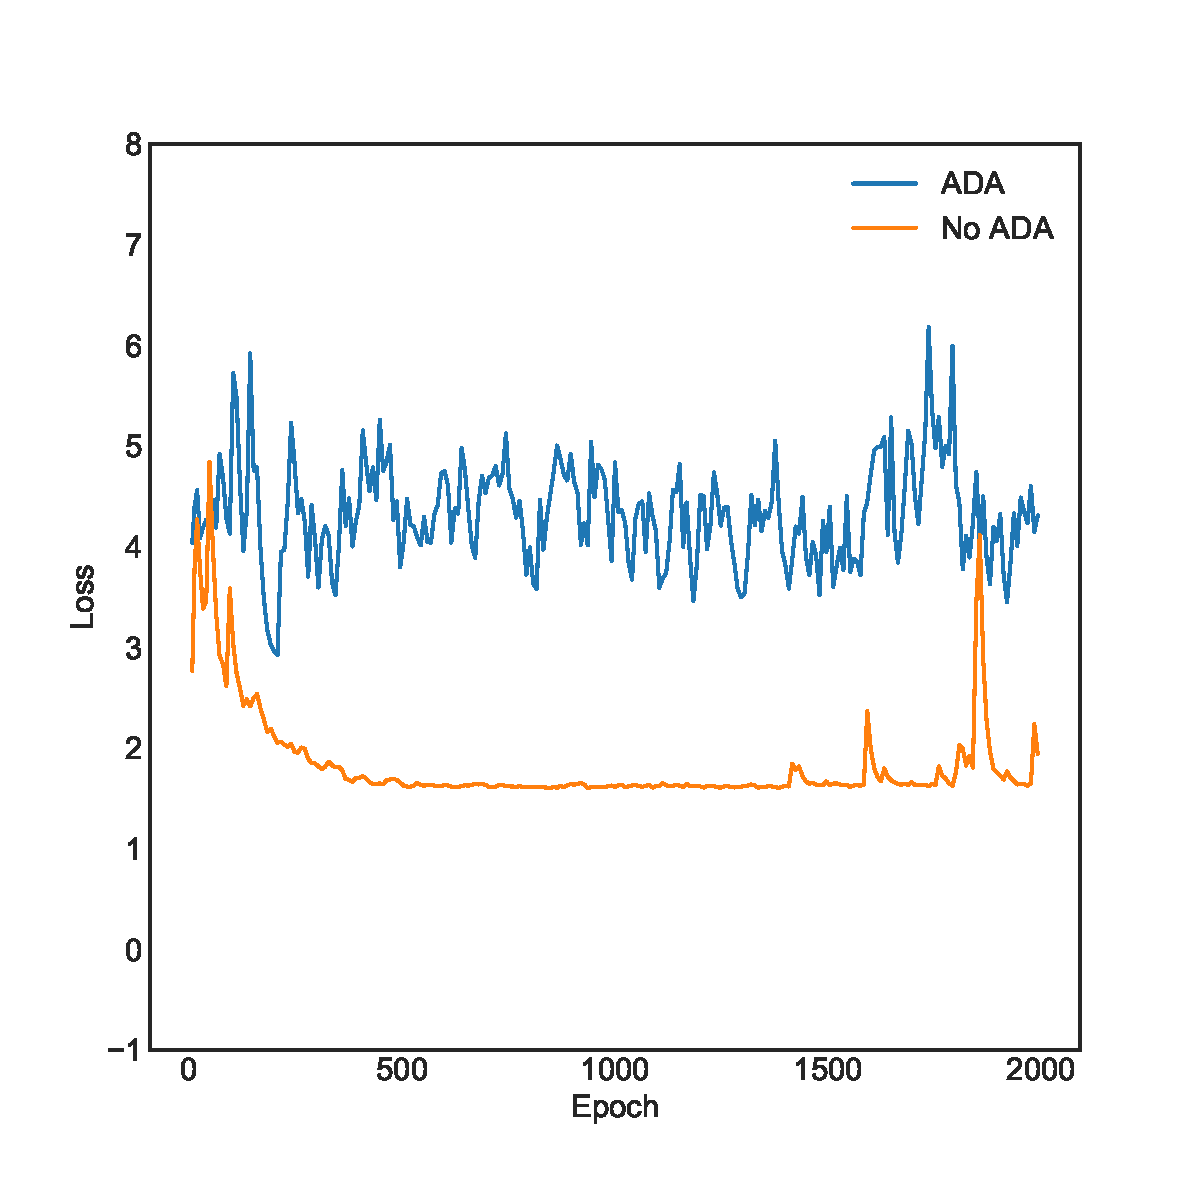
\includegraphics[width=\linewidth]{labels/figs/ada_dis.pdf}
        \caption{Discriminator loss during training.}
        \label{fig:acgan_ada_dis}
    \end{subfigure}
    \caption{Comparison between training with and without ADA.}
    \label{fig:acgan_ada}
\end{figure}

To investigate the importance of ADA to GAN stability, we trained the ACGAN with and without ADA and compared how training developed over time.
From \Cref{fig:acgan_ada}, we can see that without ADA the adversarial discriminator loss quickly collapses.
Note that the total discriminator loss does not go to zero due to the magnitude of the auxiliary losses.
The overfitting heuristic $r_t$ immediately rises to its maximum possible value of 1, and remains there for essentially the rest of training.
The generator is unable to recover from this.
Conversely, when we apply ADA, we are able to use the negative feedback from $r_t$ to increase the probability of augmentations to reduce discriminator overfitting, and thereby keep training relatively stable.

The processing and memory usage required by the ProGAN is significantly higher, which caused batch sizes to be smaller, and overall training times to be much longer.
As a result, we used a batch size of 8 for the ProGAN.
A side-effect of this was that $r_t$ and $p$, which are updated every batch, were much noisier during training for the ProGAN than the ACGAN.

\subsection{Samples}

\begin{figure}[h]
    \centering
    \begin{subfigure}{0.31\textwidth}
        \centering
        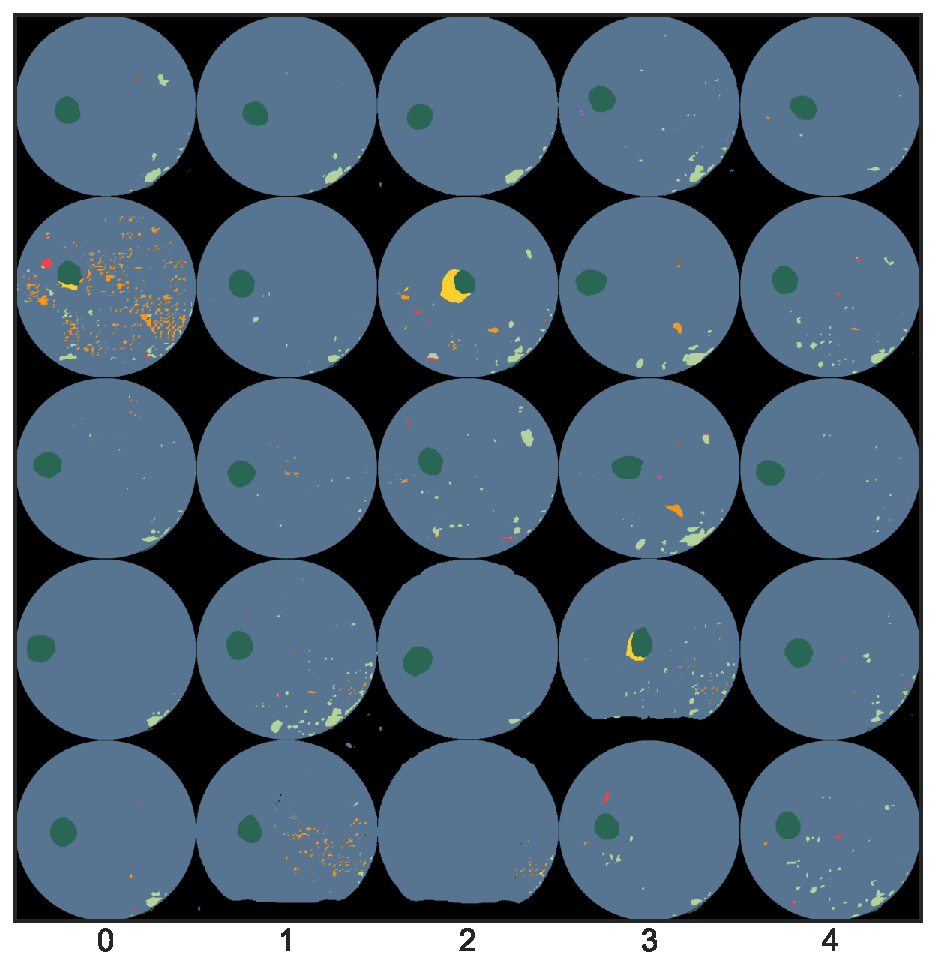
\includegraphics[width=\linewidth]{labels/figs/acgan_sample.pdf}
        \caption{ACGAN}
        \label{fig:acgan_sample}
    \end{subfigure}
    \begin{subfigure}{0.31\textwidth}
        \centering
        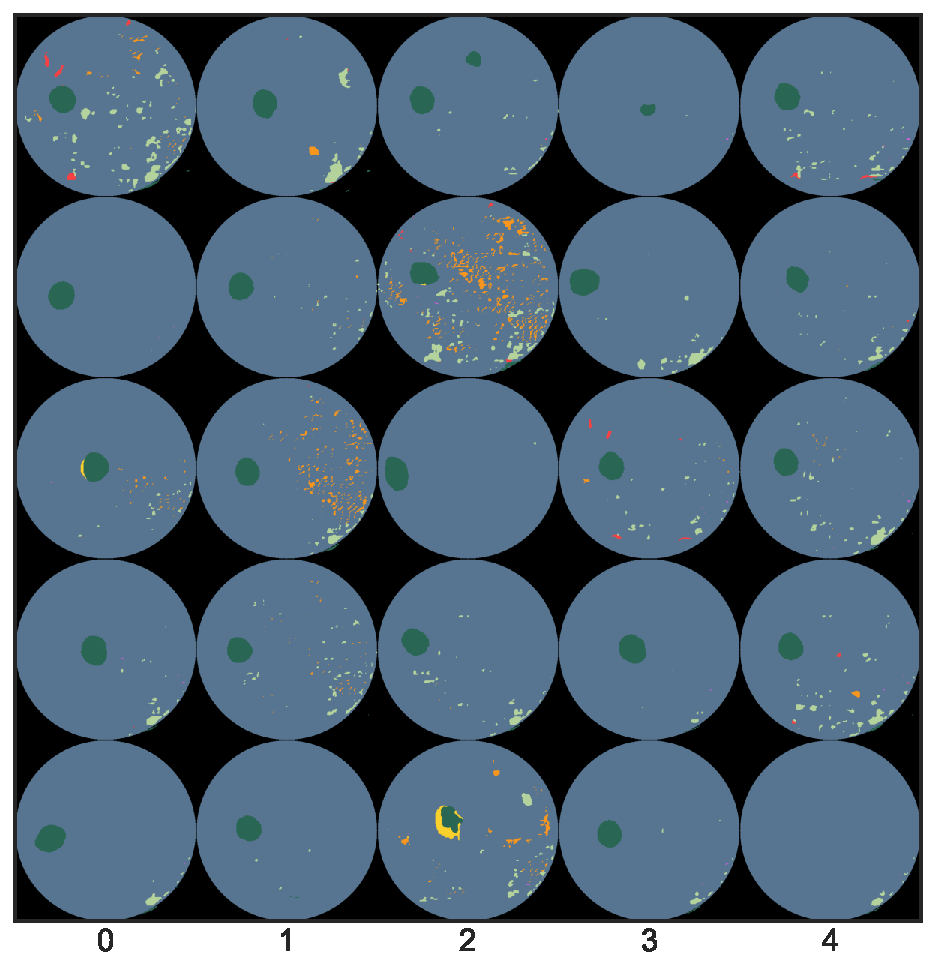
\includegraphics[width=\linewidth]{labels/figs/acgan_mask_sample.pdf}
        \caption{ACGAN + mask}
        \label{fig:acgan_sample_2}
    \end{subfigure}
    \begin{subfigure}{0.31\textwidth}
        \centering
        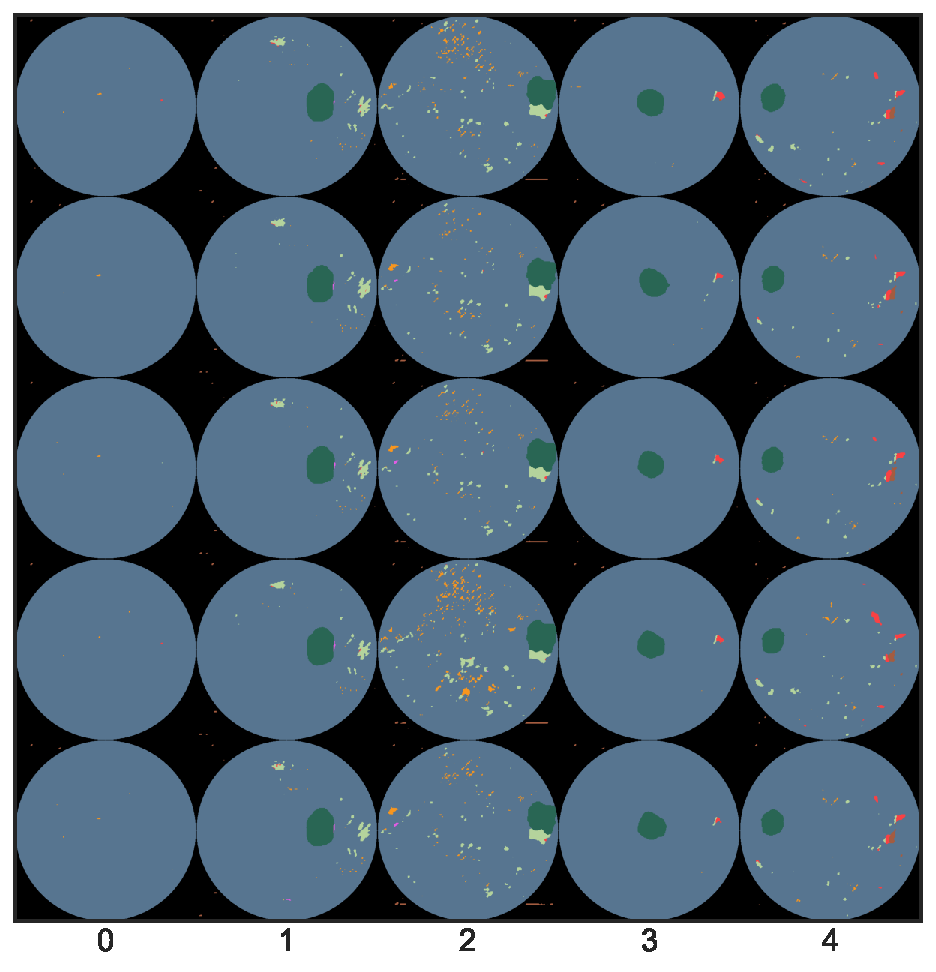
\includegraphics[width=\linewidth]{labels/figs/acgan_concat_sample.pdf}
        \caption{ACGAN + mask, concat.}
        \label{fig:acgan_sample_3}
    \end{subfigure}
    \begin{subfigure}{0.31\textwidth}
        \centering
        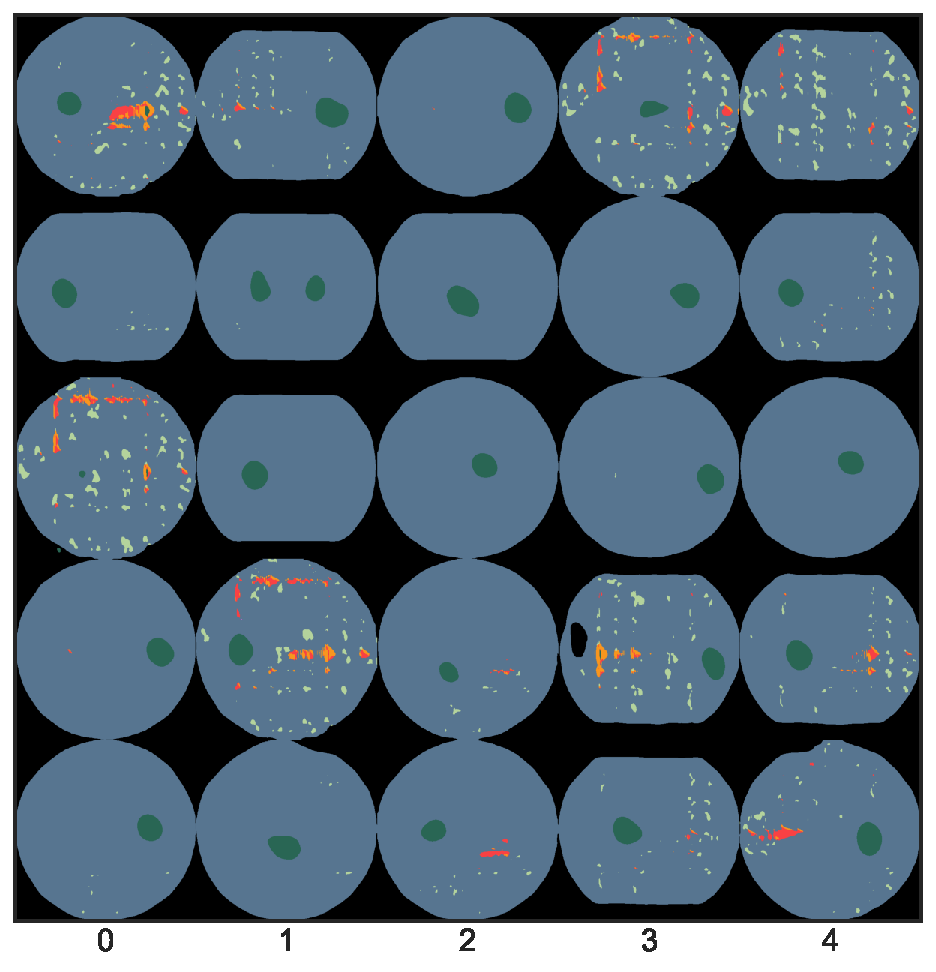
\includegraphics[width=\linewidth]{labels/figs/progan_sample.pdf}
        \caption{ProGAN}
        \label{fig:progan_sample}
    \end{subfigure}
    \begin{subfigure}{0.31\textwidth}
        \centering
        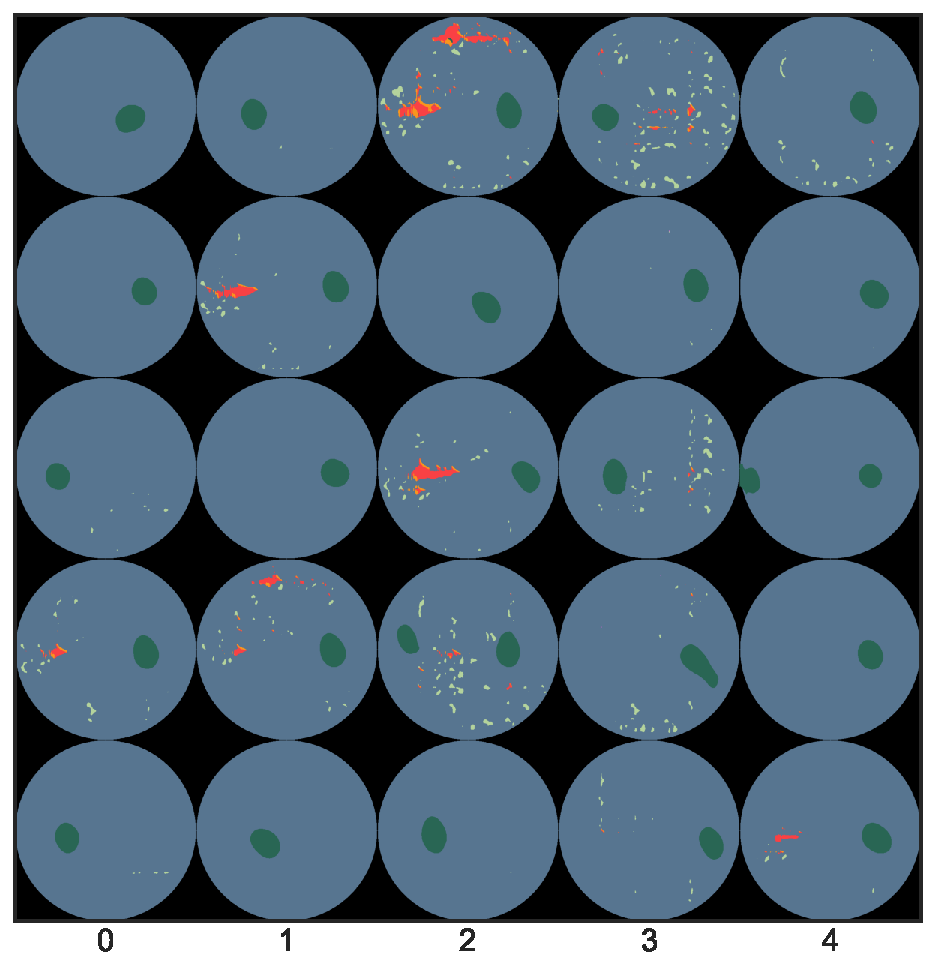
\includegraphics[width=\linewidth]{labels/figs/progan_mask_sample.pdf}
        \caption{ProGAN + mask}
        \label{fig:progan_sample_2}
    \end{subfigure}
    \begin{subfigure}{0.31\textwidth}
        \centering
        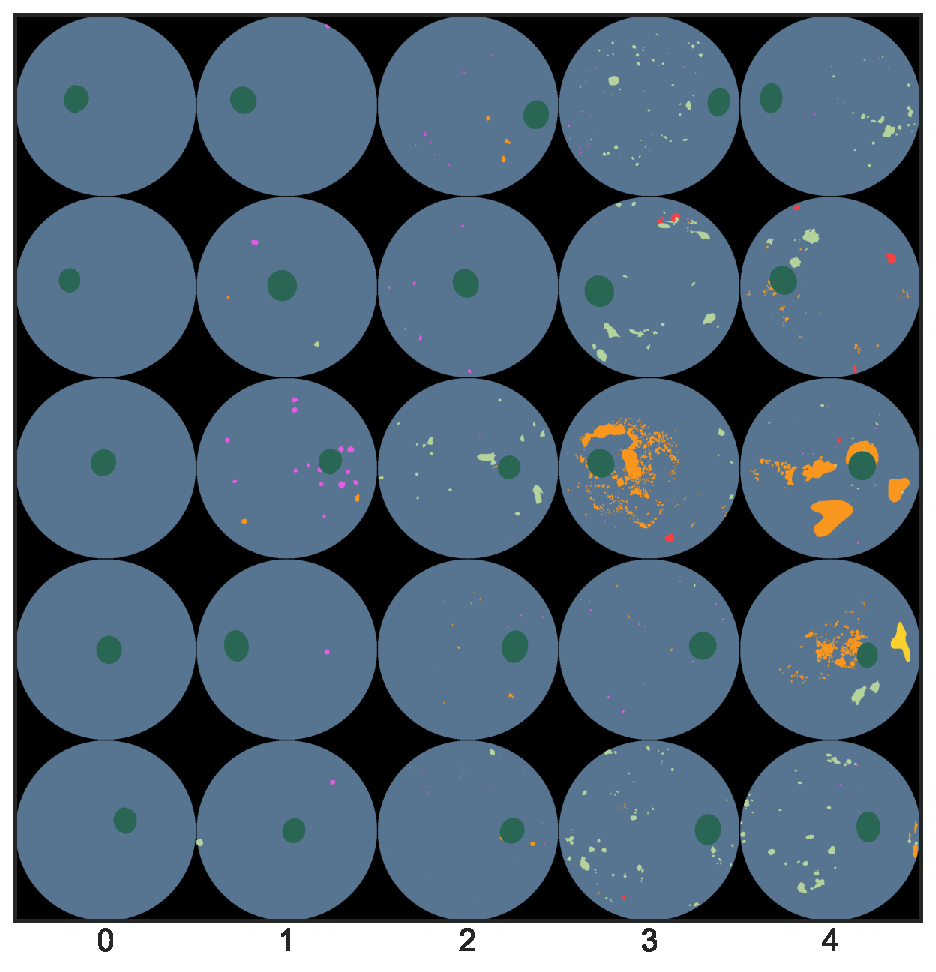
\includegraphics[width=\linewidth]{labels/figs/copypaste_sample.pdf}
        \caption{Copy-Paste}
        \label{fig:copypaste_sample}
    \end{subfigure}
    \caption{Sample of generated semantic labels for each configuration. Columns from left to right correspond to input DR grades 0 through 4.}
    \label{fig:semantic_label_sample}
\end{figure}

A sample of generated images is shown in \Cref{fig:semantic_label_sample}.
From a brief visual examination, the GANs appear have successfully been able to capture the form of the semantic labels.
The conditioning, however, has been less successful.
Only the ACGAN with concatenation has been able to learn a definite conditioning, but it suffers mode collapse within each of the classes.
We can also see a number of recurring modes in the ACGAN and ProGAN samples, which is indicative of low diversity.
Meanwhile, the copy-pasted data shows a diverse range of samples, and is clearly well-conditioned. 
Despite this, there are some instances where the optic disc has been pasted directly on top lesions, which is unrealistic.
The ``mask'' variants have an additional post-processing step applied in which the fundus boundary is masked as a circle.
This is in response to a failure mode discussed in the next section.

\subsection{Common Failure Modes}

\begin{figure}[h]
    \centering
    \begin{subfigure}[t]{0.19\textwidth}
        \centering
        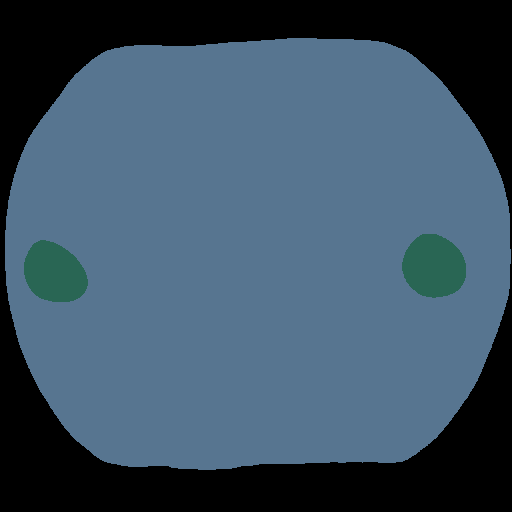
\includegraphics[width=\linewidth]{labels/figs/two-od.png}
        \caption{Multiple optic discs.}
        \label{fig:two_od}
    \end{subfigure} %
    \hfill
    \begin{subfigure}[t]{0.19\textwidth}
        \centering
        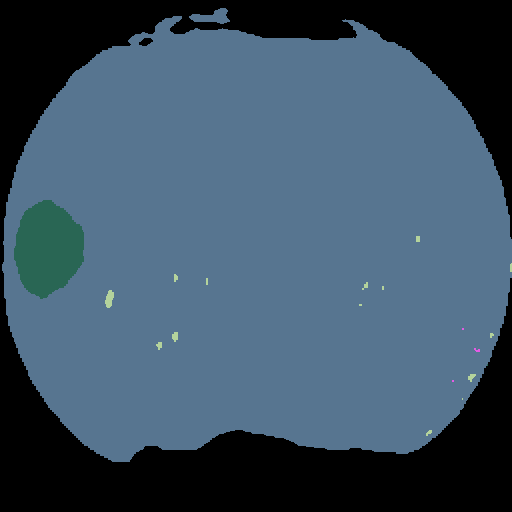
\includegraphics[width=\linewidth]{labels/figs/malformed-fundus.png}
        \caption{Malformed fundus.}
        \label{fig:malformed_fundus}
    \end{subfigure} %
    \hfill
    \begin{subfigure}[t]{0.19\textwidth}
        \centering
        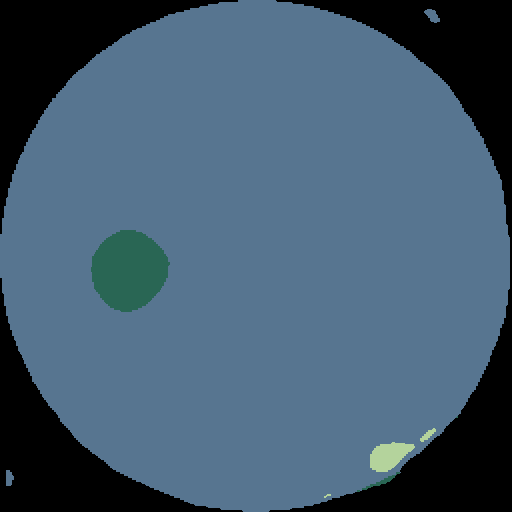
\includegraphics[width=\linewidth]{labels/figs/spurious-pixels.png}
        \caption{Spurious pixels.}
        \label{fig:spurious_pixels}
    \end{subfigure} %
    \hfill
    \begin{subfigure}[t]{0.19\textwidth}
        \centering
        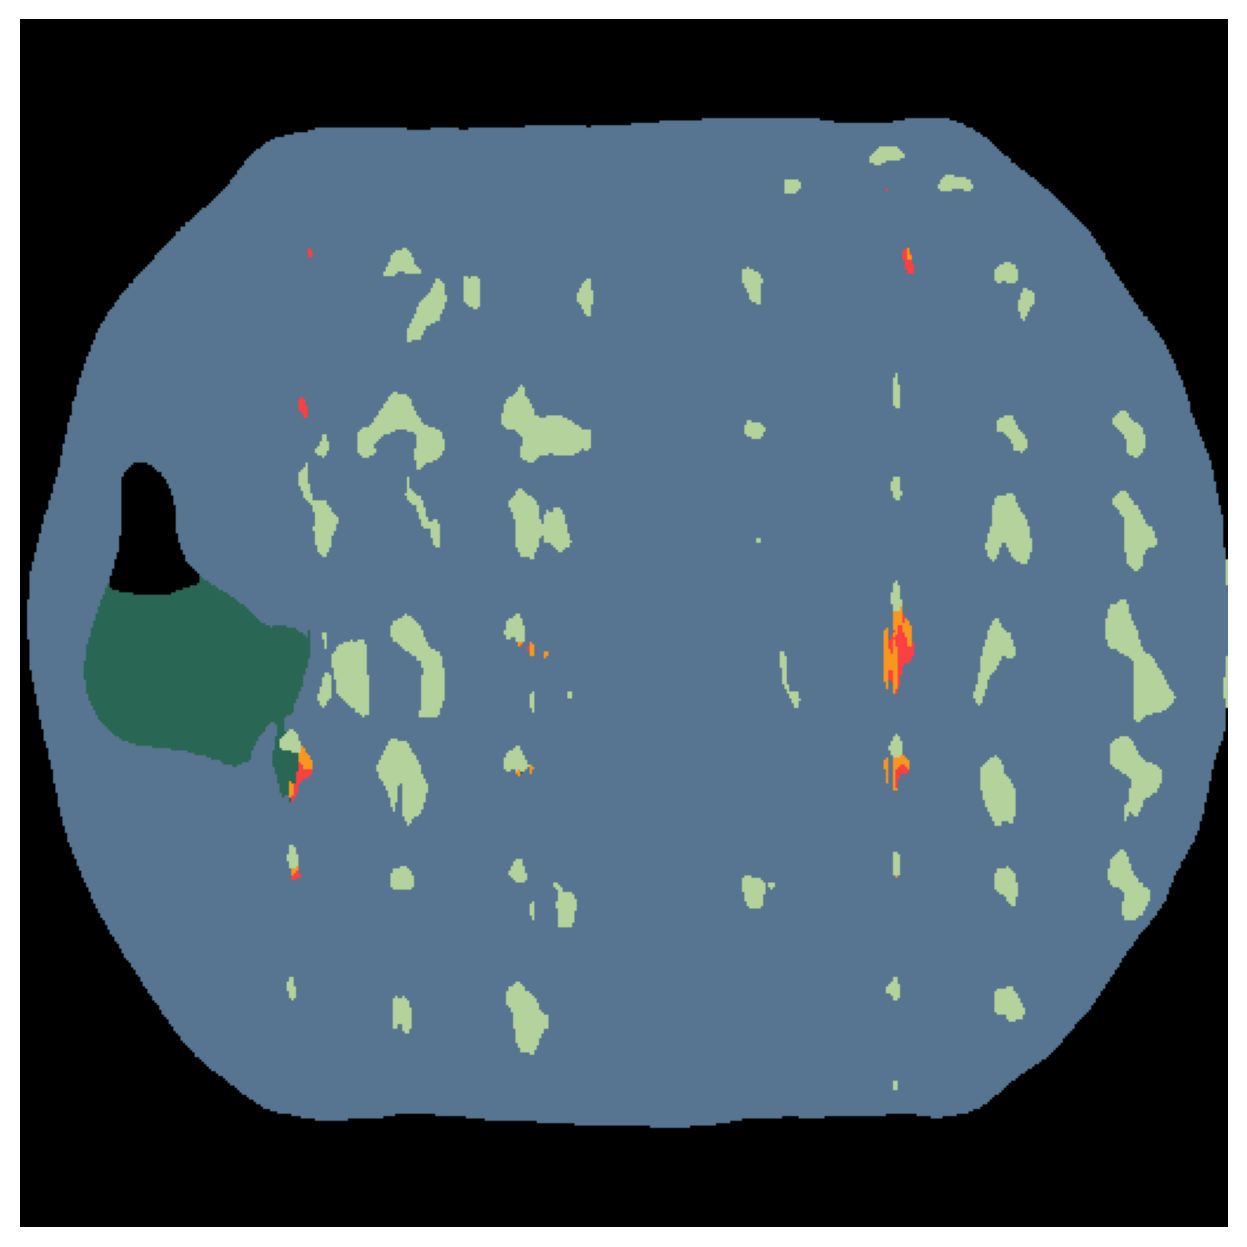
\includegraphics[width=\linewidth]{labels/figs/hole.png}
        \caption{Holes.}
        \label{fig:holes}
    \end{subfigure} %
    \hfill
    \begin{subfigure}[t]{0.19\textwidth}
        \centering
        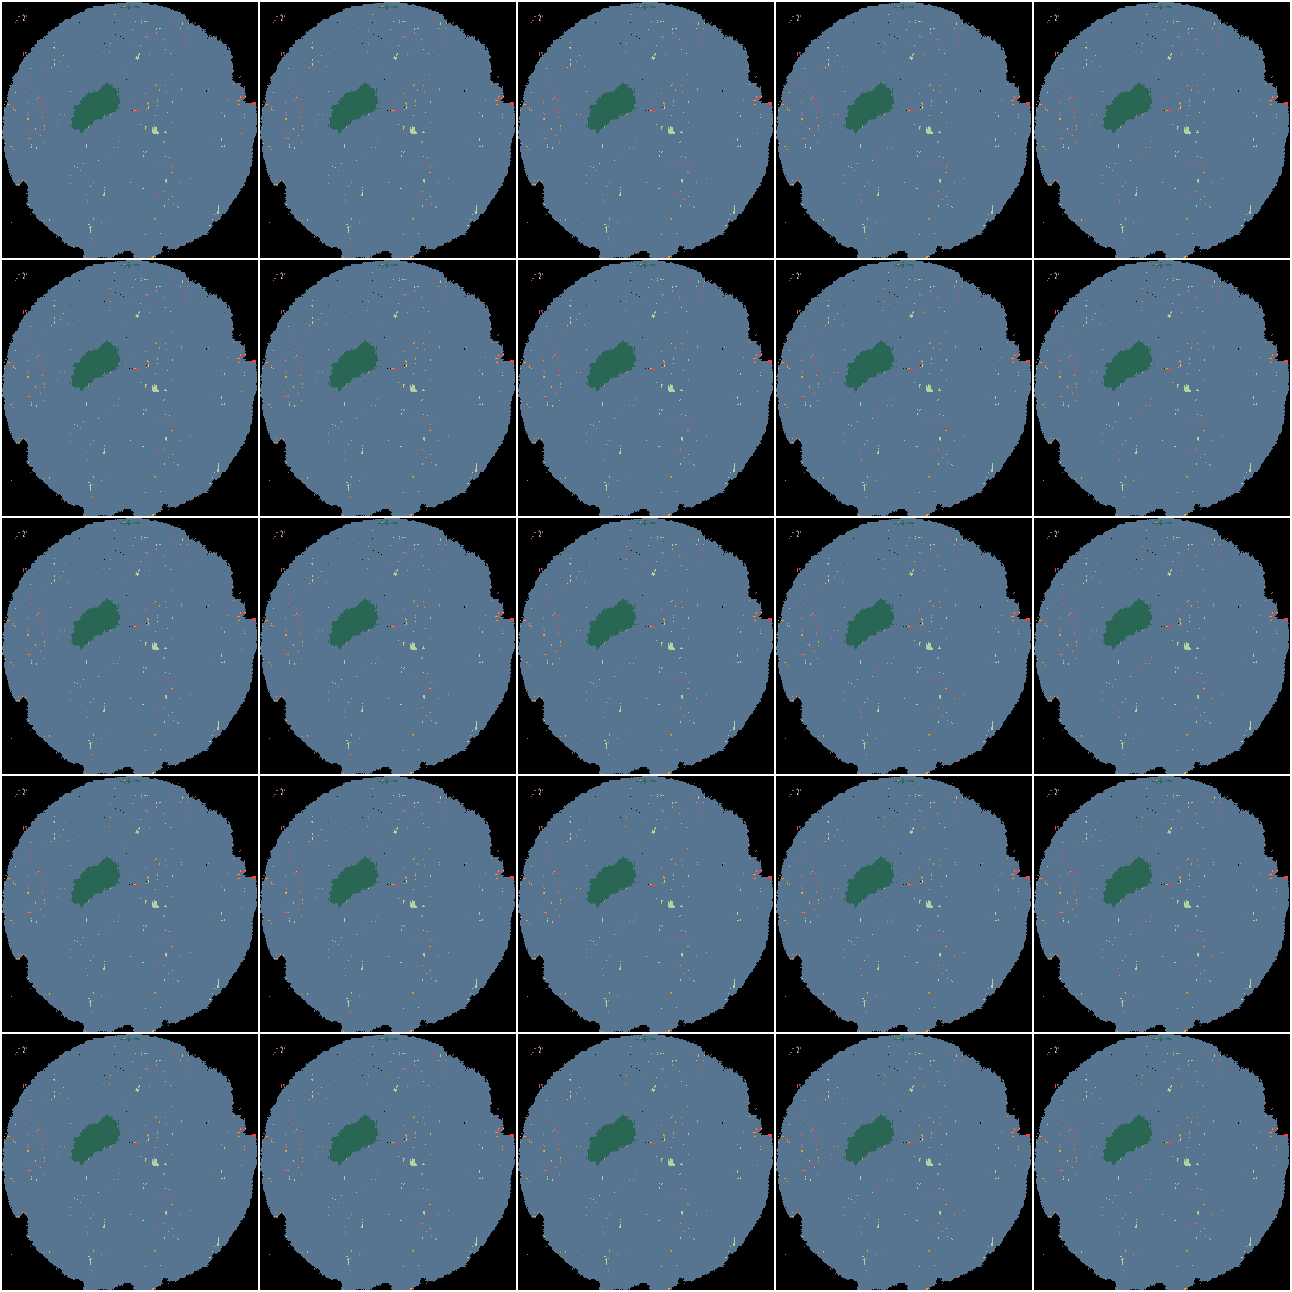
\includegraphics[width=\linewidth]{labels/figs/mode-collapse.png}
        \caption{Mode collapse.}
        \label{fig:mode_collapse}
    \end{subfigure} %
    \caption{Examples of common failure modes.}
    \label{fig:acgan_bad_sample}
\end{figure}

The models still display a number of failure modes which are yet to be addressed in the current iteration of this work.

\begin{description}
    \item[Multiple Optic Discs] \hfill \\ 
    There is a tendency to generate multiple optic discs, which is not possible in the source data. 
    Example shown in \Cref{fig:two_od}.
    
    \item[Malformed Fundus] \hfill \\ 
    Both GAN types encountered difficulty with generating geometric shapes, such as the circular fundus mask.
    One mitigation is to remove this responsibility from the generator and simply mask out the fundus as a post-processing step.
    Example shown in \Cref{fig:malformed_fundus}.
    
    \item[Spurious Pixels] \hfill \\ 
    If the GAN is over-trained, there is a point at which spurious pixels outside of the fundus boundary are generated.
    These kinds of artefacts are obviously unrealistic and not desirable.
    Example shown in \Cref{fig:spurious_pixels}.
    
    \item[Holes] \hfill \\ 
    Some images exhibit ``tears'' or gaps in the semantic labels. This is particularly prevalent with the ProGAN. 
    Example shown in \Cref{fig:holes}.
    
    \item[Low Diversity/Mode Collapse] \hfill \\ 
    As mentioned, the GANs can exhibit low diversity, even if this does not quite extend to total mode collapse.
    For instance, one can see from the ACGAN samples that the optic disc is generated in approximately the same spot in almost all samples.
    Without diversity, downstream models will be prone to overfitting to the synthetic data, decreasing performance. 
    This happens when the discriminator is too strong, which implies that we may need to inhibit the discriminator even further.
    Example shown in \Cref{fig:mode_collapse}.
\end{description}

\subsection{Results}

\begin{table}[h]
    \centering
    \begin{tabular}{lrrrrrr}
    \toprule
        Configuration & FID$\downarrow$ & Accuracy$\uparrow$ & Precision$\uparrow$ & Recall$\uparrow$ & $F_1$$\uparrow$ & $\kappa$$\uparrow$ \\
    \midrule
        Validation & 17.118 & 0.709 & 0.700 & 0.741 & 0.710 & 0.739 \\
    \midrule
        ACGAN & 64.388 & 0.191 & 0.249 & 0.187 & 0.115 & -0.004 \\
        + mask & 44.674 & 0.195 & 0.194 & 0.195 & 0.154 & 0.001 \\
        + mask, concatenation & 80.743 & 0.037 & 0.216 & 0.036 & 0.027 & 0.051 \\
    \midrule
        ProGAN & 51.970 & 0.206 & 0.194 & 0.205 & 0.142 & 0.020 \\
        + mask & 46.044 & 0.200 & 0.189 & 0.199 & 0.176 & 0.018 \\
    \midrule
        Copy-Paste & \textbf{21.717} & \textbf{0.691} & \textbf{0.688} & \textbf{0.691} & \textbf{0.686} & \textbf{0.807} \\
    \bottomrule
    \end{tabular}
    \caption{Metrics assessing the image and conditioning quality for each generation method. Best results for each metric in bold (excluding the baseline).}
    \label{tab:acgan_results}
\end{table}

To evaluate image quality, we compute the FID score between the coloured semantic labels of the training set and those of the target dataset.
Even though the FID is designed for natural looking images (after all, the Inception network is trained on Image-Net), and the semantic image colours are chosen arbitrarily, it seems to function as a fairly good proxy for visual quality and diversity regardless.
To evaluate the strength of DR grade conditioning, we trained a ResNet-50 network for 100 epochs on the 9-channel semantic labels of the FGADR subset of the real training data (since only these have annotations for DR severity labels).
We use this network to perform inference on generated data, and retrieve the accuracy, precision, recall, $F_1$, and $\kappa$ achieved.
This model was trained on one Nvidia GeForce GTX 1080 for 100 epochs over 2 hours.

Quantitative results of these experiments are reported in \Cref{tab:acgan_results}.
In addition to metrics on the synthetic datasets, we also include metrics on the real validation dataset as a baseline.
The ``mask'' configurations refer to using a circle mask for the retinal fundus boundary, and the ``concatenation'' configuration refers to concatenating the class vector instead of taking the Hadamard product.

From these, we find that copy-paste generated samples yield the best metrics across the board, by quite some margin -- even yielding a greater $\kappa$ than the validation set.
Moreover, our fears about poor conditioning are confirmed, with each GAN-based method displaying classifying power which is effectively no better than random in their samples.
The variants with masked retinal fundus boundaries exhibited a marked improvement in FID, which indicates that this is a simple, but promising, post-processing technique.

Of the GANs, the ACGAN with concatenation had the largest $\kappa$ (while still being low compared to real data).
However, it had a much higher FID, despite the individual generated images appearing similar to the others.
This is because the FID score attempts to capture diversity as well as image quality, and these samples exhibit very little diversity owing to mode collapse during training.

In addition to the quality of images, training and inference time are also important factors for practicality.
In \Cref{tab:time} we report the mean training time of each model, as well as the average inference time for 1000 images.

\begin{table}[h]
    \centering
    \begin{tabular}{lrrr}
        \toprule
        Configuration & Time Per Epoch (s) $\downarrow$ & \multicolumn{2}{r}{Inference Time$\downarrow$ (s)} \\
        \midrule
        ACGAN & 36.9 & \textbf{13.08} & $\pm$ 0.933 \\
        \midrule
        ProGAN & 112.5 & 35.51 & $\pm$ 0.100 \\
        \midrule
        Copy-Paste & \textbf{--} & 183.29 & $\pm$ 1.304 \\
        \bottomrule
    \end{tabular}
    \caption{Training and inference time for different semantic label generation methods. We report the mean of three runs and the standard error of the mean. Best results for each metric in bold.}
    \label{tab:time}
\end{table}

These experiments were run on a machine with a Nvidia GeForce GTX 1080 Ti GPU, Intel i7-7700K 4.20GHz CPU, and 32 GB of memory.
For inference, we use a batch size of 128 for the ACGAN and 8 for the ProGAN.
The ``time per epoch'' figure for the ProGAN is given as an average across the entire duration of training, despite smaller resolutions taking significantly less time than higher resolutions.

Being able to generate images at twice the resolution, and as a much larger network overall, the ProGAN is over 3 times slower to train than the ACGAN.
It also incurs a similar performance penalty during inference.
This can be partly attributed to the fact that batch size is far more limited for the ProGAN.
Meanwhile, data generation via copy-pasting does not require any form of training. 
While copy-paste appears performs poorly here in terms of inference time, it is worth bearing in mind that this implementation is far from optimised.
For instance, no GPU acceleration is performed, nor is it multi-threaded.
This leaves large room for improvement, and could feasibly be faster than the neural networks when properly optimised.

\chapter{Retinal Fundus Image Synthesis} \label{cha:retinas}

To generate realistic retinal fundus image from the semantic labels, we use an image-to-image translation network.

\section{SPADE}

\begin{figure}[h]
    \centering
    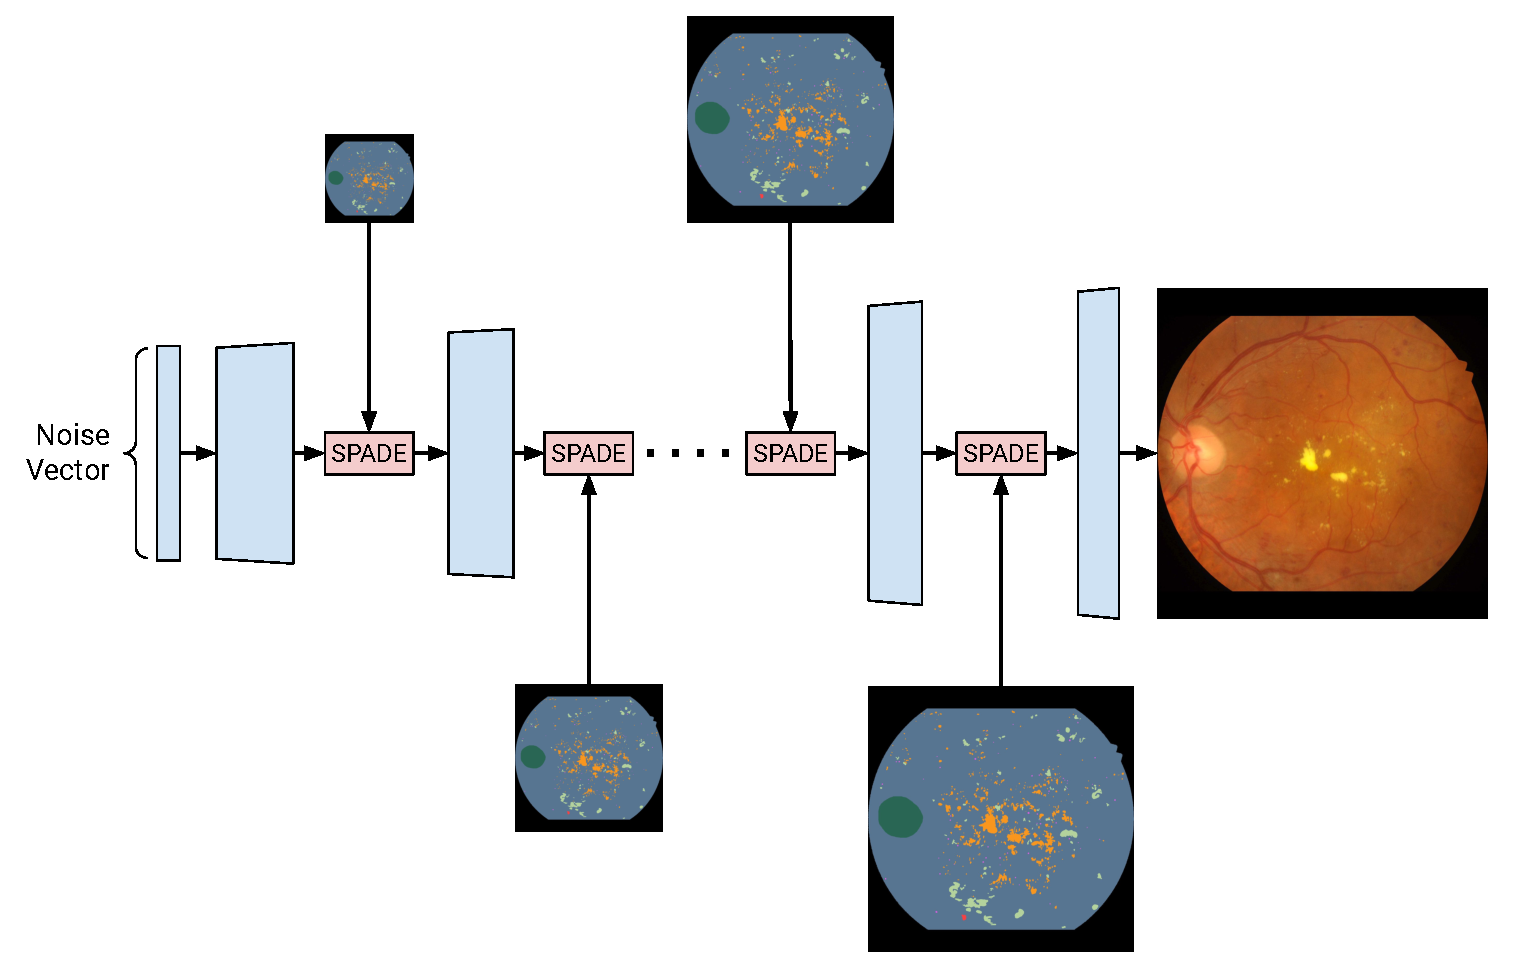
\includegraphics[width=\textwidth]{retinas/figs/spade-arch.pdf}
    \caption{Illustration of how the SPADE generator is conditioned.}
    \label{fig:spadearch}
\end{figure}

Spatially-Adaptive (De)normalisation (SPADE) is a conditional normalisation layer, like AdaIN\footnote{Interestingly, other conditional normalisation techniques such as AdaIN are actually special cases of SPADE.}, but specially crafted for the semantic image synthesis task \cite{spade}.
In SPADE, the parameters $\gamma$ and $\beta$ are now tensors instead of vectors as in AdaIN or batch normalisation. Once again, consider $X \in \mathbb{R}^{N\times C\times H\times W}$ and also the segmentation mask $M \in \mathbb{L}^{H\times W}$ where $\mathbb{L}$ is a set of integers representing the labels present in the mask. Then the SPADE transform is given by
\begin{align}
    \text{SPADE}(X, M) = \gamma_{chw}(M) \left( \frac{ X_{nchw} - \mu_c(X)}{\sigma_c(X)} \right) + \beta_{chw}(M)
\end{align}
where $\mu_c, \sigma_c$ are defined in the same way as in batch normalisation (\Cref{eq:bnmean} and \eqref{eq:bnstd}), and $\gamma_{chw}, \beta_{chw}$ denote functions that convert the segmentation map $M$ to the scalar denormalisation parameters. In practice, these functions are implemented as small convolutional networks.

Since the denormalisation parameters themselves encode enough information about the label map, we are able to discard the entire encoder part of the network in the SPADE generator.
Instead, we pass the resized segmentation map directly to the SPADE layers in the generator network, 
as depicted in \Cref{fig:spadearch}.
Note the similarity with StyleGAN in that they both inject information into conditional normalisation layers, whereas traditional GAN architectures feed information forward from the first layer.

We use the same multi-scale discriminator used in pix2pixHD.
The network is trained to translate semantic labels of resolution $512\times512$ to realistic retinal fundus images of the same size.
Weights are initialised using Xavier initialisation, and we use Hinge loss as our loss function.

Additional information is provided to the model in the form of optic disc instance maps.
Apart from these and the semantic labels, we do not provide any other form of conditioning, such as grading information.

\section{Experiments}

Experiments with this network were much more limited due to long training times and limited access to hardware.

We use the Adam optimiser with $\alpha_G = \alpha_D = 0.0002$, $\beta_1 = 0.0$, $\beta_2 = 0.9$, and a latent dimension of 256.
The network was trained for 500 epochs on two GPUs over 182 hours.

\begin{figure}[h]
    \centering
    \begin{subfigure}{0.40\textwidth}
        \centering
        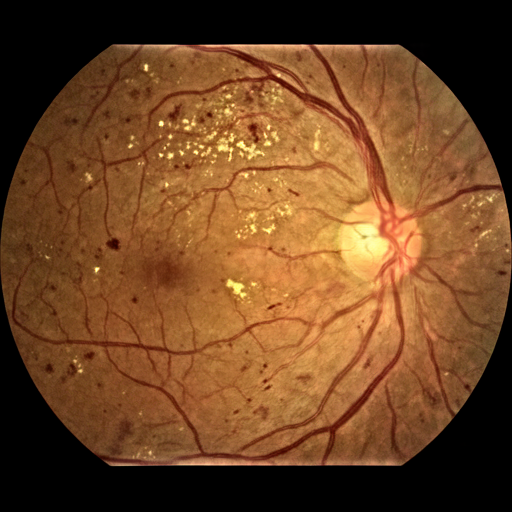
\includegraphics[width=\linewidth]{retinas/figs/no_inst.png}
        \caption{Without instance map.}
        \label{fig:without_inst}
    \end{subfigure} %
    \begin{subfigure}{0.40\textwidth}
        \centering
        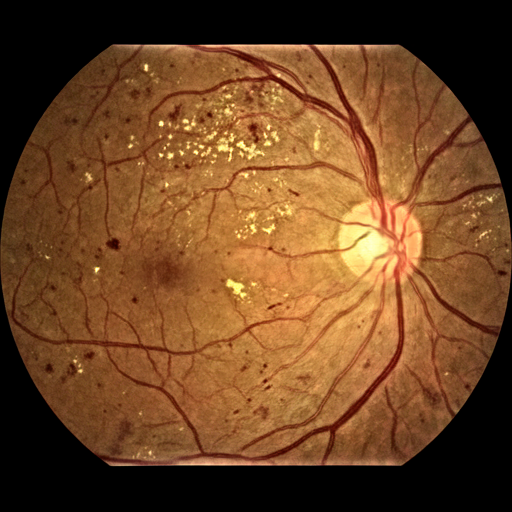
\includegraphics[width=\linewidth]{retinas/figs/with_inst.png}
        \caption{With instance map.}
        \label{fig:with_inst}
    \end{subfigure}
    \caption{Effect of instance maps.}
    \label{fig:with_without_instance}
\end{figure}

We found that the network was capable of producing realistic retina texture and structures, including blood vessels and the macula (the dark circle opposite the optic disc).
This is impressive, considering that there is no guidance for retinal structures in the semantic labels.
The network is also able to accurately place the lesions according to the semantic labels.

Layout prediction of the optic disc in particular was important for visually plausible retinas, as we found that without providing explicit conditioning in the form of instance maps the SPADE generator created images which exhibited optic discs with poorly defined boundaries.
This can be seen in \Cref{fig:with_without_instance}, where without an instance map, the optic disc is blurry and the vessels display more inconsistencies.

\subsection{Samples}

The resulting images show good diversity, with the ability to the generate different lighting conditions that were present in the source data.
A sample of images are shown in \Cref{fig:spade_sample}.

\begin{figure}[h]
    \centering
    \begin{subfigure}{0.3\textwidth}
        \centering
        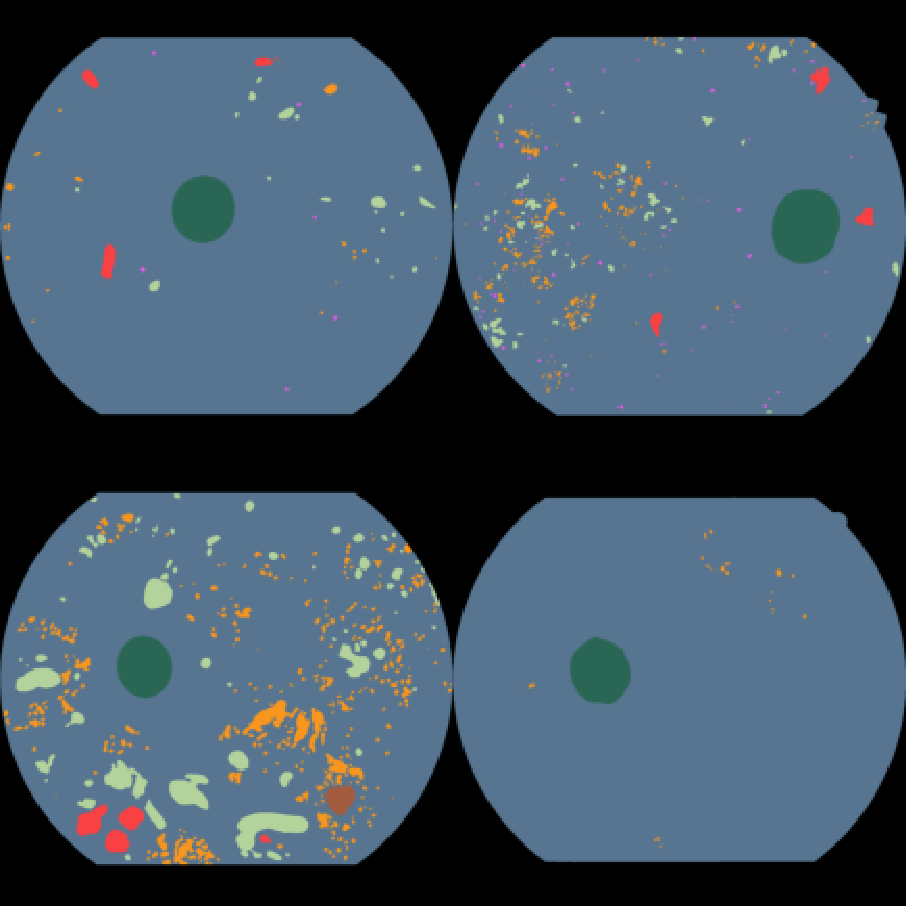
\includegraphics[width=\linewidth]{retinas/figs/spade_good_sample_labels.pdf}
        \caption{Real semantic labels.}
        \label{fig:spade_label_sample}
    \end{subfigure}
    \begin{subfigure}{0.3\textwidth}
        \centering
        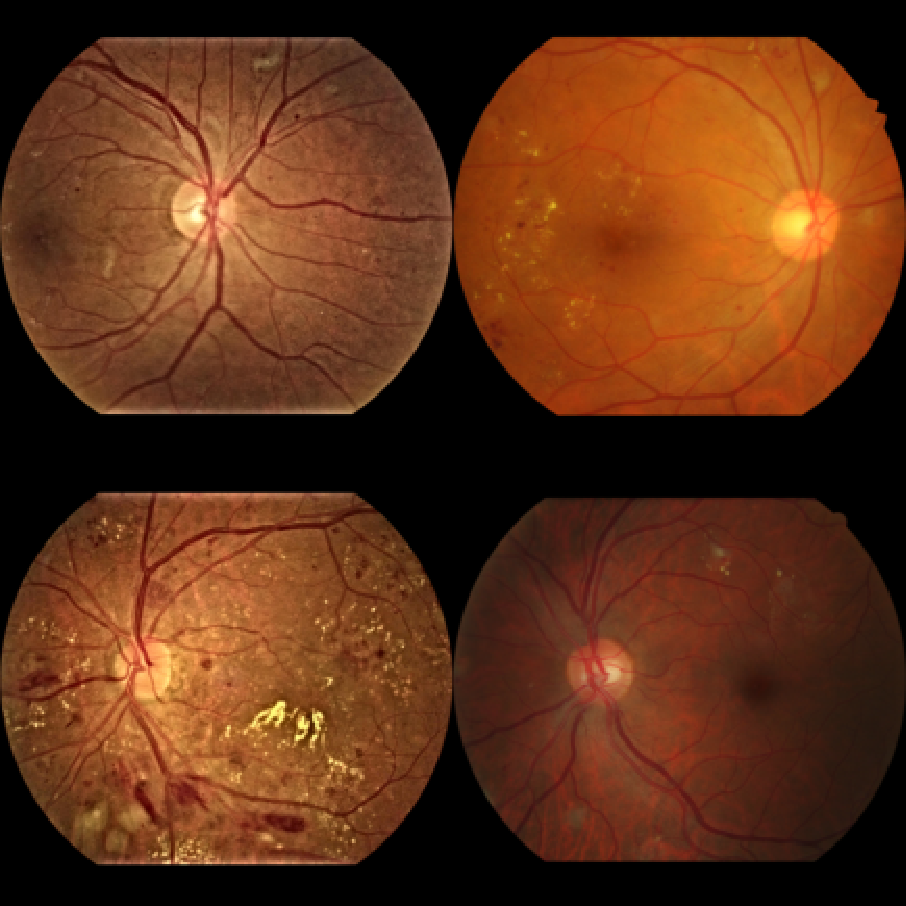
\includegraphics[width=\linewidth]{retinas/figs/spade_good_sample_images.pdf}
        \caption{Real images.}
        \label{fig:spade_image_sample}
    \end{subfigure}
    \begin{subfigure}{0.3\textwidth}
        \centering
        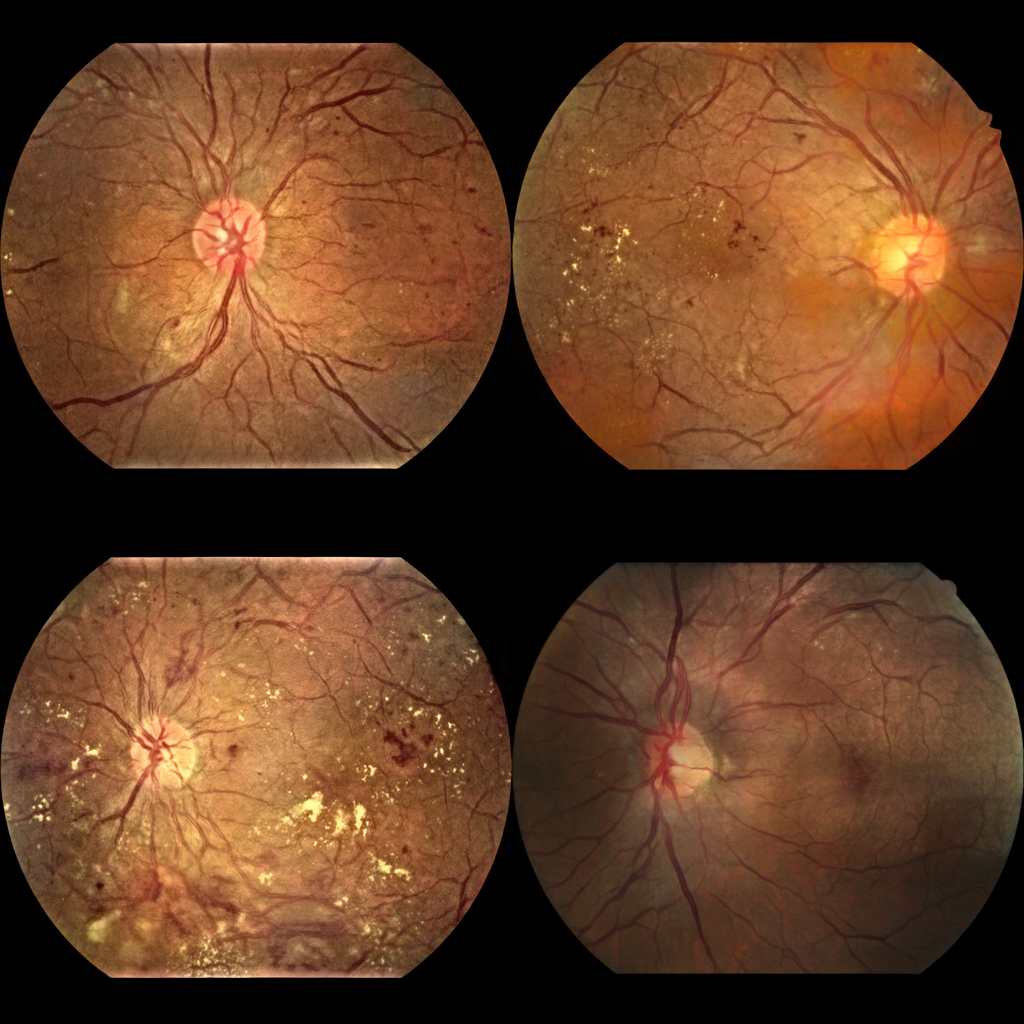
\includegraphics[width=\linewidth]{retinas/figs/spade_sample1.png}
        \caption{SPADE output.}
        \label{fig:spade_generated_sample}
    \end{subfigure}
    \caption{Comparison of real images and SPADE outputs for semantic labels from the validation set.}
    \label{fig:spade_sample}
\end{figure}

\subsection{Common Failure Modes}

\begin{figure}[h]
    \centering
    \begin{subfigure}{0.40\textwidth}
        \centering
        \includegraphics[width=\linewidth]{retinas/figs/no-od.png}
        \caption{Generated image with a misplaced vascular root.}
        \label{fig:no_od}
    \end{subfigure}
    \begin{subfigure}{0.40\textwidth}
        \centering
        \includegraphics[width=\linewidth]{retinas/figs/no-od-real.png}
        \caption{Real photograph with obscured optic disc.}
        \label{fig:no_od_real}
    \end{subfigure}
    \caption{Examples of common failure modes.}
    \label{fig:spade_bad_sample}
\end{figure}

\begin{description}
    \item[Misplaced Vascular Root] \hfill \\
    When the optic disc is not present in the semantic label, the network has difficulty placing the vascular ``root''.
    Example shown in \Cref{fig:no_od}.
    It is possible that the optic disc is obscured in a real retinal fundus photograph, as in \Cref{fig:no_od_real}, however there are only two examples of this in the training set, and the network is unable to infer that the vascular root should exist elsewhere.
    
    \item[Unrealistic Vascular Structure] \hfill \\
    Even when the optic disc is not occluded, the network sometimes generates unrealistic retinal vasculature, with non-contiguous regions.
    
    \item[Blurriness] \hfill \\
    In general, the images appear blurrier at smaller scales than the real photographs, which are sharp.
    Again, this is particularly apparently when examining the blood vessels in detail.
\end{description}

\subsection{Results}

Similarly to before, we compute the FID between the target dataset and the real training set, with results shown in \Cref{tab:spade_validation}.
The synthetic images are generated by providing SPADE with the real validation semantic labels as input to produce fake retinal fundus images as output.
Again, we also provide the FID score on the real validation retinal fundus photographs as a baseline.
We compare the original retinal fundus images, without applying illumination correction.

\begin{table}[h]
    \centering
    \begin{tabular}{lr}
        \toprule
        Configuration & FID$\downarrow$ \\
        \midrule
        Validation & 23.491 \\
        \midrule
        SPADE & 48.438 \\
        + instance maps & \textbf{46.603} \\
        \bottomrule
    \end{tabular}
    \caption{FID scores between real images from the training set and the output of SPADE on the real validation semantic labels. Best results for each metric in bold (excluding the baseline).}
    \label{tab:spade_validation}
\end{table}

This shows that the use of instance maps yield a small improvement in overall image quality.
Unfortunately, since we are not able to obtain the code for DR-GAN or Tub-sGAN, and since the authors did not state the dimensionality used to compute the FID scores reported in their papers (which can alter the score by orders of magnitude), it's impossible to draw a quantitative comparison.
Instead, we leave this as future work.

\chapter{Evaluation} \label{cha:evaluation}

In \Cref{cha:labels} and \Cref{cha:retinas}, we examined the quality of generation of each part of the system in isolation.
Having having done this, we return to the overarching goal of this project: to observe the effect of \emph{fully-synthetic} data (i.e. generated retinas from generated semantic labels) on downstream tasks.
Hence, in the evaluation phase we aim to answer the following questions:
\begin{itemize}
    \item How closely does synthetic data resemble the real data?
    \item What effect does synthetic data have on lesion segmentation performance?
    \item What effect does synthetic data have on grading performance?
\end{itemize}

\section{Preliminary Results} \label{sec:prelim}

An early version of this project was submitted as a short paper\footnote{What qualifies as a ``short paper'' can be found at \url{https://2021.midl.io/call-for-papers.html}.} to MIDL 2021.
While using similar techniques, this work focused on generation of only the optic disc and hard exudate lesions, with the retina being added afterwards using a circle mask, in the same way as discussed above.
These preliminary results were promising, and showed that inflating real data with synthetic data was successful in improving the performance of semantic segmentation for lesions.

Despite this, the results of the paper were limited in that restricting the problem domain in this way made the task far easier, and naturally allowed for more stable training.
This was not only reflected in the generated image quality, in that the GAN was able to generate more plausible semantic labels, but also in the level of conditioning.
Here, we extend those models to generate 9 classes (from 3), and provide a more complete evaluation.

\section{Visual Quality}

\begin{figure}[h]
    \centering
    \begin{subfigure}{0.31\textwidth}
        \centering
        \includegraphics[width=\linewidth]{evaluation/figs/acgan_retina_sample.pdf}
        \caption{ACGAN}
        \label{fig:generated_retinas_acgan}
    \end{subfigure}
    \begin{subfigure}{0.31\textwidth}
        \centering
        \includegraphics[width=\linewidth]{evaluation/figs/progan_retina_sample.pdf}
        \caption{ProGAN}
        \label{fig:generated_retinas_progan}
    \end{subfigure}
    \begin{subfigure}{0.31\textwidth}
        \centering
        \includegraphics[width=\linewidth]{evaluation/figs/copypaste_retina_sample.pdf}
        \caption{Copy-Paste}
        \label{fig:generated_retinas_copypaste}
    \end{subfigure}
    \caption{Fully-synthetic retinal fundus images.}
    \label{fig:generated_retinas}
\end{figure}

We begin by qualitatively and quantitatively evaluating the overall visual quality of the fully-synthetic images.
A sample of images, created using each semantic label generation method, are shown in \Cref{fig:generated_retinas}.
For all experiments in this evaluation, we use the ACGAN and ProGAN generated samples without any fundus masking, unless otherwise specified.
The semantic labels are translated into retinal fundus images using the same trained SPADE network for each method with instance maps.

Curiously, images that have few lesions resemble photographs taken from the e-ophtha dataset most closely.
This is likely because most photographs of healthy retinas come from the e-ophtha dataset, and this bias is reflected in the output of the SPADE network, highlighting the need for greater diversity in the source data.

To quantify differences in diversity and quality, we begin by generating 3000 samples of fully-synthetic images in equal proportions across the five DR grades using each of the methods.
We then compute the FID score between these and the retinal fundus photographs from the training set, with results shown in \Cref{tab:spade_generated}. 
We are particularly interested in how these compare in relation to real images; to this end, the FID between the real training set and real validation/test sets are also given.

Surprisingly, the images who had their retina boundaries masked post-generation performed worse than their unmodified counterparts -- despite them performing better in the semantic label evaluation.
The reason for this is not entirely clear, but we can put forward a couple of theories.
One possible reason is that the FID score is simply not designed for these types of images, and thus gives spurious results that would be inconsistent with human perception.
In particular, purely geometric shapes such as the circle that forms the retinal fundus boundary are rare in the real world, and could be thought of as ``unnatural''.
Moreover, in the masked images these boundaries are only ever perfect circles, whereas in the source dataset, samples whose top and bottom sections have been cropped are common, which could cause distance between the data distributions.

\begin{table}[h]
    \centering
    \begin{tabular}{lrr}
        \toprule
        Configuration & \multicolumn{2}{r}{FID$\downarrow$} \\
        \midrule
        Test & 23.281 & \\
        Validation & 23.491 & \\
        \midrule
        ACGAN & \textbf{43.042} & $\pm$ 0.196 \\
        + mask & 50.642 & $\pm$ 0.229 \\
        \midrule
        ProGAN & 48.882 & $\pm$ 0.305 \\
        + mask & 54.353 & $\pm$ 0.092 \\
        \midrule
        Copy-Paste & 45.394 & $\pm$ 0.072 \\
        \bottomrule
    \end{tabular}
    \caption{FID scores between real images from the training set and the output of SPADE on the generated semantic labels. We report the mean of three runs and the standard error of the mean. Raw data can be found in \Cref{cha:raw_data}. Best results for each metric in bold (excluding the baseline).}
    \label{tab:spade_generated}
\end{table}

\section{Classification Performance}

The intuition for the first part of our classification performance evaluation is that images that closely resemble their source class should be able to be labelled correctly by a classifier trained on real data. 
To quantify this, we use the standard precision, recall, and $F_1$ score metrics.

Next, we investigate two different approaches to using synthetic data \emph{together} with real data to augment model performance.
In the first, we train models on a mix of real and generated data.
As part of this, we investigate the effects that varying the amount of synthetic data used, in terms of the proportion of the training data which is synthetic, has on the final model performance.
Each experiment will use the entire set of real training data, and only the amount of synthetic data will be tuned.
From the generated data, we sample the appropriate number of images according to the experiment, and concatenate this with the real training data.
\Cref{tab:synthetic_proportions_classification} shows how much synthetic data is used in each classification experiment -- note how for these experiments, we use the smaller grading set instead of the EyePACS dataset, since EyePACS is extremely large and therefore slow to train on.
We also considered an alternative approach where we simply take a small subset of the EyePACS dataset, but we found that the class imbalance and high amount of noise in the parent dataset (which would usually be offset by the large volume of data) caused extremely poor performance on the test set.

\begin{table}[h]
    \centering
    \begin{tabular}{rrrr}
       \toprule
       \# Real & \% Synthetic & \# Synthetic & \# Total \\
       \midrule
       \multirow{3}*{1606} & 25 & 535 & 2141 \\ 
       & 50 & 1606 & 3212 \\ 
       & 75 & 4818 & 6424 \\ 
       \bottomrule
    \end{tabular}
    \caption{Data amounts for classification experiments.}
    \label{tab:synthetic_proportions_classification}
\end{table}

The second approach is related to transfer learning.
In this particular version of the technique, we will pre-train a network on only synthetic data (7000 images) for 100 epochs, and then subsequently fine-tune on only real data for a further 100 epochs.
We are interested in determining what the effect is on both how fast the model improves on real data, and if the final performance is changed.
To contrast and compare the merits of both approaches, we collect performance metrics on the test set for each configuration, and compare these against a model trained on real data only.

Our classification network is a ResNet-50 trained to classify $512\times 512$ illumination-corrected retinal fundus images as one of the five DR grades.
Across all experiments, the network is trained for 100 epochs (where training loss plateaued) with learning rate $\alpha = 0.001$, and batch size 16, on a mix of single Nvidia Titan X Pascal and Nvidia GeForce GTX 1080 GPUs.
Each configuration is trained from scratch, with the exception of the fine-tuning stage of the transfer learning experiment.
We refer to models trained on real data only as ``baseline'' models.

\subsection{Results}

\begin{table}[h]
    \centering
    \begin{tabular}{lrrrrr}
    \toprule
        Configuration & Accuracy$\uparrow$ & Precision$\uparrow$ & Recall$\uparrow$ & $F_1$$\uparrow$ & $\kappa$$\uparrow$ \\
    \midrule 
    Validation & 0.517 & 0.455 & 0.437 & 0.435 & 0.569 \\
    Test & 0.509 & 0.442 & 0.441 &0.430 & 0.539 \\
    \midrule
        ACGAN & 0.202 & 0.196 & 0.201 & 0.164 & $-0.006$ \\
    \midrule
        ProGAN & 0.199 & 0.216 & 0.200 & 0.159 & $-0.002$ \\
    \midrule
        Copy-Paste & \textbf{0.313} & \textbf{0.366} & \textbf{0.313} & \textbf{0.247} & \textbf{0.315} \\
    \bottomrule
    \end{tabular}
    \caption{Performance of a classification model trained with only real data on real and synthetic datasets. Mean of three runs, raw data can be found in \Cref{cha:raw_data}. Best results for each metric in bold (excluding the baseline).}
    \label{tab:classification_performance}
\end{table}

The results of the real classifier on synthetic data are shown in \Cref{tab:classification_performance}.
These figures are somewhat surprising, with all types of synthetic data unable to be well-classified by the ResNet.
We expected that the copy-paste generated data would perform best out of the synthetic datasets, since its semantic labels were able to be accurately classified (\Cref{tab:acgan_results}), and this expectation is confirmed by the data.
However, even if copy-paste generated data performed the best out of the synthetic datasets, it performs poorly relative to the real validation and test sets.
Since the semantic labels of copy-pasted data were able to be classified well, it could be that performance here is being bottlenecked by the image-to-image translation portion of the generation process.

\begin{table}[h]
    \centering
    \begin{tabular}{lrr@{}lr@{}lr@{}lr@{}lr@{}l}
    \toprule
        Configuration & \% Synthetic & Accuracy$\uparrow$ & & Precision$\uparrow$ & & Recall$\uparrow$ & & $F_1$$\uparrow$ & & $\kappa$$\uparrow$ & \\
    \midrule
    Real & 0 & 0.509 & & 0.442 & & 0.441 & & 0.430 & & 0.539 & \\
    \midrule
    \multirow{3}*{ACGAN} & 25 & 0.400 & & 0.440 & & 0.366 & & 0.324 & & 0.292 & \\
                         & 50 & 0.428 & & 0.467 & * & 0.414 & & 0.366 & & 0.328 & \\
                         & 75 & 0.386 & & 0.338 & & 0.302 & & 0.253 & & 0.281 & \\
    \midrule
    \multirow{3}*{ProGAN} & 25 & 0.519 & * & 0.491 & * & 0.506 & * & 0.477 & * & 0.631 & * \\
                          & 50 & 0.410 &   & 0.470 & * & 0.436 & & 0.360 & & 0.525 & \\
                          & 75 & 0.570 & * & 0.487 & * & 0.409 & & 0.395 & & 0.489 & \\
    \midrule
    \multirow{3}*{Copy-Paste} & 25 & 0.502 & & 0.462 & * & 0.479 & * & 0.448 & * & 0.607 & * \\
                              & 50 & 0.561 & * & \textbf{0.533} & * & \textbf{0.566} & * & \textbf{0.522} & * & \textbf{0.721} & * \\
                             & 75 & \textbf{0.599} & * & 0.522 & * & 0.536 & * & 0.511 & * & 0.703 & * \\
    \bottomrule
    \end{tabular}
    \caption{Performance of a classification model trained with mixed data on the test set. Mean of three runs, raw data can be found in \Cref{cha:raw_data}. Best results for each metric in bold (excluding the baseline), and improvements on the baseline are marked with *.}
    \label{tab:classification_mixed_performance}
\end{table}

Next, we conduct experiments by training the classifier on a mix of real and synthetic data, with results shown in \Cref{tab:classification_mixed_performance}.
This set of results are less surprising, with the ACGAN unanimously causing classification performance to drop.
A small amount of synthetic data generated from the ProGAN appears to be beneficial, slightly boosting the classification metrics at 25\% synthetic data, above which performance begins to fall.
Meanwhile, training on a mix of real and copy-pasted data is able to significantly boost classification performance.
What is most noteworthy here is how copy-pasted data can increase performance by a large margin when mixed with real data, yet is not able to be accurately classified by a model trained on only real data.
Both the ACGAN and copy-paste configurations observe a peak at 50\% synthetic data, with 25\% and 75\% performing worse.
This suggests that increasing the amount of synthetic data will improve model performance to a critical point, after which the model with begin to overfit to unrealistic features in the synthetic data.
The models used in these experiments were trained over between one and eleven hours each, depending on the size of the training set.

\begin{table}[h]
    \centering
    \begin{tabular}{llr@{}lr@{}lr@{}lr@{}lr@{}l}
    \toprule
        \multicolumn{2}{c}{Configuration} & Accuracy$\uparrow$ & & Precision$\uparrow$ & & Recall$\uparrow$ & & $F_1$$\uparrow$ & & $\kappa$$\uparrow$ & \\
    \midrule
    Real & & 0.509 & & 0.442 & & 0.441 & & 0.430 & & 0.539 & \\
    \midrule
    \multirow{2}*{Copy-Paste} & Pre-Trained & \textbf{0.605} & * & \textbf{0.559} & * &  \textbf{0.534} & * & \textbf{0.529} & * & \textbf{0.694} &* \\
               & Fine-Tuned & 0.566 & * & 0.555 & * & 0.525 & * & 0.512 & * & 0.660 & * \\
    \bottomrule
    \end{tabular}
    \caption{Performance of a classification model on the test set before and after fine-tuning. Mean of three runs, raw data can be found in \Cref{cha:raw_data}. Best results for each metric in bold (excluding the baseline), and improvements on the baseline are marked with *.}
    \label{tab:classification_transfer}
\end{table}

Finally, we look at how transfer learning affects the ability of the model to classify images correctly.
We only use copy-pasted data for pre-training since it appears to be most effective for this task, and the results of these experiments are shown in \Cref{tab:classification_transfer}.
Here, ``pre-trained'' refers to the network once it has finished training on only synthetic data, and ``fine-tuned'' refers to the same network once it has finished further training on real data.
The results are unexpected, with the synthetic-only model performing \emph{better} on the test set than the fine-tuned network.
A possible explanation for this is that the real dataset is small, and has noisy DR severity labels.
Images generated by copy-pasting are the result of sampling semantic labels from multiple different images of the same grade, causing the classes to be more robust, and therefore less noisy.
Both the pre-trained and fine-tuned networks perform better than training on only real data, which implies that pre-training increases the ability of the model to extract useful features.
The pre-trained model is able to outperform the baseline and fine-tuned models, but its $\kappa$ falls short of the copy-paste mixed-data training approach, despite having a slightly more favourable $F_1$ score.
This is a consequence of the quadratic weighting used to calculate $\kappa$, but we maintain use of $\kappa$ as the determining factor of ``overall'' performance.

It is also interesting to analyse the resulting loss curves of transfer learning, and to compare these against the losses of a network trained on only real data, as shown in \Cref{fig:classification_transfer_loss}.
The loss in the pre-training stage decreases slowly, which makes sense since the greater volume of synthetic data (which could be thought of as a type of data augmentation) has a regularising effect on training.
Once the network enters the fine-tuning stage, the model is able to leverage its past experience, and begins training at a much lower loss than the one trained from scratch.
Despite this ``head-start'', the baseline model's loss decreases quickly, and by the end of training is approximately the same magnitude as the fine-tuned network.
The effect of transfer learning on the validation loss is more subtle, and there is no clear difference between the losses of the baseline and fine-tuned models.

\begin{figure}[h]
    \centering
    \begin{subfigure}{0.45\textwidth}
        \centering
        \includegraphics[width=\linewidth]{evaluation/figs/transfer_training_loss.pdf}
        \caption{Training loss.}
        \label{fig:classification_transfer_loss_training}
    \end{subfigure}
    \begin{subfigure}{0.45\textwidth}
        \centering
        \includegraphics[width=\linewidth]{evaluation/figs/transfer_validation_loss.pdf}
        \caption{Validation loss.}
        \label{fig:classification_transfer_loss_validation}
    \end{subfigure}
    \caption{Loss curves for transfer learning. Solid lines are the means of three runs, and the shaded regions show the minimum and maximum values.}
    \label{fig:classification_transfer_loss}
\end{figure}

\section{Segmentation Performance}

\begin{table}[h]
    \centering
    \begin{tabular}{rrrr}
       \toprule
       \# Real & \% Synthetic & \# Synthetic & \# Total \\
       \midrule
       \multirow{3}*{1607} & 25 & 536 & 2143 \\ 
       & 50 & 1607 & 3214 \\ 
       & 75 & 4821 & 6428 \\ 
       \bottomrule
    \end{tabular}
    \caption{Data amounts for segmentation experiments.}
    \label{tab:synthetic_proportions_segmentation}
\end{table}

Applying a similar principle to the segmentation task: if our model produces clear and well-conditional retinal fundus images with precise segmentation maps, a model should be able to segment our synthesised images about as well as it can segment real images. 
We then go on to investigate the same two approaches to training on synthetic data as described in the previous section.
For the mixed-data approach, we use use the proportions specified in \Cref{tab:synthetic_proportions_segmentation}.

A standard U-Net is used as our segmentation model architecture.
Models were trained to segment all six lesion types (microaneurysms, haemorrhages, hard exudates, soft exudates, intraretinal microvascular abnormalities, and neovascularistion) at a resolution of $512 \times 512$.
They do not segment other structures such as the optic disc or fundus boundary.
All models were trained for 50 epochs with a learning rate of $\alpha = 0.0005$ and batch size of 4 on a mix of single Nvidia Titan X Pascal and Nvidia GeForce GTX 1080 GPUs.
We focus on the \emph{relative} performance as opposed to the absolute performance, and therefore do not spend time optimising the model hyperparameters.

\subsection{Results}

\begin{table}[h]
    \centering
    \begin{tabular}{lrrr}
    \toprule
        Configuration & Precision$\uparrow$ & Recall$\uparrow$ & $F_1$$\uparrow$ \\
    \midrule 
    Test & 0.710 & 0.400 & 0.439 \\
    Validation & 0.690 & 0.374 & 0.434 \\
    \midrule
        ACGAN & 0.662 & 0.200 & 0.278 \\
    \midrule
        ProGAN & 0.754 & 0.183 & 0.523 \\
    \midrule
        Copy-Paste & \textbf{0.808} & \textbf{0.462} & \textbf{0.527} \\
    \bottomrule
    \end{tabular}
    \caption{Performance of a segmentation model trained with only real data on real and synthetic datasets. Mean of three runs, raw data can be found in \Cref{cha:raw_data}. Best results for each metric in bold (excluding the baseline).}
    \label{tab:segmentation_performance}
\end{table}

\Cref{tab:segmentation_performance} shows the results of running the baseline segmentation model trained with real data on the synthetic datasets.
We find that the model performs best across all metrics on the copy-pasted data, followed closely by the ProGAN.
The overall performance (as determined by the $F_1$ score) for both of these models is greater than that of the test and validation sets.
This is indicative of plausible generated semantic labels and well-conditioned image-to-image translation.
Performance on the ACGAN generated data, however, is significantly poorer than for any other dataset.

\begin{table}[h]
    \centering
    \begin{tabular}{lrr@{}lr@{}lr@{}l}
        \toprule
        Configuration & \% Synthetic & Precision$\uparrow$ & & Recall$\uparrow$ & & $F_1$$\uparrow$ & \\
        \midrule
        Real & 0 & 0.710 & & 0.400 & & 0.439 & \\
        \midrule
        \multirow{3}*{ACGAN} & 25 & 0.688 & & 0.368 & & 0.421 & \\
              & 50 & 0.608 & & 0.353 & & 0.406 & \\
              & 75 & \textbf{0.723} & * & 0.412 & * & 0.473 & * \\
        \midrule
        \multirow{3}*{ProGAN} & 25 & 0.687 & & 0.400 & & 0.449 & *\\
               & 50 & 0.662 & & \textbf{0.482} & * & 0.464 & * \\
               & 75 & 0.685 & & 0.406 & * & 0.461 & * \\
        \midrule
        \multirow{3}*{Copy-Paste} & 25 & 0.716 & * & 0.297 & & 0.364 & \\
                   & 50 & 0.702 & & 0.392 & & 0.452 & * \\
                   & 75 & 0.689 & & 0.423 & * & \textbf{0.476} & *\\
        \bottomrule
    \end{tabular}
    \caption{Performance of a segmentation model trained with mixed data on the test set. Mean of three runs, raw data can be found in \Cref{cha:raw_data}. Best results for each metric in bold (excluding the baseline), and improvements on the baseline are marked with *.}
    \label{tab:segmentation_mixed_performance}
\end{table}

Turning our attention to experiments conducted with mixed training data, \Cref{tab:segmentation_mixed_performance} shows the performance of the segmentation model trained under varying amounts of synthetic data.
The results are extremely promising, showing that segmentation performance can be boosted by training on synthetic data.
We identify an interesting trend where increasing the amount of synthetic data simultaneously decreases precision while increasing recall.
The overall effect of this is that the $F_1$ score improves, at least up to 75\% synthetic data. 
We can think of precision as ``how many selected items are relevant`` and recall as ``how many relevant items are selected''; hence, decreased precision and increased recall can be interpreted as the resulting model being more ``liberal'' with its selection.
It's likely that, as with the classification experiments, this relationship reaches a point where the $F_1$ score begins to decrease, but further experiments are required to verify this. 

\begin{table}[h]
    \centering
    \begin{tabular}{llr@{}lr@{}lr@{}l}
        \toprule
        \multicolumn{2}{c}{Configuration} & Precision$\uparrow$ & & Recall$\uparrow$ & & $F_1$$\uparrow$ & \\
        \midrule
        Real & & 0.710 & & 0.400 & & 0.439 & \\
        \midrule
        \multirow{2}*{Copy-Paste} & Pre-Trained & 0.646 & & \textbf{0.453} & * & \textbf{0.510} &* \\
               & Fine-Tuned & \textbf{0.729} & * & 0.420 & * & 0.501 & * \\
        \bottomrule
    \end{tabular}
    \caption{Performance of a segmentation model on the test set before and after fine-tuning. Mean of three runs, raw data can be found in \Cref{cha:raw_data}. Best results for each metric in bold (excluding the baseline), and improvements on the baseline are marked with *.}
    \label{tab:segmentation_transfer_performance}
\end{table}

This trend continues with the transfer learning approach, where the pre-trained network exhibits a higher recall but lower precision than the baseline model, with a greater overall $F_1$ score.
Conversely, continuing training on the real data has the inverse effect of increasing precision and decreasing recall.
Again, we see parallels with the transfer learning approach applied to classification in that the $F_1$ score is better on the pre-trained model than the fine-tuned model, as if seeing real data causes performance to drop.
Both the pre-trained and fine-tuned models are able to achieve a greater $F_1$ score than any of the baseline or mixed-data training approaches, suggesting that this is the optimal strategy to maximise segmentation performance.

Looking at the loss curves in \Cref{fig:segmentation_transfer_loss}, we see a similar pattern to the classification transfer learning loss, although training loss actually increases when entering the fine-tuning stage, suggesting the model has overfit on the synthetic data.

\begin{figure}[h]
    \centering
    \begin{subfigure}{0.45\textwidth}
        \centering
        \includegraphics[width=\linewidth]{evaluation/figs/segmentation_transfer_training_loss.pdf}
        \caption{Training loss.}
        \label{fig:segmentation_transfer_loss_training}
    \end{subfigure}
    \begin{subfigure}{0.45\textwidth}
        \centering
        \includegraphics[width=\linewidth]{evaluation/figs/segmentation_transfer_validation_loss.pdf}
        \caption{Validation loss.}
        \label{fig:segmentation_transfer_loss_validation}
    \end{subfigure}
    \caption{Loss curves for transfer learning, plotted on a logarithmic scale. Solid lines are the means of three runs, and the shaded regions show the minimum and maximum values.}
    \label{fig:segmentation_transfer_loss}
\end{figure}
\chapter{Conclusion}

In this project, we have shown that semantic generation of retinal fundus images is viable as a method of data augmentation, and shows great potential in improving the performance downstream tasks.
First, we provided a survey of available datasets and their properties.
To expand our training data, we showed how weak supervision can be used to inflate the training set in low-data regimes.
We then introduced a novel two-step process for the synthesis of realistic retinal fundus images with accompanying semantic labels, conditioned on DR severity.
Finally, we showed that using synthetic data as a basis for mixed-data training or transfer learning can increase the performance of segmentation and classification models on real data.

\section{Limitations}

While it remains true that there is no better substitute for high-quality annotated data, we have shown that synthetic data and its application to medical imaging is a promising avenue of research.
However, it should be noted that this project presents only an early proof-of-concept, and as such exhibits a number of limitations.

Despite the fact that the images used in these experiments were of relatively low resolution when compared to raw images captured by cameras, generation of high-resolution, natural, medical images has already been shown to be feasible \cite{mammogan}.
However, it remains unclear how the same can be reliably done for the generation of sparse semantic labels.
This work suggests that DCGAN-based architectures are ill-suited for this task, and that progressive growing is the key to yielding improved results.

While we were successful in enhancing model performance, there remains much room for improvement in terms of the quality of generated images.
Having seen impressive results on natural looking images, it would be exciting to bring semantic label generation GANs up to parity.
A synthetic data generator can be considered to rely on two major factors, either of which can become a bottleneck: the quality of input data; and the capacity of the model to learn the representation of the data distribution.
There are multiple facets that determine the ``quality'' of training data, the most obvious being simply the volume.
In our case, having less than 2000 training images, and further subdividing this set due to conditioning, makes it difficult to learn a general representation without overfitting.
To test this, we could train the GANs on a large volume of copy-paste generated data, with the goal not necessarily being to generate anatomically correct retinal fundus images, but rather to see if increasing the amount of available data allows a GAN to better represent the images.
Otherwise, if this is not the case then we can identify that the representational power of the generator or discriminator architecture simply is not great enough.

Moreover, the quality of annotations available to us presented an issue.
Many datasets are missing the annotations we needed for these tasks, and other datasets simply have annotations which are too coarse.
Not only is the accuracy and precision in the labels of the training data important, but also the diversity of data.
Changes in imaging conditions, such as field-of-view, focal length, and lighting, can cause differences between the training and production data.
Since generative models aim to create data points which are plausibly sampled from the input distribution, this covariate shift may cause the models trained on synthetic data to not be robust to all field conditions, and therefore produce spurious results.

Finally, there are a number of caveats inherent to the use of synthetic data.
The generative models presented in this work provide no guarantee on the validity or anatomically correctness of generated data.
Hence, the model may be susceptible to producing anomalous results, and a downstream model which incorrectly learns these features will reflect this.
One must also be aware that over-training on synthetic data can cause a model to overfit to unrealistic features in the synthetic data.

\section{Future Work}

In this work, we generated synthetic data that had ``annotations'' for both the segmentation and classification task.
We then evaluated the two tasks separately.
Yet, methods for joint classification and segmentation of the retinal fundus modality exist in the literature \cite{ynet}, so supplying these models with the synthetic samples could be an interesting study, and may improve performance by a greater margin than on each individual task separately.

When conditioning our models, did not incorporate retinal structures such as the vasculature or location of the macula. 
Instead, these details were generated by the SPADE network.
However, these structures potentially contain important anatomical information; for example, the proximity of lesions to the macula may inform the severity of disease.
Incorporating these conditions could further guide and inform the generation of semantic labels.

While thorough, the evaluation for this project was limited to ad-hoc metrics for measuring GAN performance, which may not be entirely appropriate, and so there are a number of improvements that could be made here.
We have discussed how the FID is not ideal for quantifying the quality of retinal fundus images or semantic labels.
It's possible that new metrics must be developed for these modalities -- this could possibly be as simple as training the Inception network used to calculate the FID on retinal fundus images.
Also, we were unable to secure any human experts for this project, meaning we cannot draw any concrete conclusions about the anatomical correctness of generated images.
Further applications not explored here include use in training human experts to better identify retinal lesions, for which we would need highly plausible images.

A large part of this work emphasises the difficulty of training GANs in a stable manner.
While it is generally accepted that GANs lead the state-of-the-art in terms of high-fidelity image generation, other advances in generative models such as VAEs and autoregressive models show potential, bringing into question whether GANs are necessarily the most suitable framework for this use-case.
One considerable advantage that these techniques have is that training is much more stable, and going forward it is well-worth exploring whether equal or greater quality semantic labels can be synthesised by these models.

\section{Ethical Issues} \label{sec:ethics}

In this section, we discuss the potential implications of deploying an automated decision-making system in the context of medicine.

\subsection{Machine Learning in Healthcare}

Machine learning techniques and their application to healthcare have see massive popularity in the past decade, largely thanks to their versatility and ability to achieve groundbreaking results.
The use of artificial intelligence in medicine goes back as far as the 1960s \cite{dendral}, but what sets machine learning apart is its ability to learn directly from large amounts of data, instead of relying on hard-coded rules.

As a result, the usefulness of a machine learning model is bounded by the quality of its training data.
Hence, it is of massive importance that the source data is as free of bias as possible, as prejudice in the training data will translate to prejudice in the decisions that the model makes.
This is not just a hypothetical, but a very real problem that has been demonstrated time and time again.
For instance, in \citeyear{Obermeyer447} \citeauthor{Obermeyer447} \cite{Obermeyer447} found evidence of gross racial bias in a commercial AI system used in the U.S healthcare system.
A similar risk is present in our domain since skin tone affects fundus pigmentation, and the prevalence of ocular diseases has been shown to vary between ethnicities \cite{bourne2011}.
By deliberately sampling an unbalanced subset from the EyePACS dataset, \citeauthor{burlina2020addressing} \cite{burlina2020addressing} was able to show a significant disparity based on skin-tone in the performance of a DR classification model, when trained on unbalanced data.
In our case, data bias is likely since the little data we have is collated from local hospitals, decreasing the chance of a diverse and balanced dataset, and we cannot afford to selectively undersample our data.
The consequence of this is that a synthetic data generator trained on biased data will naturally generate more data reflecting that bias, exacerbating the issue.
\citeauthor{burlina2020addressing} proposed an effective method of debiasing the source data by applying StyleGAN to generate fundus images which are then manipulated in the latent space to exhibit different skin tones.
A similar idea could be interesting to explore as an extension to this project.

\subsection{Data Privacy}

Diabetic retinopathy is not a rare disease, and the precise locations from which the patient data was collected is not given in any of the used datasets.
Applying the ``motivated intruder'' test \cite{ico}, it is clear that individuals will not be directly or indirectly re-identifiable from the retina images.
Since there is no identifying information accompanying the retinal fundus photographs in any of our datasets, and an individual cannot (practically) be identified from a retinal fundus image, we consider our data to be ``truly anonymised'', as defined under Retical 26 of the GDPR \cite{gdpr}.

\subsection{Copyright and Licensing}

To ensure that the contributions of this project are as as freely available as possible, any software will be distributed under a permissive FOSS license.
Proper attribution is desirable, making the (3-clause) BSD license the natural choice.
Since BSD only covers source code, we license other work (images, documentation, etc.) under CC BY 4.0 which is similar to BSD in spirit.
An additional complication is that copyright and licensing only covers works created by humans.
However, since a degree of human creative input did go into creating the synthetic data generator, it's reasonable to put these under the same license.
In terms of using third-party software, we must take care to retain the copyright notices of PyTorch\footnote{\url{https://github.com/pytorch/pytorch/blob/master/LICENSE}} and any other software that uses a similar license. 
This project will not be applied commercially, so we are free to use works licensed under non-commercial licenses such as SPADE\footnote{\url{https://github.com/NVlabs/SPADE/blob/master/LICENSE.md}}.
\appendix

\chapter{Supplementary Materials} \label{cha:supp}

\begin{description}
\item[Codebase] \url{https://github.com/semantic-retina/semantic-retina-generation}
\item[Materials] \url{https://github.com/semantic-retina/supplementary-materials}
\end{description}

\section{FGADR Exclusion List} \label{sec:fgadr_excl}

This is a list of files that we determined too coarse to be used as segmentation maps, and were therefore excluded from our training data.
It can be found in CSV format in the supplementary materials repository under \lstinline{data/fgadr_denylist.csv}.

\section{Optic Disc Annotations} \label{sec:od}

For this project, we manually annotated the optic discs for the FGADR and DiaRetDB1 datasets.
This was done using the open-source Make Sense annotation tool\footnote{\url{https://www.makesense.ai}}, and are stored as JSON files under the \lstinline{data} directory.
Utilities for pre-processing datasets using these files are included in the main code repository.
Inferred annotations for e-ophtha were collected as detailed in \Cref{sec:optic_disc_inference}, and are stored as PNG files containing binary masks under the \lstinline{data/eophtha_od} directory.

\section{Models} \label{sec:models}

For reproducibility, the supplementary materials repository contains all model weights used in this project, including the ACGAN, ProGAN, ResNet, and U-Net.
These are contained under the \lstinline{models} directory.

\section{Raw Data} \label{cha:raw_data}

Raw data collected from experiments can be found as spreadsheet files under the \lstinline{raw data} directory.

\section{Mask Overlay Tool}
\begin{description}
\item[Mask Overlay Tool] \url{https://github.com/semantic-retina/mask-overlay}
\end{description}

The mask overlay tool is a small command-line program built to create labelled retinal fundus image diagrams, such as \Cref{fig:lesions}. 

% \chapter{Ethics Checklist}
% \Cref{tab:ethicschecklist} presents an abridged version of the \emph{Ethics Checklist} provided by the Department of Computing. Issues identified in the checklist are discussed in \Cref{sec:ethics}.
% 
% \begin{longtable}{p{0.01\textwidth}>{\raggedright}p{0.85\textwidth}r}
% \toprule
%    \multicolumn{2}{l}{Section 1: Humans} \\
%    & Does your project involve human participants? & \xmark \\
% \midrule
%    \multicolumn{2}{l}{Section 2: Protection of Personal Data} \\
%    & Does your project involve personal data collection and/or processing? & \xmark \\
%    & Does it involve the collection and/or processing of sensitive personal data? & \xmark \\
%    & Does it involve processing of genetic information? & \xmark \\
%    & Does it involve tracking or observation of participants? & \xmark \\
%    & Does your project involve further processing of previously collected personal data (secondary use)? & \xmark \\
% \midrule
%    \multicolumn{2}{l}{Section 3: Animals} \\
%    & Does your project involve animals? & \xmark \\
% \midrule
%    \multicolumn{2}{l}{Section 4: Developing Countries} \\
%    & Does your project involve developing countries? & \xmark \\
%    & If your project involves low and/or lower-middle income countries, are any benefit-sharing actions planned? & \xmark \\
%    & Could the situation in the country put the individuals taking part in the project at risk? & \xmark \\
% \midrule
%    \multicolumn{2}{l}{Section 5: Environmental Protection and Safety} \\
%    & Does your project involve the use of elements that may cause harm to the environment, animals or plants? & \xmark \\
%    & Does your project involve the use of elements that may cause harm to humans, including project staff? & \xmark \\
% \midrule 
%    \multicolumn{2}{l}{Section 6: Dual Use} \\
%    & Does your project have the potential for military applications? & \xmark \\
%    & Does your project have an exclusive civilian application focus? & \cmark \\
%    & Will your project use or produce goods or information that will require export licenses in accordance with legislation on dual use items? & \xmark \\
%    & Does your project affect current standards in military ethics? & \xmark \\
% \midrule 
%    \multicolumn{2}{l}{Section 7: Misuse} \\
%    & Does your project have the potential for malevolent/criminal/terrorist abuse? & \xmark \\
%    & Does your project involve information on/or the use of biological-, chemical-, nuclear/radiological-security sensitive materials and explosives, and means of their delivery? & \xmark \\
%    & Does your project involve the development of technologies or the creation of information that could have severe negative impacts on human rights standards, if misapplied? & \xmark \\
%    & Does your project have the potential for terrorist or criminal abuse? & \xmark \\
% \midrule 
%    \multicolumn{2}{l}{Section 8: Legal Issues} \\
%    & Will your project use or produce software for which there are copyright licensing implications? & \cmark \\
%    & Will your project use or produce goods or information for which there are data protection, or other legal implications? & \cmark \\
% \midrule 
%    \multicolumn{2}{l}{Section 9: Other Ethics} \\
%    & Are there any other ethics issues that should be taken into consideration? & \cmark \\
% \bottomrule \\
% 
% \caption{Ethics checklist.}
% \label{tab:ethicschecklist}
% \end{longtable}
% 
% 

\printbibliography

\end{document}